% Required for PDF/A metadata.
% Since LaTeX 2025-11-01, \DocumentMetadata always loads the
% latex-lab tagging modules. This template only needs PDF management
% for the PDF/A metadata, not the experimental tagging layer, so use
% the dedicated pdfmanagement package when it is available.
\IfFileExists{pdfmanagement.sty}{%
  \RequirePackage{pdfmanagement}%
  \SetKeys[document/metadata]{pdfstandard = a-2b, pdfversion = 1.7, lang = sl}%
}{%
  % Compatibility fallback for older TeX installations.
  \providecommand\DebugTemplatesOn{}%
  \providecommand\DebugTemplatesOff{}%
  \DocumentMetadata{pdfstandard = a-2b, pdfversion = 1.7, lang = sl}%
}

% if row numbering is required by your supervisor for review, use the lineno option
\documentclass[9pt]{style/friteza}

% use the following file to define/include additional elements
\graphicspath{{fig/}}

% ------------ additional commands/macros/includes defined by the user
\etal{in sod.}
\renewcommand{\Authands}{ in }
\renewcommand{\Authand}{ in }

\newcommand{\set}[1]{\ensuremath{\mathbf{#1}}}
\renewcommand{\vec}[1]{\ensuremath{\mathbf{#1}}}
\newcommand{\uvec}[1]{\ensuremath{\hat{\vec{#1}}}}
\newcommand{\const}[1]{{\ensuremath{\kappa_\mathrm{#1}}}}

\usepackage{subcaption}
\usepackage{multirow}
\usepackage{tabularx}
\usepackage{csquotes}
\usepackage{svg}
\usepackage{silence}

\usetikzlibrary{arrows.meta, positioning, fit, backgrounds, calc}
\WarningFilter{latex}{Command \showhyphens has changed}

\newmintinline[ltx]{latex}{breaklines}
% --------------------------------------------------

% Replace the folowing entries with your text
\title[slovene]{Priprava in oblikovanje zaključnega dela}
\title[english]{Preparation and Formatting of a Final Thesis}

\author{Peter Klepec}
% Please give the surname of the lead author for the running footer
\leadauthor{Klepec P.}

\supervisor{izr. prof. dr.}{Lan Kabel}
% If you do not have a cosupervisor, comment out the following row.
\cosupervisor{prof. dr.}{Samo Bajt}

% Choose your study programmes (and track, if applicable): BUN-RI, BVS-RI, BUN-RM, BMA-RI-PV, BMA-RI, BMA-MM, BMA-UI
\program{BMA-RI}
% Study-year
\vol{2025/26}
% Choose main language: slovene or english
\mainlanguage{slovene}

\keywords[slovene]{Zaključno delo, \LaTeX{}, Tipografija, Oblikovanje besedil | Tehnično pisanje }

\keywords[english]{Final Thesis, \LaTeX{}, Typography, Text Formatting, Technical Writing}

% Provide a link (or links) to the repository where your data and code is published. If no code was produced, comment out this section.
\repository{https://git.fri.uni-lj.si/UL-FRI/thesis}

\sloabstract{V tem zaključnem delu obravnavamo praktično uporabo in prednosti stavčnega sistema \LaTeX{} pri pripravi tega konkretnega zaključnega dela. Pisanje obsežnejšega strokovnega besedila na Fakulteti za računalništvo in informatiko (FRI) prinaša številne izzive na področju tipografije, doslednosti oblikovanja in urejanja bibliografije. Tradicionalni vizualni urejevalniki besedil pogosto povzročajo neenakomerne razmike in težave pri poravnavi, medtem ko \LaTeX{} z logičnim pristopom zagotavlja visoko stopnjo uniformnosti, konsistentnosti in prenosljivosti tega dokumenta. V delu podrobno predstavljamo strukturo, ki jo uporablja to zaključno delo, slogovne smernice ter pravilno vključevanje in sklicevanje na ključne elemente, kot so plovke (slike in tabele), programski izseki ter psevdokoda. Poseben poudarek namenimo uveljavljenim slovenskim tipografskim pravilom in pravilnemu zapisu matematičnih konstruktov in matrik. Prav tako demonstriramo integracijo sistema Bib\LaTeX{} za avtomatizirano in standardizirano upravljanje ter citiranje uporabljene literature. To besedilo služi kot neposreden praktični vodnik in tehnična predloga, ki študentom omogoča učinkovito strukturiranje lastnih misli ter doseganje stroge skladnosti in z zahtevanimi akademskimi standardi.}

\engabstract{This final thesis explores the practical application and advantages of the \LaTeX{} typesetting system used directly in the preparation of this specific work. Writing a comprehensive technical text at the Faculty of Computer and Information Science (FRI) presents numerous challenges regarding typography, formatting consistency, and bibliography management. Traditional visual word processors frequently introduce uneven spacing and alignment issues, whereas \LaTeX{} utilizes a logical approach to text processing that ensures a high degree of document uniformity, consistency, and portability across this entire document. The thesis provides a detailed overview of the structure implemented in this final thesis, stylistic guidelines, and the correct integration and referencing of key elements, including floats (figures and tables), code snippets, and pseudocode. Special attention is dedicated to established Slovenian typographical rules and the proper notation of mathematical constructs and matrices. Furthermore, we demonstrate the integration of the Bib\LaTeX{} system for the automated, standardized management and citation of the referenced literature. The presented text serves as a direct practical guide and a technical template, enabling students to efficiently structure their research and achieve strict compliance with academic standards.
}

\begin{document}
\maketitle

% If your first paragraph (i.e. with the \dropcap) contains a list environment (quote, quotation, theorem, definition, enumerate, itemize...), the line after the list may have some extra indentation. If this is the case, add \parshape=0 to the end of the list environment.
\dropcap{P}rvi koristen nasvet v zvezi z uporabo \LaTeX{a} pri pisanju vašega zaključnega dela je, da v celoti preberete ta dokument!

Datoteka na kratko opisuje, kako se pisanja zaključnega dela lotimo z uporabo programskega okolja \LaTeX~\cite{lamport,nenajkrajsi}.

\LaTeX\ omogoča logično urejanje besedil, ki ima v primerjavi z vizualnim urejanjem številne prednosti, saj se problema urejanja besedil loti s programerskega stališča.
Logično urejanje besedil omogoča večjo konsistentnost, uniformnost in prenosljivost besedil, predvsem pa nam omogoča lomljenje besed in posledično lepo obojestransko poravnavo. Obojestranska poravnava v vizualnih urejevalnikih povzroči kupe odvečnih in neenakomernih presledkov. 

Razdelek~\ref{sec:struktura} na kratko predstavi tipične sestavne dele zaključnega dela in slogovne smernice.
V~\ref{sec:osnove}.~razdelku spoznamo osnovne gradnike \LaTeX{a}, nasvete za pisanje, uporabo količin in enot ter pravila za sklice in citiranje.
V~\ref{sec:slo}.~razdelku opozarjamo na najpogostejše slovnične in tipografske napake, ki jih delamo v slovenščini.
Razdelek~\ref{sec:plovke} predstavi vključevanje plovk: vstavljanje in formatiranje posameznih slik in tabel ter postavljanje več elementov hkrati.
V~\ref{sec:koda}.~razdelku spoznamo vključevanje programske kode in algoritmov.
V~\ref{sec:mat}.~razdelku so predstavljeni matematično okolje, zapis matrik in sistemov enačb, besedilni konstrukti (kot so izreki in dokazi) ter sklicevanje nanje.
V~\ref{sec:lit}.~razdelku se bomo srečali z iskanjem virov in sklicevanjem na literaturo z uporabo Bib\LaTeX{a}.
Na koncu sledijo še sklepne ugotovitve z opomnikom za preverjanje pred oddajo naloge.

Ta vzorec ni priročnik za uporabo \LaTeX{a}, saj razloži le nekatere osnovne ukaze, druge funkcionalnosti pa le omeni. Kako se jih uporablja, 
pa naj bralec poišče drugje.

\section{Struktura zaključnega dela}
\label{sec:struktura}

Zaključno delo ima sicer predvideno okvirno strukturo, dejanska struktura pa je precej odvisna od področja, v katerem delujete, zato se glede tega nujno posvetujte z mentorjem. Ustaljena struktura sicer bralcu, predvsem pa mentorju in članom komisije, omogoča hitro navigacijo in preverjanje znanstvene integritete opravljenega dela.

Tipična struktura zaključnega dela na FRI obsega obvezne in priporočene gradnike, ki sledijo spodaj. Predvidena dolžina zaključnih del v tej predlogi, vključno z referencami, vendar brez morebitnih dodatkov, je:
\begin{compactitemize}
\item \qty{8} do \qty{12} strani za diplome in
\item \qty{11} do \qty{20} strani za magistrske.
\end{compactitemize}

Pri tem za oboje velja:
\begin{compactitemize}
\item priporočena dolžina povzetka tako v slovenščini kot v angleščini od \qty{150} do \qty{250} besed,
\item priporočena dolžina daljšega slovenskega povzetka (na koncu zaključnega dela, vendar pred morebitnimi dodatki) je \qty{10}{\percent} dolžine celotnega dela (brez dodatkov),
\item je podanih \qty{4} do \qty{6} ključnih besed.
\end{compactitemize}
 
Okvirni gradniki zaključnega dela:
\begin{description}
    \item[Naslovna stran] poleg naslova v slovenščini in angleščini vsebuje še ime avtorja, mentorja, morebitnega somentorja ter letnico in kraj izdaje. Naslov mora biti jedrnat, a hkrati dovolj informativen, da bralec takoj prepozna domeno računalništva, ki jo naloga obravnava.
    
    \item[Povzetek (slovenski in angleški)] je kratek, samostojen tekst (običajno omejen na približno 250 besed), ki povzame motivacijo, uporabljene metode in najpomembnejše rezultate. Na FRI je obvezen tudi prevod povzetka v angleščino (\textit{Abstract}), kar povečuje vidnost dela v mednarodnem okolju.
    
    \item[Ključne besede] so izbrani termini, ki se uporabljajo za indeksiranje naloge v digitalnih knjižnicah. Izbrati velja besede, ki specifično opisujejo tehnologije, algoritme ali področja (npr. strojno učenje, ogrodje React, generativni modeli).
    
    \item[Uvodni razdelek] pripravi teren za razumevanje problema. V njem jasno opredelimo stanje področja, motivacijo za delo, cilje naloge in hipoteze, ki jih želimo preveriti. Uvod se običajno zaključi s kratko predstavitvijo vsebine po posameznih razdelkih, kar bralcu služi kot zemljevid. Pozorni bodite, da ne pišete števil razdelkov ročno, ampak jih referencirate z \ltx=\ref{xx}= in poskrbite, da imate pri naslovih razdelkov \ltx=\label{xx}=.
    
    \item[Pregled področja in sorodnih del] je namenjen umeščanju naloge v obstoječ kontekst. Tukaj predstavite katere rešitve za izbrani problem že obstajajo in v čem se vaša rešitev razlikuje od tistih, ki so jih razvili drugi avtorji. Temeljit pregled literature pokaže vašo razgledanost na področju.
    
    \item[Osrednji razdelki] tvorijo hrbtenico naloge. Pri računalniških zaključnih delih tipično zajemajo sledeče razdelke, vendar pa jih lahko razbijate na več ločenih razdelkov in podrazdelkov, jih poimenujete po svoje ali odstranite, povsem odvisno od področja v katerem delujete. O tem se predvsem posvetujte z mentorjem:
    \begin{itemize}
        \item \textbf{Metodologija oz. teoretične osnove:} Razlaga konceptov, potrebnih za razumevanje rešitve.
        \item \textbf{Analiza in načrtovanje:} Opis arhitekture rešitve, omejitev, zahtev ipd.
        \item \textbf{Implementacija:} Opis rešitve, podrobnosti razvoja, uporabljene knjižnice in reševanje specifičnih tehničnih izzivov, vendar brez dejanskih številk.
        \item \textbf{Eksperimenti, evalvacija in rezultati:} Testiranje rešitve, primerjava zmogljivosti ali uporabniška študija, predstavitev rezultatov in argumentacija. Tipično se to razbije na več razdelkov, odvisno od količine izvedenih eksperimentov.
    \end{itemize}
    
    \item[Zaključek] povzame dosežene cilje in poda kritično presojo opravljenega dela. Pomembno je, da izpostavite omejitve svoje rešitve in nakažete smeri za morebitno nadaljnje delo ali izboljšave.
    
    \item[Literatura in viri] je seznam vseh strokovnih in znanstvenih člankov, knjig in spletnih virov, na katere se sklicujete. Vsak vir v seznamu mora imeti ustrezen sklic v besedilu.
    
    \item[Priloge] so namenjene gradivu, ki bi preveč motilo tok besedila v osrednjem delu, a je pomembno za popolno razumevanje (npr. obsežni kosi programske kode, vprašalniki ali podrobni diagrami).
\end{description}

\subsection{Slogovne smernice in priporočila}

Zavedajte se, da vrstni red branja ne sledi vrstnemu redu pisanja zaključnega dela. Verjetno se boste lotili pisanja sorodnih del in metodologije pred eksperimenti ali rezultati, vsekakor pa pred uvodnim razdelkom ali povzetkom, ki ga zagotovo napišite povsem na koncu. Tega se zavedajo tudi bralci, zato se vam pri pisanju uvoda ni potrebno pretvarjati, da eksperimenti še niso bili opravljeni.

\begin{itemize}
    \item Strokovna besedila morajo biti nedvoumna, zato naj bodo stavki kratki, preprosti in razumljivi, terminologija dosledna. 
    \item Pri pisanju zaključnega dela upoštevajte akademski slog, ki se močno razlikuje od poljudnega pisanja. Besedilo pišite v prvi osebi množine (npr. \enquote{razvili smo}, \enquote{opazimo}), saj s tem poudarite objektivnost raziskovalnega procesa, v katerega sta vključena študent in mentor. Dovoljena je tudi uporaba trpnika, ki pa je jezikovno okornejša (\enquote{razvit je bil}, \enquote{izdelano je bilo}). Prve osebe ednine (\enquote{razvil sem}, \enquote{izdelal sem}) ne uporabljajte oziroma jo uporabite izjemoma samo tam, kjer želite poudariti svojo osebno odločitev med več možnostmi. 
    \item Vse trditve v nalogi morajo biti preverljive. To pomeni, da morajo temeljiti na lastnih izpeljavah ali testiranjih, če pa povzemate ugotovitve drugih, je navajanje vira obvezno.
    \item Za posamezen pojem ali objekt uporabljajte v celotnem delu enako ime in oznako (če je potrebna). 
    \item Če vpeljujete nove pojme, pazite, da so nedvoumno in natančno definirani. 
    \item Uporabljajte uveljavljeno strokovno terminologijo. 
    \item S pisanjem strokovnih besedil se razvija tudi slovenska strokovna terminologija. Pri strokovnih izrazih, ki še nimajo prevoda v slovenščino, po potrebi in v sodelovanju z mentorjem poiščite ustrezen slovenski prevod. 
    \item Posebna pozornost naj velja prevodom iz angleščine. Pazite na slovenska slovnična pravila. Samostalniški prilastki so v slovenščini na desni strani osebka ali predmeta (SQL query $\rightarrow$ poizvedba SQL, API interface $\rightarrow$ vmesnik API, $x$-axis $\rightarrow$ os $x$), obratni vrstni red, kot je na primer SQL poizvedba, Windows strežnik ali ACME sistem, je napačen.
\end{itemize}


\section{Osnovni gradniki \LaTeX{a} in nasveti za pisanje}
\label{sec:osnove}

\LaTeX\ bi lahko najbolj preprosto opisali kot programski jezik namenjen oblikovanju besedil.
Tako kot vsak visokonivojski programski jezik ima tudi \LaTeX\  številne ukaze za oblikovanje  besedila in okolja, ki omogočajo strukturiranje besedila.

Vsi \LaTeX ovi ukazi se začnejo z levo poševnico \ltx|\\|, okolja pa definiramo bodisi s parom zavitih oklepajev { in } ali z ukazoma \ltx|\begin{ }| in \ltx|\end{ }|.
Ukazi imajo lahko tudi argumente, obvezni argumenti so podani v zavitih oklepajih, opcijski argumenti pa v oglatih oklepajih.

Z ukazi torej definiramo naslov in imena avtorjev besedila, razdelke in podrazdelke in po potrebi bolj podrobno strukturiramo besedila na spiske, navedke itd.
Posebna okolja so namenjena zapisu matematičnih izrazov, kratki primeri so v naslednjem razdelku.

Vse besedilne konstrukte lahko poimenujemo in se s pomočjo teh imen nato kjerkoli v besedilu nanje tudi sklicujemo.

\LaTeX\ sam razporeja besede v odstavke tako, da optimizira razmike med besedami v celotnem odstavku.
Nov odstavek začnemo tako, da izpustimo v izvornem besedilu prazno vrstico. Da besedilo skoči v novo vrstico, pa ukažemo z dvema levima poševnicama.
Število presledkov med besedami v izvornem besedilu ni pomembno.

\subsection{Koristni nasveti pri pisanju v \LaTeX{u}}

Programski paket \LaTeX\ je bil prvotno predstavljen v priročniku~\cite{lamport} in je v resnici nadgradnja sistema \TeX\ avtorja Donalda Knutha~\cite{knuth},
znanega po svojih knjigah o umetnosti programiranja
ter Knuth-Bendixovem algoritmu~\cite{knuth1983simple}.
\TeX\ in njegove izpeljanke so odprtokodni programi.

Različnih implementacij \LaTeX{}a je cela vrsta, a priporočamo 
spletno verzijo, ki poenostavi sodelovanje pri pisanju, Overleaf.

Včasih smo si pri pisanju v \LaTeX{}u  pomagali predvsem s tiskanimi pri\-ro\-čni\-ki~\cite{lamport}, danes pa je enostavneje in hitreje, da ob vsakem problemu za pomoč enostavno povprašamo najljubši jezikovni model.

\LaTeX\ včasih ne zna pravilno deliti slovenskih besed, ki vsebujejo črke s streši\-ca\-mi.
Če taka beseda štrli preko desnega roba,  lahko \LaTeX{}u pokažemo, kje se tako besedo deli takole: \ltx=ra\-ču\-nal\-ni\-štvo=.
Katere vrstice so predolge, lahko vidimo tako, da dokument prevedemo s vključeno opcijo \ltx|draft|: \ltx=\documentclass[a4paper, 12pt, draft]{book}=.

V izvornem besedilu lahko začenjate vsak stavek v novi vrstici, saj \LaTeX\ sam razporeja besede po vrsticah postavljenega besedila.
Na ta način je tudi iskanje po izvornem besedilu in popravljanje veliko hitrejše.
Večina sistemov za \TeX{}iranje sicer omogoča s klikanjem enostavno prestopanje iz prevedenega besedila na ustrezno mesto v izvornem besedilu in obratno.

Boljšo preglednost dosežemo tako kot pri pisanju programske kode -- z vizualnim urejanjem kode in izpuščanjem praznih vrstic.
Pri spreminjanju in dodajanju izvornega besedila je najbolje pogosto prevajati, da se sproti prepričamo, če so naši nameni pravilno izpolnjeni.

Kadar besedilo, ki je že bilo napisano z nekim vizualnim urejevalnikom (npr. z Wordom), želimo prenesti v \LaTeX, je tudi najbolje to delati postopoma s posameznimi bloki besedila,
tako da lahko morebitne napake hitro identificiramo in odpravimo.
Za prevajanje Wordovih datotek v \LaTeX\ -- in obratno -- sicer obstajajo prevajalniki, ki pa običajno ne generirajo tako čisto logične strukture besedila, kot jo sicer \LaTeX\ omogoča.
Hiter in enostaven način prevedbe besedila, ki  zahteva sicer ročne dopolnitve, lahko poteka tudi tako, da besedilo urejeno z vizualnim urejevalnikom najprej shranimo v formatu pdf,
nato pa to besedilo uvozimo v urejevalnik, kjer urejamo izvorno besedilo v formatu \LaTeX.

\subsection{Pisave v \LaTeX u}

V  \LaTeX ovem okolju lahko načeloma uporabljamo poljubne pisave.
Izbira poljubne pisave pa ni tako enostavna kot v vizualnih urejevalnikih besedil.
Posamezne oblikovno medseboj usklajene pisave so običajno združene v družine pisav.
V \LaTeX u se privzeta družina pisav imenuje Computer Modern,
kjer so poleg navadnih črk (roman v \LaTeX u) na voljo tudi kurzivne črke (\textit{italic} v \LaTeX u),
krepke (\textbf{bold} v \LaTeX u), kapitelke (\textsc{small caps} v \LaTeX u), linearne črke ({\textsf{sans serif} v \LaTeX u}), pisava pisalnega stroja (\ltx|typewriter| v \LaTeX u) in nekatere njihove kombinacije, npr. krepke linearne črke
({\textbf{\textsf{sans serif}} v \LaTeX u}).
V istem dokumentu zaradi skladnega izleda uporabljamo običajno le pisave ene družine.
Pomembna je tudi konsistentna raba več pisav in da ne pretiravamo z mešanjem različnih pisav.

Ko začenjamo uporabljati \LaTeX, je zato najbolj smiselno uporabljati kar privzete pisave, s katerimi je napisan tudi ta dokument.
Z ustreznimi ukazi  lahko nato preklapljamo med navadnimi, kurzivnimi, krepkimi in drugimi pisavami.
Zelo enostavna je tudi izbira velikosti črk.
\LaTeX\  odlično podpira večjezičnost, tudi v sklopu istega dokumenta, saj obstajajo pisave za praktično vse jezike, tudi take, ki ne uporabljajo latinskih črk.

\subsection{Skladnost s standardom PDF/A}

Repozitorij Univerze v Ljubljani zahteva, da so oddana zaključna dela skladna s standardom PDF/A. V predlogi smo zagotovili skladnost s standardom PDF/A-2b. S predlogo žal ne moremo preprečiti, da bi uporabnik v diplomsko delo dodal elemente, ki niso skladni s standardom. Pred oddajo zaključnega dela zato uporabnikom priporočamo preverjanje skladnosti z ustreznimi preverjevalniki, npr. z orodjem veraPDF\footnote{\url{https://verapdf.org/}}.

\subsection{Uporaba količin in enot}

Pri tehničnem in strokovnem pisanju je zelo pomembno dosledno razlikovanje med količinami in njihovimi pripadajočimi merskimi enotami. Neustrezen zapis lahko vodi do napačne interpretacije podatkov in zmanjša strokovno vrednost dokumenta.

\begin{description}
    \item[Količina] predstavlja lastnost sistema, strojne ali programske opreme, ki jo je mogoče kvantitativno določiti. Simbole količin (npr. $C$ za kapaciteto pomnilnika, $f$ za frekvenco procesorja, $B$ za pasovno širino) pišemo praviloma v \textbf{ležeči pisavi}.
    \item[Merska enota] je dogovorjena vrednost, s katero primerjamo isto vrsto količine. Simbole enot (npr. \unit{\byte}, \unit{\hertz}, \unit{\bit\per\second}) pišemo v \textbf{pokončni pisavi}.
\end{description}

Med številčno vrednostjo in pripadajočo enoto mora biti vedno prisoten \textbf{stični presledek} (tilda), tako kot pri citatih. To zagotavlja, da vrednost in enota ob morebitnem prelomu vrstice ostaneta skupaj.

Za dosego standardiziranega zapisa v okolju \LaTeX{} uporabljamo paket \ltx|siunitx|. Ta omogoča avtomatsko upravljanje s presledki in decimalnimi ločili. Spodaj so navedeni primeri pravilne uporabe:

\begin{itemize}
    \item \textbf{Izpis vrednosti z enoto:} Ukav \ltx|\qty{100}{\giga\byte}| vrne \qty{100}{\giga\byte}.
    \item \textbf{Posebni znaki:} Odstotke in stopinje pišemo s presledkom (za to že poskrbi \LaTeX), npr.:
    \begin{itemize}
         \item\ltx|\qty{98}{\percent}| vrne \qty{98}{\percent},
         \item\ltx|\qty{85}{\degreeCelsius}| vrne \qty{85}{\degreeCelsius}.
     \end{itemize}
\end{itemize}

V slovenščini kot decimalno ločilo uporabljamo vejico, kar v paketu \ltx|siunitx| nastavimo globalno z ukazom \ltx|output-decimal-marker = {,}|.

Še primer rabe enot v besedilu: Pri obremenitvenem testu strežnika smo ugotovili, da pri frekvenci $f = \qty{3,5}{\giga\hertz}$ in obremenitvi \qty{98}{\percent} prepustnost omrežja doseže $B = \qty{1,2}{\giga\bit\per\second}$. Vse meritve so bile opravljene pri temperaturi procesorja $T = \qty{85}{\degreeCelsius} \pm \qty{1,5}{\degreeCelsius}$.

\subsubsection{Računalnikarji, spoštujte SI}
Pri pisanju se zavedajte, da cel svet, z izjemo Liberije, Mjanmarja in Združenih držav Amerike, uradno uporablja Mednarodni sistem enot (SI), ki nam vsakodnevno lajša življenje. Ali ni čudovito reči, da ste letos prevozili \qty{23}{\mega\meter}, namesto nepoučenega dolgovezenja s \qty{23000}{\kilo\meter}?

Pri zapisovanju velikosti v bajtih prihaja zaradi zgodovinskih razlogov do pogostih težav. Velja sledeče:
\begin{itemize}
\item Če ste uporabili desetiški pretvornik ($1000$), potem uporabite SI predpone: k (kilo), M (mega), G (giga), T (tera), tj. \unit{\kilo\byte}, \unit{\mega\byte}, \unit{\giga\byte}, \unit{\tera\byte}.
\item Če ste uporabili dvojiški pretvornik ($1024$), potem uporabite dvojiške predpone: 
kibi (\unit{Ki}), mebi (\unit{Mi}), gibi (\unit{Gi}), tebi (\unit{Ti}), 
tj. \unit{\kibi\byte}, \unit{\mebi\byte}, \unit{\gibi\byte}, \unit{\tebi\byte}. 
Naj vas ne zmoti dejstvo, da se veliko proizvajalcev in celo določeni operacijski 
sistemi tega ne držijo (lahko da prihajajo iz katere od treh posebnih držav).
\end{itemize}

Seveda ne pozabite tudi na razliko v zapisu bajta \unit{\byte} in bita \unit{\bit}!

\subsection{Sklici in citiranje}

Pri pisanju strokovnih besedil je nujno dosledno sklicevanje na slike, tabele, enačbe in druge razdelke ter citiranje uporabljene literature. Sistem \LaTeX\ nam to močno olajša, saj ob prevajanju samodejno poskrbi za pravilno oštevilčenje. Uporabljamo naslednje osnovne ukaze:

\begin{itemize}
    \item \textbf{Označevanje (\ltx|\label|):} Element, na katerega se želimo sklicujemo, moramo najprej označiti z ukazom \ltx|\label{ime_oznake}|. Priporočljivo je, da za boljšo preglednost uporabljate predpone, na primer \ltx|fig:| za slike, \ltx|tab:| za tabele in \ltx|sec:| za razdelke (npr. \ltx|\label{sec:osnove}|).
    
    \item \textbf{Sklicevanje (\ltx|\ref|):} V besedilu se na označeni element skličemo z ukazom \ltx|~\ref{ime_oznake}|. \LaTeX\ bo na tem mestu izpisal ustrezno številko. Če se skličemo na matematično enačbo, namesto tega uporabimo ukaz \ltx|~\eqref{ime_oznake}|, ki številko enačbe samodejno obda z okroglimi oklepaji.
    
    \item \textbf{Citiranje (\ltx|\cite|):} Za navajanje virov iz bibliografske datoteke uporabimo ukaz \ltx|~\cite{kljuc_vira}|.
\end{itemize}

\textbf{Zelo pomembno pravilo:} Med besedo in samim sklicem ali citatom mora vedno stati \textbf{nedeljivi presledek}, ki ga v \LaTeX u označimo s tildo (\ltx|~|). S tem preprečimo, da bi številka sklica ob prelomu vrstice padla sama v novo vrstico, kar je tipografsko nepravilno. 

Pravilna raba v besedilu torej izgleda takole: 
Kot lahko vidimo na sliki \path|~\ref{sl:example_coral_reef}|, velja enačba\ltx|~\eqref{en:masa}|. 
Podobno velja za literaturo: Algoritem je opisan v razdelku\ltx|~\cite{knuth}|.

Za navajanje neoštevilčenih poglavij in podpoglavij lahko uporabimo ukaz \ltx|\nameref|, ki nam izpiše ime poglavja oziroma podpoglavja, npr. v razdelku~\nameref{sec:plovke} ali podrazdelku~\nameref{subsec:formatislik}.

\subsection{Seznami}

Predloga podpira več okolij, ki ustvarijo sezname. Delimo jih na redka (\ltx|itemize| in \ltx|enumerate|) ter zgoščena okolja (\ltx|compactitemize| in \ltx|compactenumerate|). Redki neurejeni in urejeni seznami so primerni, kadar želimo našteti več primerov z daljšimi opisi. Neurejeni seznam je videti takole. Dolge opise v neurejenih seznamih smo lahko videli v nekaterih izmed ostalih vzorčnih primerov, zato jih tu ne bomo ponavljali. Prikažimo le uporabo zgoščenega neurejenega in urejenega seznama. Smiselno je opozoriti, da je omogočena tudi uporaba dodatnih argumentov, tako kot v običajnem okolju \ltx|itemize| in \ltx|enumerate|.

Podajamo primer neurejenega seznama:
\begin{compactitemize}
 \item prvi pogoj,
 \item drugi pogoj,
 \item tretji pogoj,
\end{compactitemize}
in primer urejenega seznama:
\begin{compactenumerate}[label=\alph*)]
\item prvi predpogoj,
\item drugi predpogoj.
\end{compactenumerate}

\section{Pogoste napake pri pisanju v slovenščini}
\label{sec:slo}

Pri pisanju strokovnih besedil v slovenščini se pogosto srečujemo s tipičnimi napakami, ki izvirajo iz vpliva tujih jezikov ali nepoznavanja tipografskih pravil \LaTeX u. Spodaj so zbrana ključna pravila, organizirana po kategorijah:

\begin{itemize}
    \item \textbf{Vrstni red besed in kratic:} Pridevniki, ki se ne sklanjajo (npr. kratice), morajo v slovenščini stati za samostalnikom. Pravilno pišemo \enquote{model CAD} in \textbf{ne} \enquote{CAD model}.
    
    \item \textbf{Sklanjanje tujih imen:} Pri sklanjanju tujih lastnih imen v slovenščini ne uporabljamo vezajev. Pravilno je \enquote{Applov operacijski sistem} in \textbf{ne} \enquote{Apple-ov}.
    
    \item \textbf{Ločila in stičnost:} Pika, klicaj in vprašaj so levostični (pred njimi ni presledka, za njimi pa je). Klicajev in vprašajev se v strokovnih besedilih načeloma izogibamo. Oklepaji so desnostični, zaklepaji pa levostični: \enquote{(takole)}.
    
    \item \textbf{Tropičje in naštevanje:} Tropičja enostavno v zaključnih delih ne uporabljajte. V znanstvenih besedilih in zaključnih delih uporabljamo itd. ali idr. in ne tropičja. Pozorni bodite, da lahko uporabite le npr. ali itd. in ne obeh v eni povedi.
    
    Za kasnejšo rabo tropičja v življenju pa vendarle velja sledeče. V slovenščini je tropičje praviloma nestično ločilo. V \LaTeX u ga zapišemo z ukazom \ltx|\dots| in ne s tremi pikami. Primer: \enquote{pes, maček, rosomah, \dots} Izjema je tropičje, ki mu sledi drugo ločilo; takrat je levonestično, npr. \enquote{pes, maček, rosomah, \dots!}
    
    \item \textbf{Narekovaji:} So stična ločila. V \LaTeX{u} ne smemo uporabiti zgolj tipke \ltx|"| ali dveh \ltx|''|, saj se začetni in končni narekovaji ne bodo pravilno izrisali. Najboljša praksa je uporaba ukaza \ltx|\enquote{...}|, ki samodejno postavi pravilne slovenske narekovaje: \enquote{spodaj devetice, zgoraj šestice}.
    
    \item \textbf{Vezaj in pomišljaj:} 
    \begin{itemize}
        \item \textbf{Vezaj (-):} Je levo in desno stičen, npr. \ltx=slovensko-angleški= in označuje enakovredno razmerje med pojmoma. V kodi ga pišemo z enim znakom \ltx|-|.
        \item \textbf{Pomišljaj (--):} V slovenščini in v (britanski) angleščini je nestičen (s presledki). V kodi ga zapišemo z dvema znakoma \ltx|\text{Pozor -- hud pes! }|
        \item \textbf{Razponski pomišljaj (--):} Uporabljamo ga za razpone (npr. \enquote{od--do}), je stičen: \ltx=strani 7--11= in se ga v kodi piše povsem enako kot pomišljaj (\ltx=--=).
        \item \textbf{Ameriški pomišljaj (---):} t.i. \textit{em-dash} je daljši, stičen in se v kodi piše s tremi znaki \ltx=---=, opravlja pa povsem enako vlogo kot nestični pomišljaj v slovenščini oz. v britanski angleščini t.i. \textit{en-dash}, npr. \ltx=Beware---vicious dog!= V slovenščini ga seveda ne uporabljajte.
    \end{itemize}

    \item \textbf{Presledki ob ločilih in kraticah:} \LaTeX\ privzeto uporablja t.i. francoski razmik, kar pomeni, da je presledek po koncu stavka malenkost večji od tistega med besedami. To vodi do dveh specifičnih težav:
    \begin{itemize}
        \item \textbf{Kratice sredi stavka:} Če piki za kratico (npr. \textit{prof.}, \textit{dr.}, \textit{itd.}) sledi presledek, bo \LaTeX\ to interpretiral kot konec stavka in vstavil predolg razmik. To preprečimo z uporabo tilde \ltx|\~| (stični presledek) ali poševnice s presledkom. Pravilno: \ltx|prof.~dr.~Novak| ali \ltx|npr.\ v tem primeru|.
        \item \textbf{Kratice na koncu stavka:} Če se stavek konča z veliko črko (npr. kratica na koncu stavka), \LaTeX\ misli, da gre za kratico sredi stavka in vstavi premajhen razmik. Za pravilno interpretacijo konca stavka pred piko vstavimo ukaz \ltx|\@|. \\Pravilno: \ltx|Razvili so novo CPE\@. Sledila je testna faza.|
    \end{itemize}
    
    \item \textbf{Vejice in stavčna zgradba:} Vejica loči stavke (povedke), razen če so zvezani z vezniki \textit{in, pa, ter, ne–ne, niti–niti, ali, bodisi, oziroma}. Čeprav velja pravilo \enquote{pred ki, ko, ker, da, če, vejica skače}, je potrebno paziti na vrivke in večbesedne veznike. V strokovnih besedilih je bolje pisati krajše in jasne stavke. Veliki jezikovni modeli vam bodo pri postavljanju vejic v veliko pomoč, za zares pravilno postavljanje pa svetujemo uporabo spletnega orodja CJVT vejice~(\url{https://orodja.cjvt.si/vejice/}).
    
    \item \textbf{Terminologija in viri:} Za nove računalniške pojme si pomagamo z uveljavljenimi slovarji. Glavni viri so \textit{Islovar} Slovenskega društva Informatika~\cite{Islovar}, Slovar Slovenskega društva za razpoznavanje vzorcev~\cite{sdrv} ter osrednje jezikovno spletišče \textit{Fran}~\cite{fran}.
\end{itemize}

\section{Plovke: slike in tabele}
\label{sec:plovke}

Slike in daljše tabele praviloma vključujemo v dokument kot plovke.
Pozicija plovke v končnem izdelku ni pogojena s tekom besedila, temveč z izgledom strani.
\LaTeX\ bo skušal plovko postaviti samostojno, praviloma na mestu, kjer se pojavi v izvornem besedilu, sicer pa na
vrhu strani, na kateri se na takšno plovko prvič sklicujemo.
Pri tem pa bo na vsako stran končnega izdelka želel postaviti tudi sorazmerno velik del besedila.
V skrajnem primeru, če imamo res preveč plovk na enem mestu besedila, ali če je plovka previsoka, se bo \LaTeX\ odločil za stran popolnoma zapolnjeno s plovkami.

Poleg tega, da na položaj plovke vplivamo s tem, kam jo umestimo v izvorno besedilo, lahko na položaj plovke na posamezni strani prevedenega besedila dodatno vplivamo z opcijami \ltx|here, top| in \ltx|bottom|, vendar se temu izogibajte, če je le možno. 
Zelo velike slike je najbolje postaviti na posebno stran z opcijo \ltx|page|.
Skaliranje slik po njihovi širini lahko prilagodimo širini strani tako, da kot enoto za širino uporabimo kar širino strani, npr. \ltx=0.5\textwidth= bo raztegnilo sliko na polovico širine strani.
Sliko lahko po potrebi tudi zavrtimo za 90 stopinj in jo razstegnemo na višino strani.
Tako bodo podrobnosti na sliki lažje berljive in prostor na strani bo bolje izkoriščen.

Na vse plovke se moramo v besedilu sklicevati, saj kot beseda plovka pove, plovke plovejo po besedilu in se ne pojavijo točno tam, kjer nastopajo v izvornem besedilu.
Vendar naj bosta  sklic na plovko v besedilu in sama plovka v oblikovanem besedilu čim bližje skupaj, tako da bralcu ne bo potrebno listati po zaključnem delu.
Upoštevajte pa, da se naloge tiska dvostransko in da se hkrati vidi dve strani v dokumentu!
Na to, kje se bo slika ali druga plovka pojavila v postavljenem besedilu lahko torej najbolj vplivamo tako, da v izvorni kodi plovko premikamo po besedilu nazaj ali naprej!

Tabele je najbolje oblikovati kar neposredno v \LaTeX u, saj za oblikovanje tabel obstaja zelo fleksibilno okolje \ltx|tabular|.
Slike pa so po drugi strani  pogosto najlažje oblikovati oziroma izdelati z drugimi orodji in programi, rezultate shraniti v formatu {\tt .pdf} ali {\tt .jpeg} in nato v \LaTeX u le vključiti ustrezno slikovno datoteko. Za pisanje besed, ki so vključene v slike, uporabite pisave/fonte, ki so čimbolj podobne pisavam v samem besedilu, ali še bolje shranite brez fonta in pustite \LaTeX u, da vključi svojega.

Knjižnica \url{https://en.wikibooks.org/wiki/LaTeX/PGF/TikZ}
pa omo\-go\-ča risanje raznovrstnih grafov neposredno v okolju \LaTeX .

Na vse tabele in slike se moramo v besedilu sklicujemo, saj kot plovke v oblikovanem besedilu niso nujno na istem mestu kot v izvornem besedilu.
Pri sklicevanju na slike uporabimo veliko začetnico, npr. ''glej Sliko \ref{pic1}'', saj gre za ime slike.

\subsection{Formati slik}
\label{subsec:formatislik}

V dokument \LaTeX\ lahko vključimo slike različnih formatov, tako
rasterske slike kot vektorske slike.

\textbf{Za grafe in diagrame so najbolj primerne vektorske slike} v formatu {\tt .pdf}. Ne samo, da bo besedilo predstavljeno kot besedilo, ampak bodo slike lepe in berljive tudi ob veliki povečavi. Še več, shranjevanje v vektorski obliki od vas običajno ne zahteva nič dodatnega truda. Če npr. graf narišete v Pythonu, le poskrbite, da ga shranite kot {\tt .pdf} in ne kot npr. {\tt .png}, nikakor pa ne kot {\tt .jpg}.

Če vključujete fotografije oz. nekaj česar niste narisali pa bo to verjetno shranjeno v rasterski obliki in shranjeno kot {\tt .jpg} ali {\tt .png}.
Slika~\ref{pic1} je npr. v formatu {\tt .jpg}, vendar na povsem enak način vključite tudi npr. {\tt pdf}.

\begin{figure}
  \begin{center}
    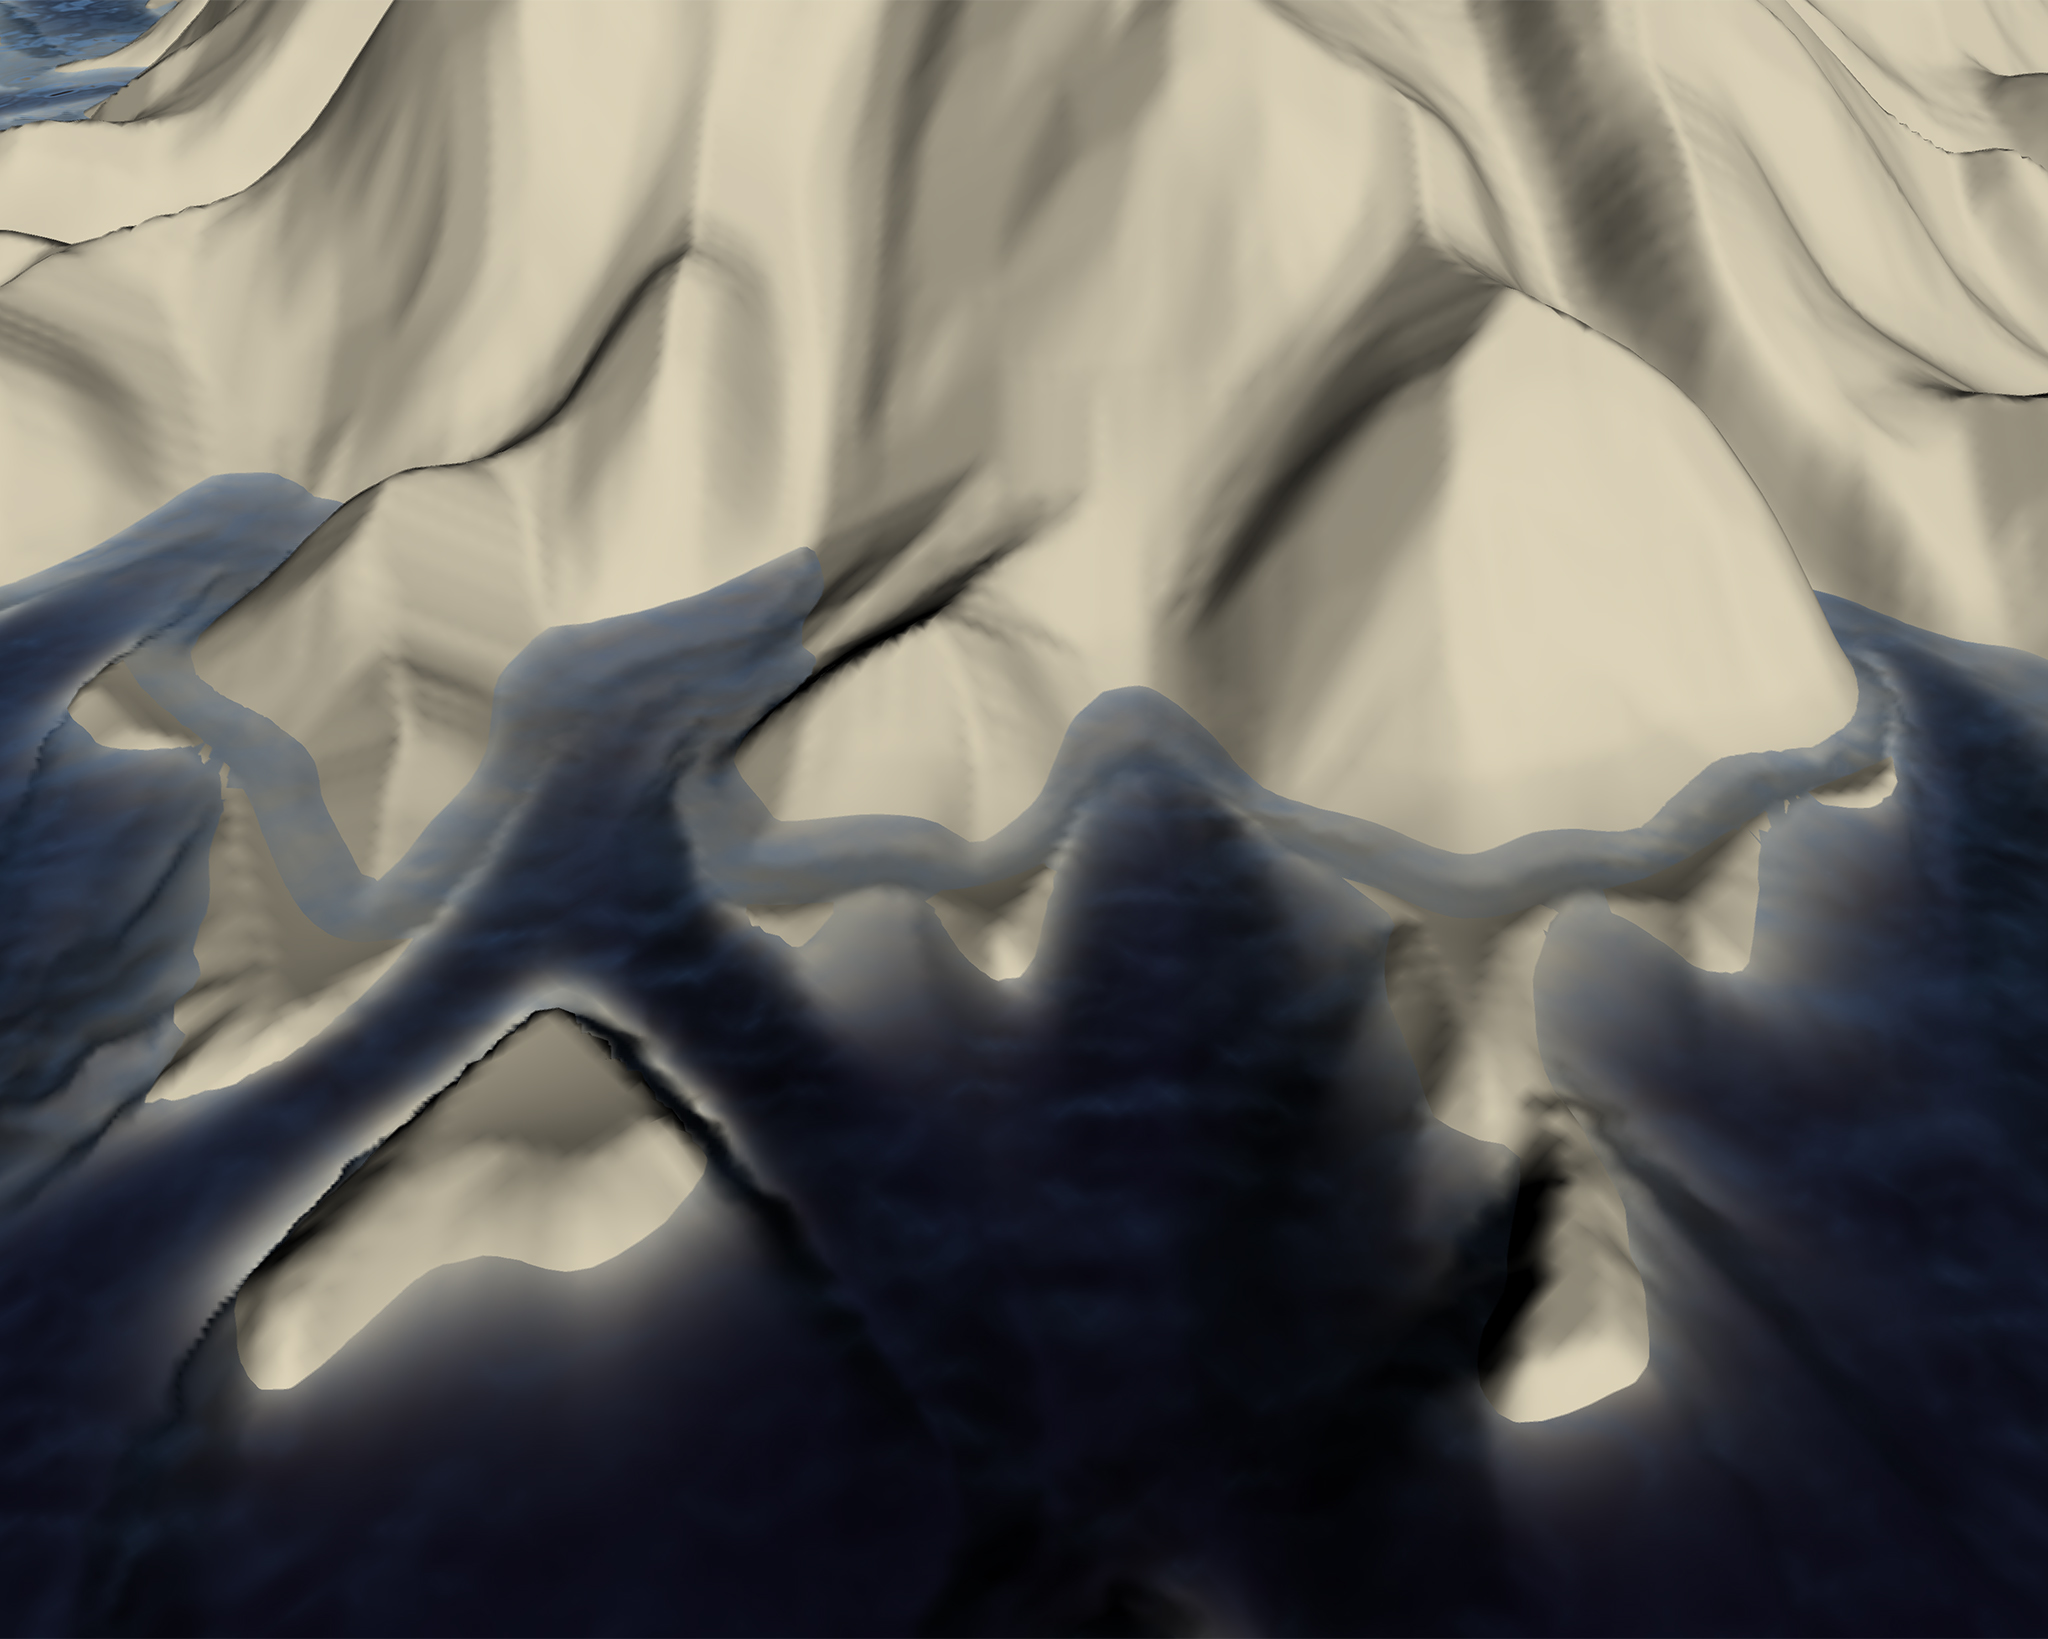
\includegraphics[width=0.7\textwidth]{example_coral_reef}
  \end{center}
  \caption{Virtualno obogatena skulptura~\cite{vodnjak}. Rezultate računalniško generirane animacije z video projektorjem projeciramo na kamnito skulpturo, da ustvarimo vtis, kot da bi po skulpturi polzele vodne kapljice~\cite{video,solina2020skulpture}.}
  \label{pic1}
\end{figure}

\subsection{Podnapisi k slikam in tabelam}

Vsaki sliki ali tabeli moramo dodati podnapis, ki nam pojasnjuje, kaj je na sliki ali tabeli, obrazloži vse morebitne okrajšave, pojasni glavna dognanja. Ne bojte se daljših opisov.
Če nekdo le prelista zaključno delo, naj bi že iz slik in njihovih podnapisov lahko na grobo razbral, kakšno temo naloga obravnava.

Če slike povzamemo iz drugih virov, se moramo v podnapisu k taki sliki nujno sklicujemo na ta vir!

\subsection{Vključevanje več slik in tabel hkrati}

Pri pisanju zaključnega dela se pogosto pojavi potreba po prikazovanju več slik ali tabel ene ob drugi. Za ta namen uporabljamo paket \ltx|subcaption|, ki predstavlja sodoben in podprt standard v \LaTeX u. 

V spletnih virih in starih predlogah študenti prepogosto najdejo in uporabijo paketa \ltx|subfigure| ali \ltx|subfig|. Oba paketa sta zastarela in pogosto povzročata težave pri prevajanju ali konflikte z drugimi paketi (npr. pri generiranju hiperpovezav). Teh dveh paketov zato \textbf{ne uporabljajte}. Prav tako se za razporejanje slik v mrežo ne poslužujte paketa \ltx|TikZ|. Ta paket je sicer izjemno močno orodje, a je namenjen risanju vektorskih shem in je za preprosto razporejanje slik odločno preveč kompleksen.

Za uporabo sodobnega pristopa v preambulo dokumenta dodajte ukaz:\\
\ltx|\usepackage{subcaption}|.
Paket nam ponuja dve okolji: \ltx|subfigure| za slike in \ltx|subtable| za tabele. Obe okolji v ozadju delujeta na podobnem principu kot standardno okolje \ltx|minipage| (ki ga v \LaTeX u pogosto uporabljamo za postavljanje povsem neodvisnih blokov vsebin enega ob drugega), saj obema podamo eksplicitno širino, ki jo bosta zavzela.

Ker so slike in tabele plavajoči objekti, ne smemo nikoli predpostavljati, kje natančno na strani se bodo izrisale. Na vse elemente se v besedilu vedno sklicujemo izključno z ukazom \ltx|\ref|, pred katerim uporabimo nedeljivi presledek (\ltx|~|).

\subsubsection{Več slik s podnaslovi}

Kadar želimo vsaki sliki dodeliti svojo oznako (npr. a, b) in podnaslov, uporabimo okolje \ltx|subfigure|. Širino posamezne podslike določimo z ulomkom širine besedila, npr. \ltx|0.48\textwidth|. Vmesni prostor do polne širine zapolnimo z ukazom \ltx|\hfill|. Na sliki~\ref{sl:dve_sliki} lahko vidimo primer dveh slik, ki sta postavljeni ena ob drugi.

\begin{figure}[htbp]
    \centering
    \begin{subfigure}[b]{0.48\textwidth}
        \centering
        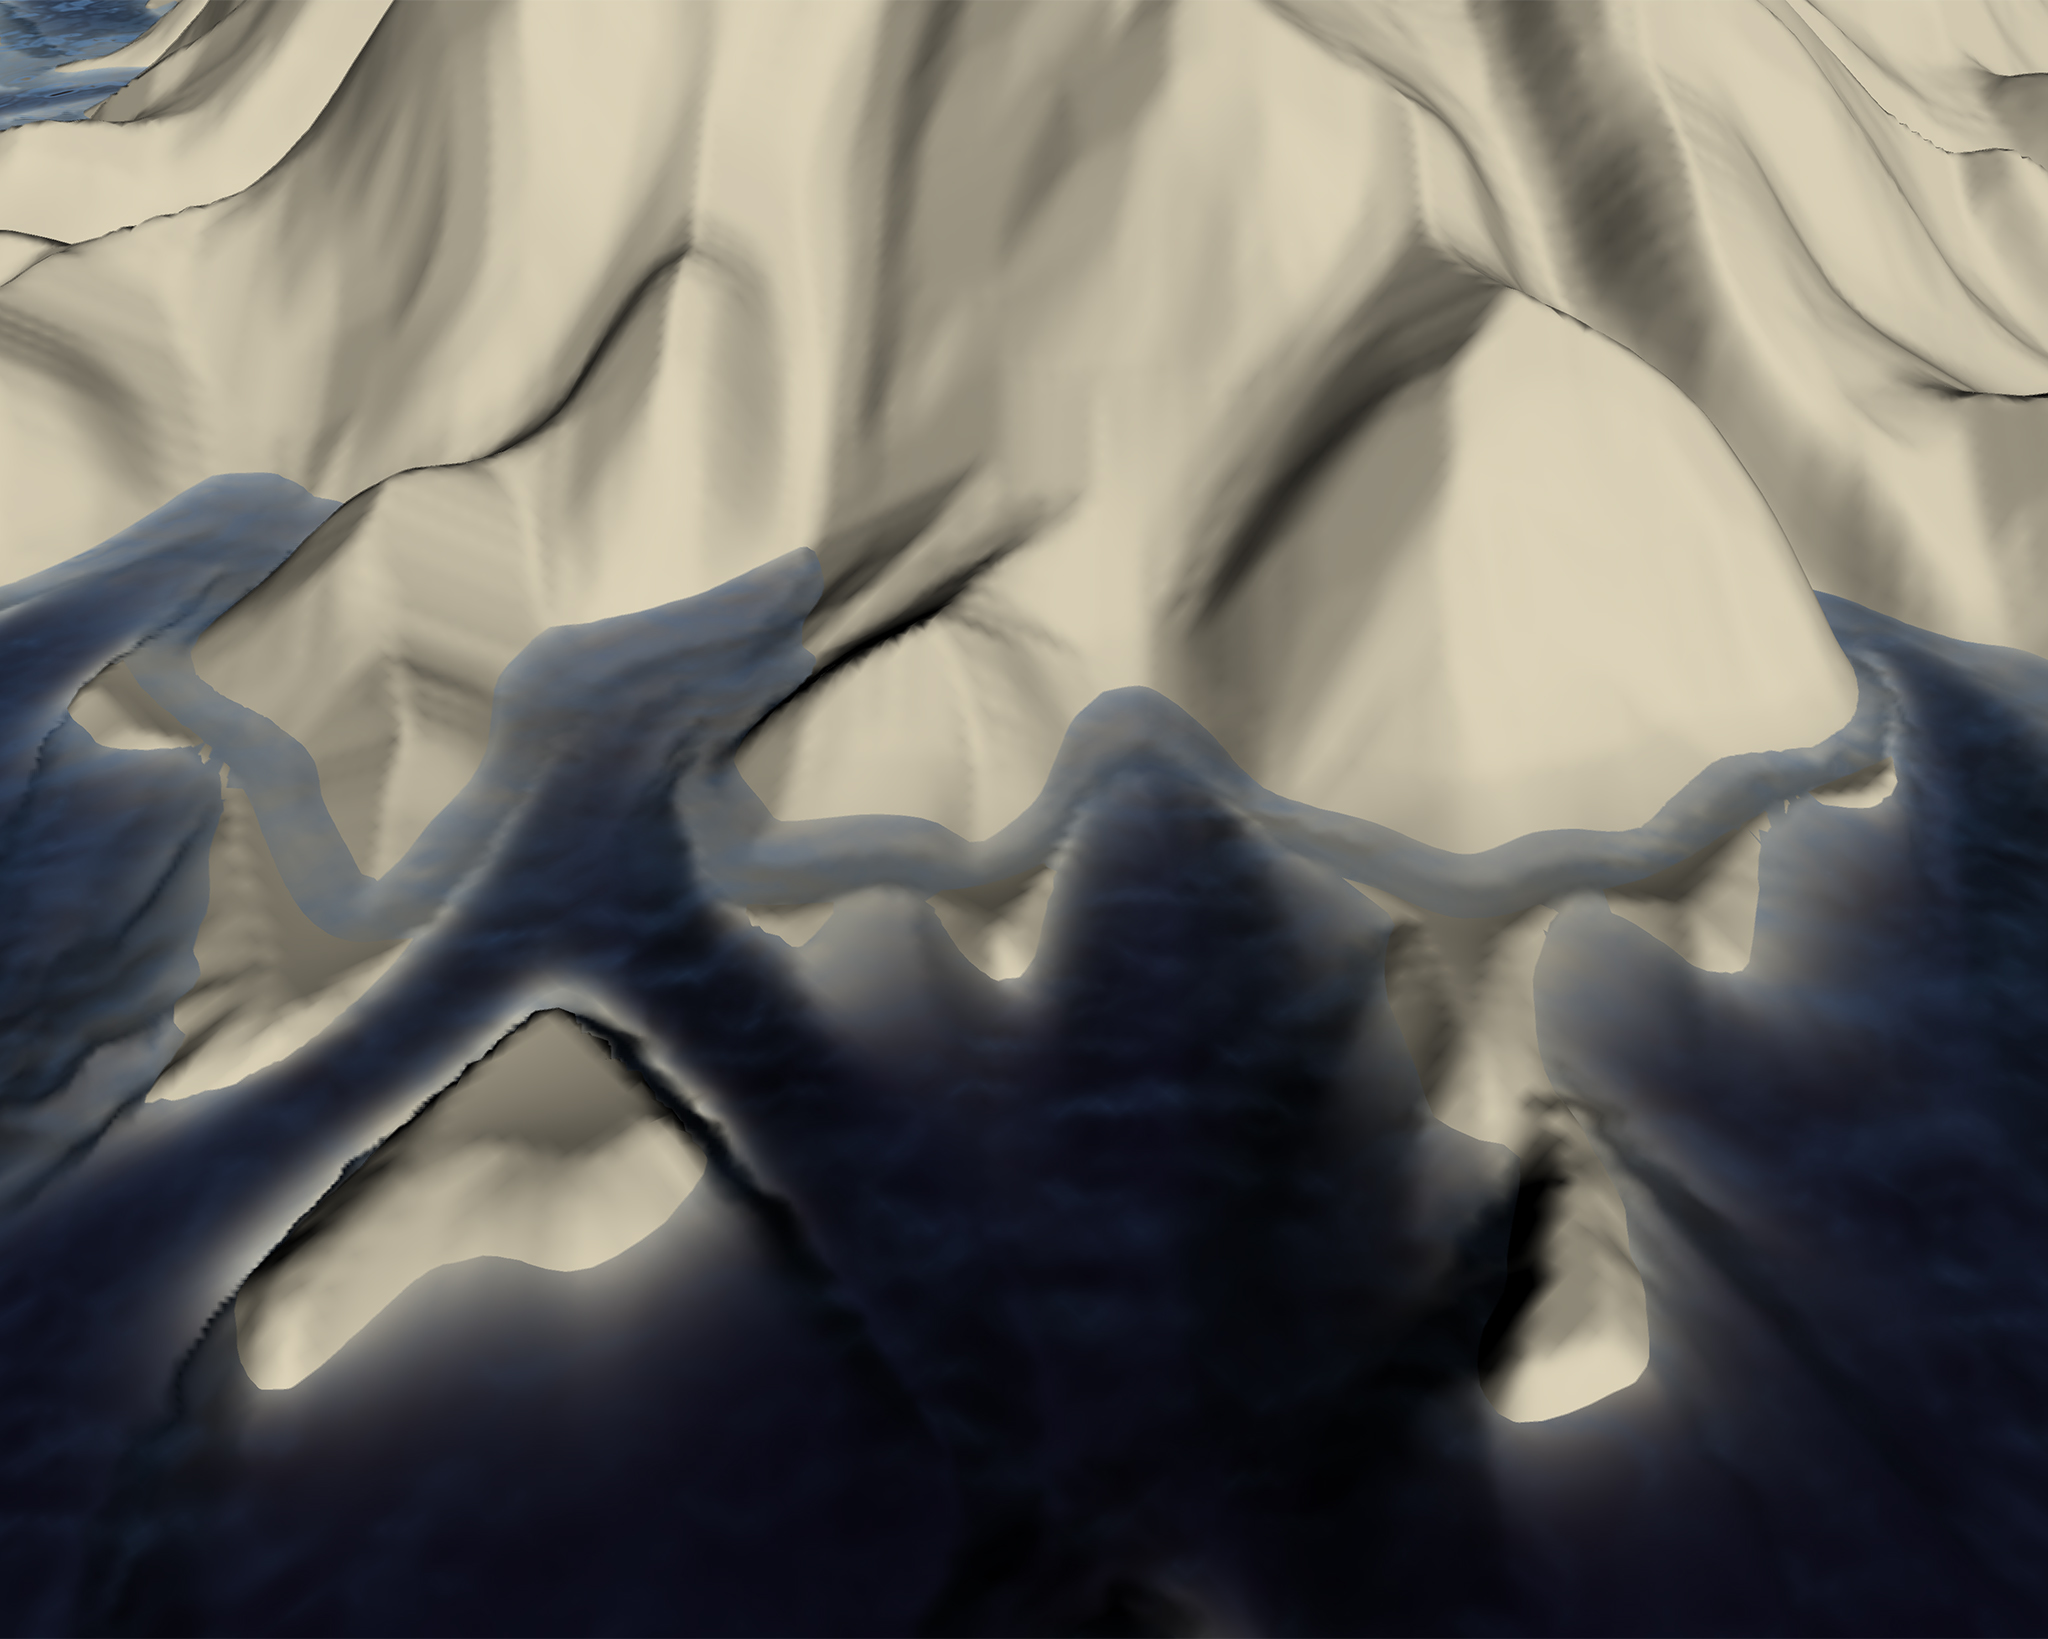
\includegraphics[width=\textwidth]{example_coral_reef}
        \caption{Podnaslov leve slike.}
        \label{sl:leva}
    \end{subfigure}
    \hfill
    \begin{subfigure}[b]{0.48\textwidth}
        \centering
        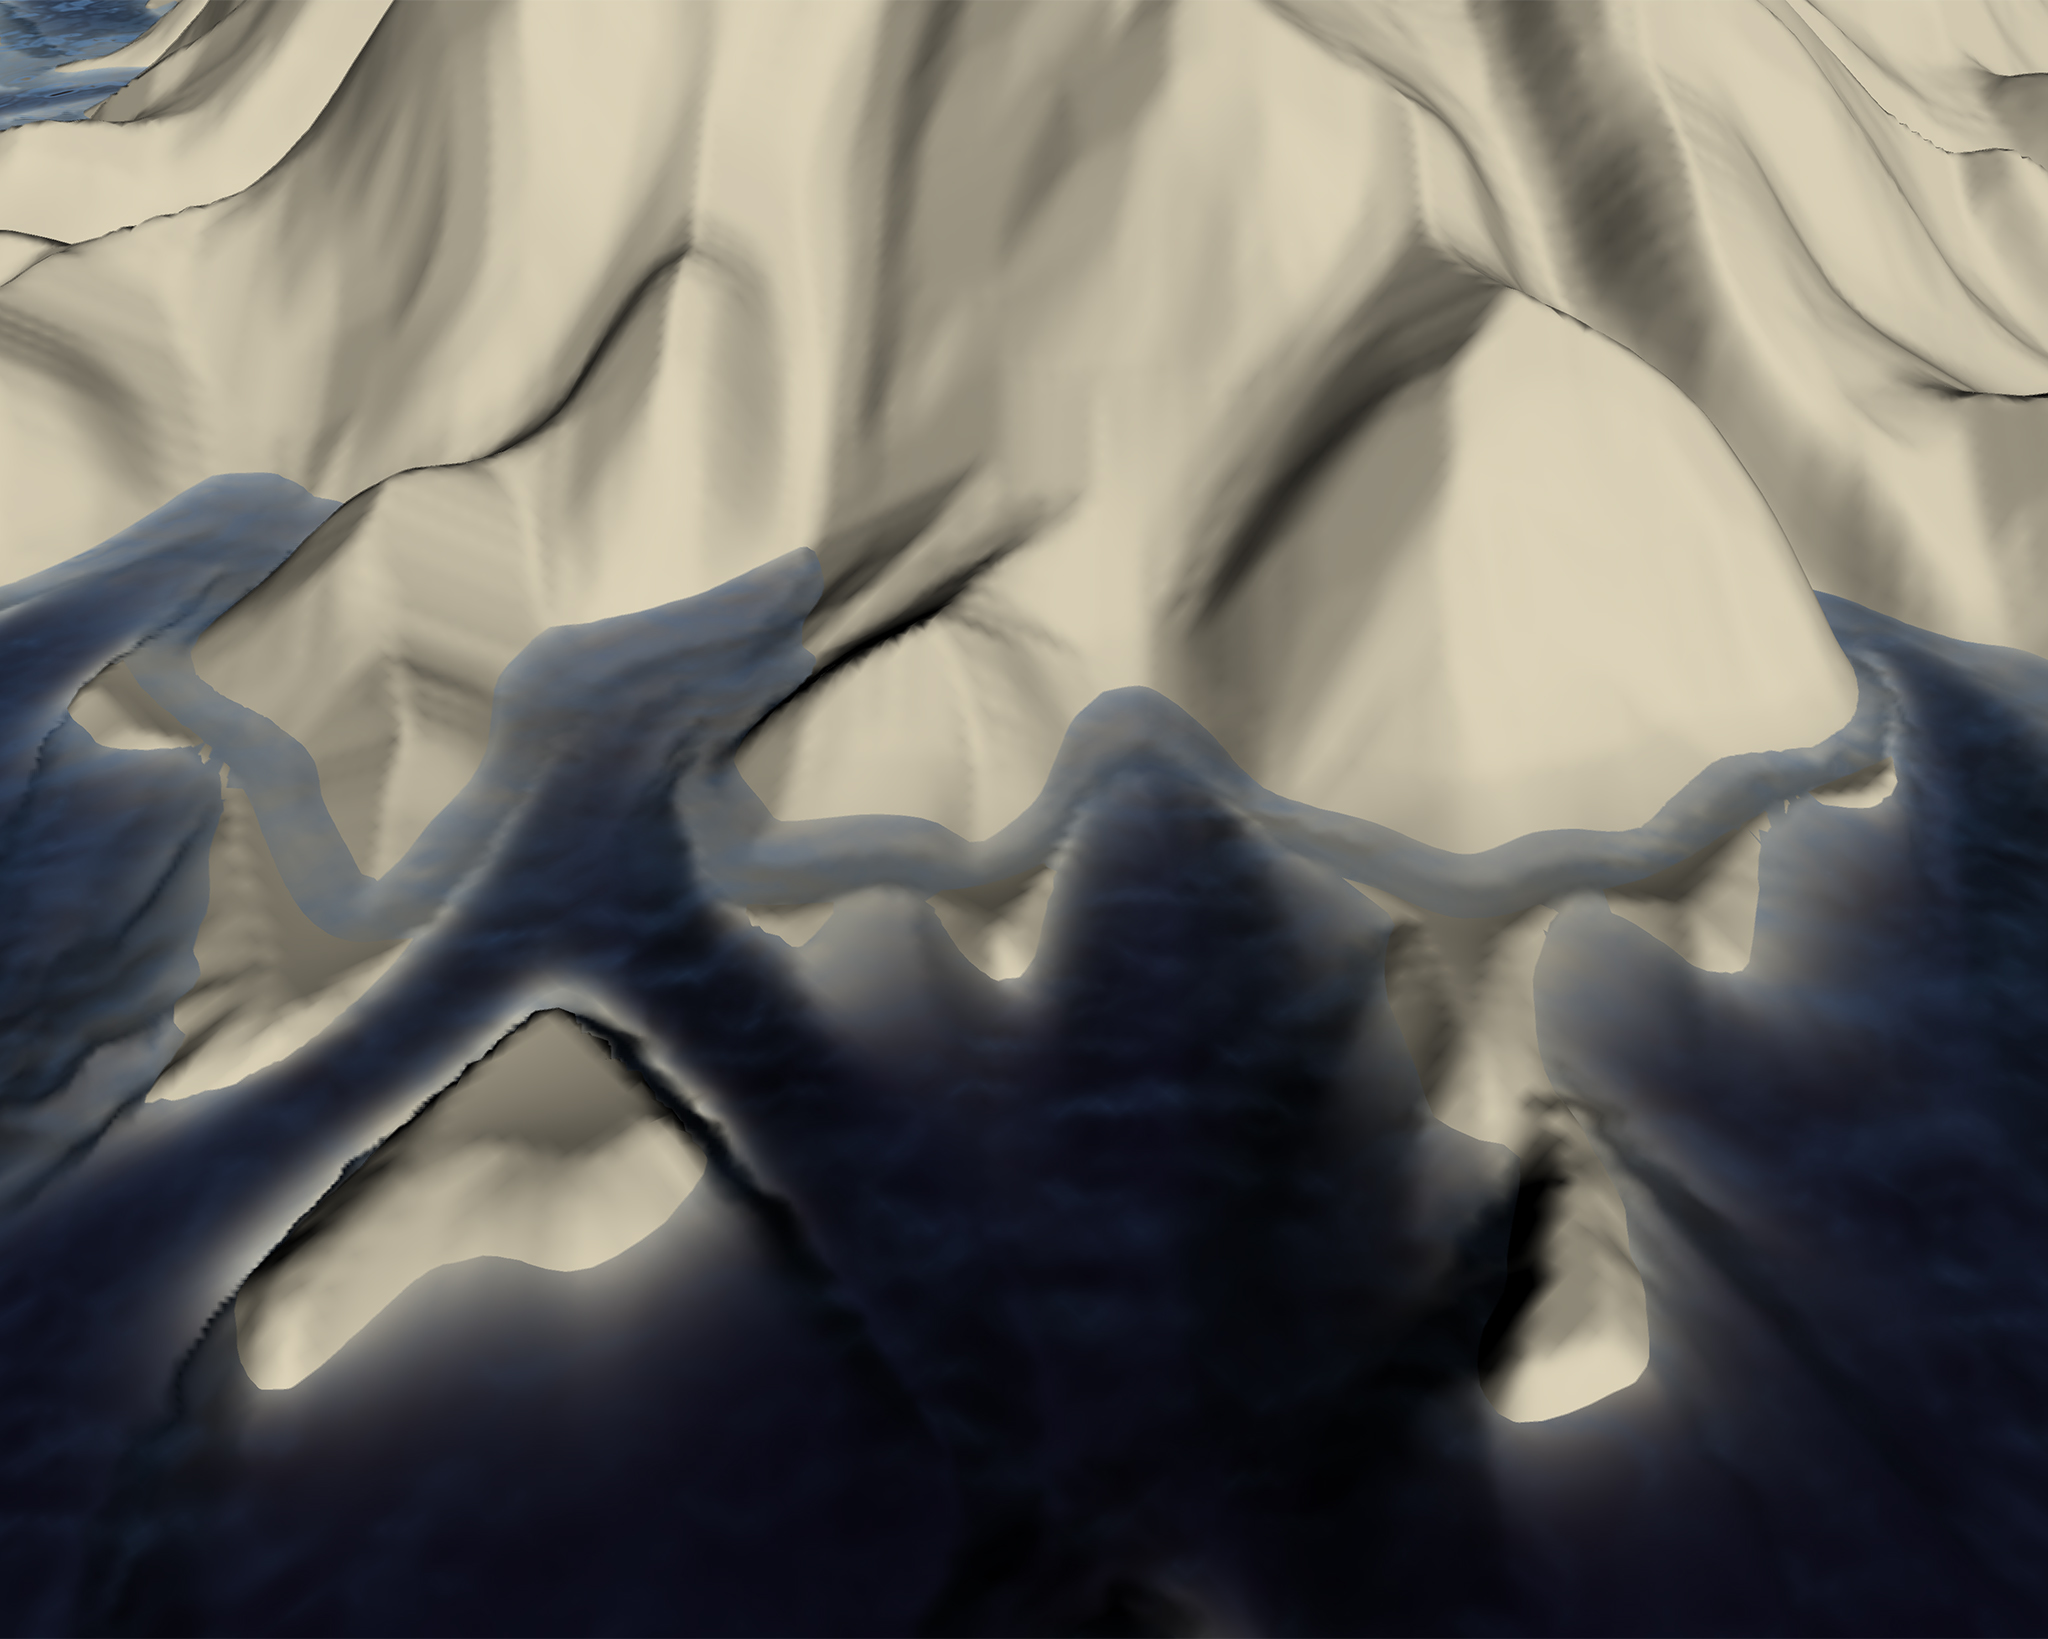
\includegraphics[width=\textwidth]{example_coral_reef}
        \caption{Podnaslov desne slike.}
        \label{sl:desna}
    \end{subfigure}
    \caption{Skupni naslov, ki opisuje obe sliki.}
    \label{sl:dve_sliki}
\end{figure}

Za prehod v novo vrsto znotraj istega plavajočega objekta preprosto izpustimo prazno vrstico in po želji dodamo nekaj vertikalnega prostora z ukazom \ltx|\vspace|. Na tak način je zgrajena mreža štirih slik na sliki~\ref{sl:mreza_2x2}.

\begin{figure}[htbp]
    \centering
    \begin{subfigure}[b]{0.48\textwidth}
        \centering
        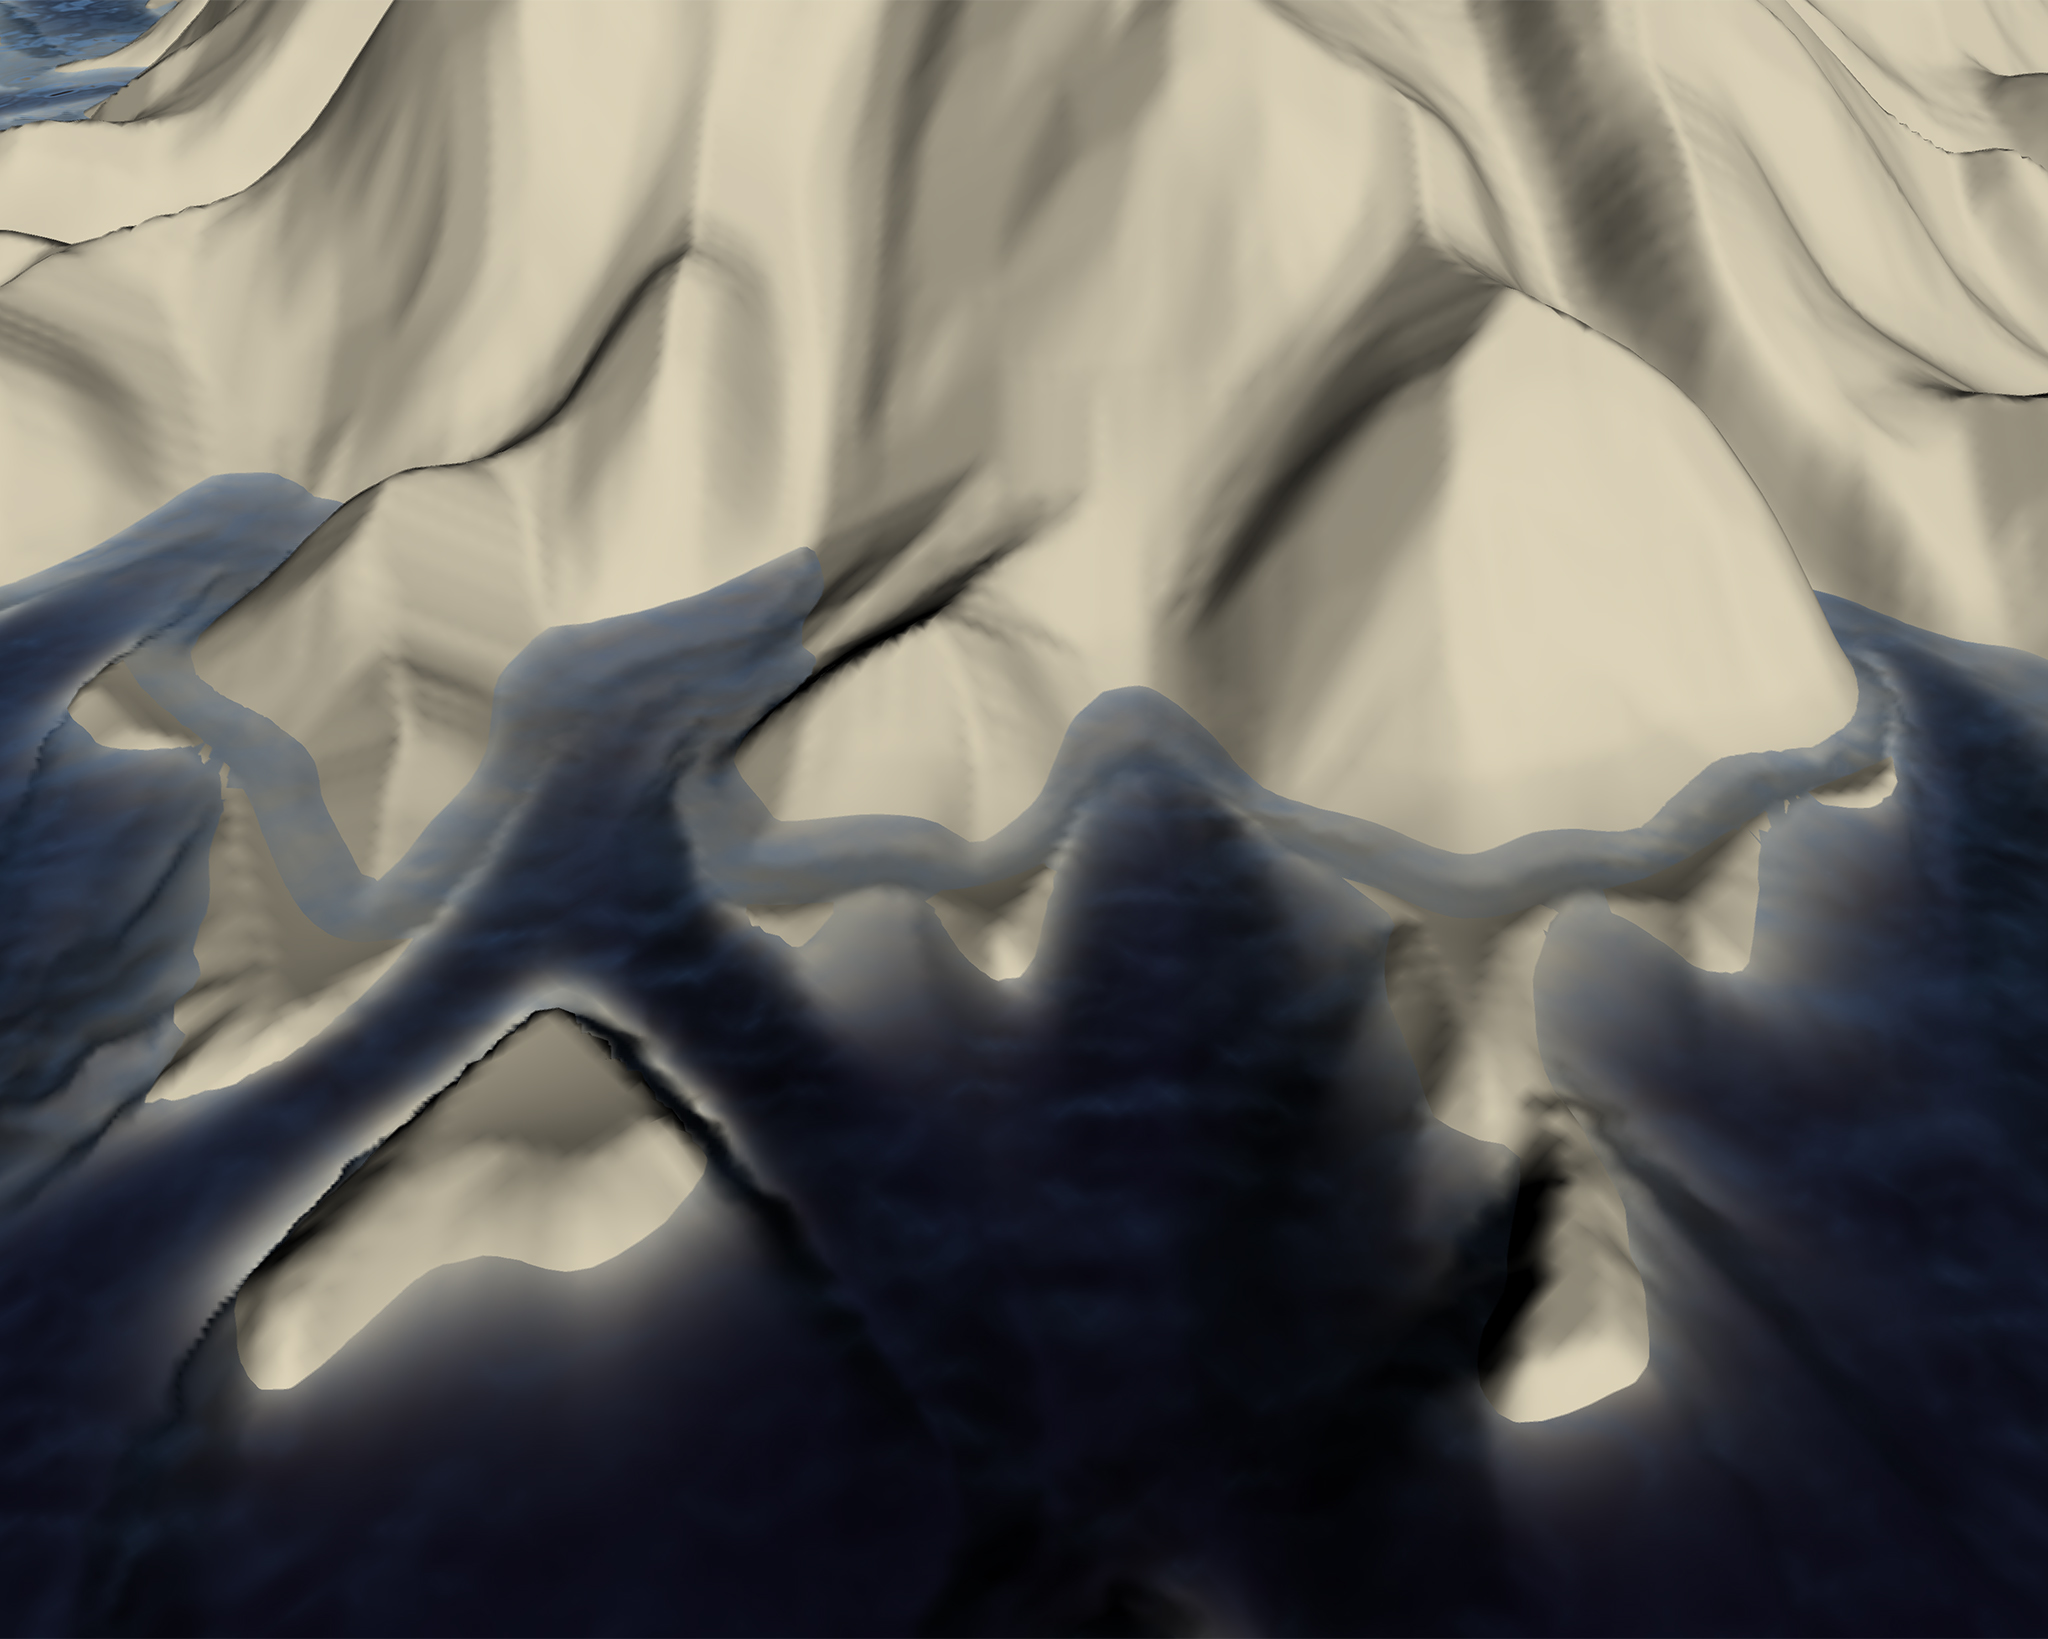
\includegraphics[width=\textwidth]{example_coral_reef}
        \caption{Zgoraj levo.}
    \end{subfigure}
    \hfill
    \begin{subfigure}[b]{0.48\textwidth}
        \centering
        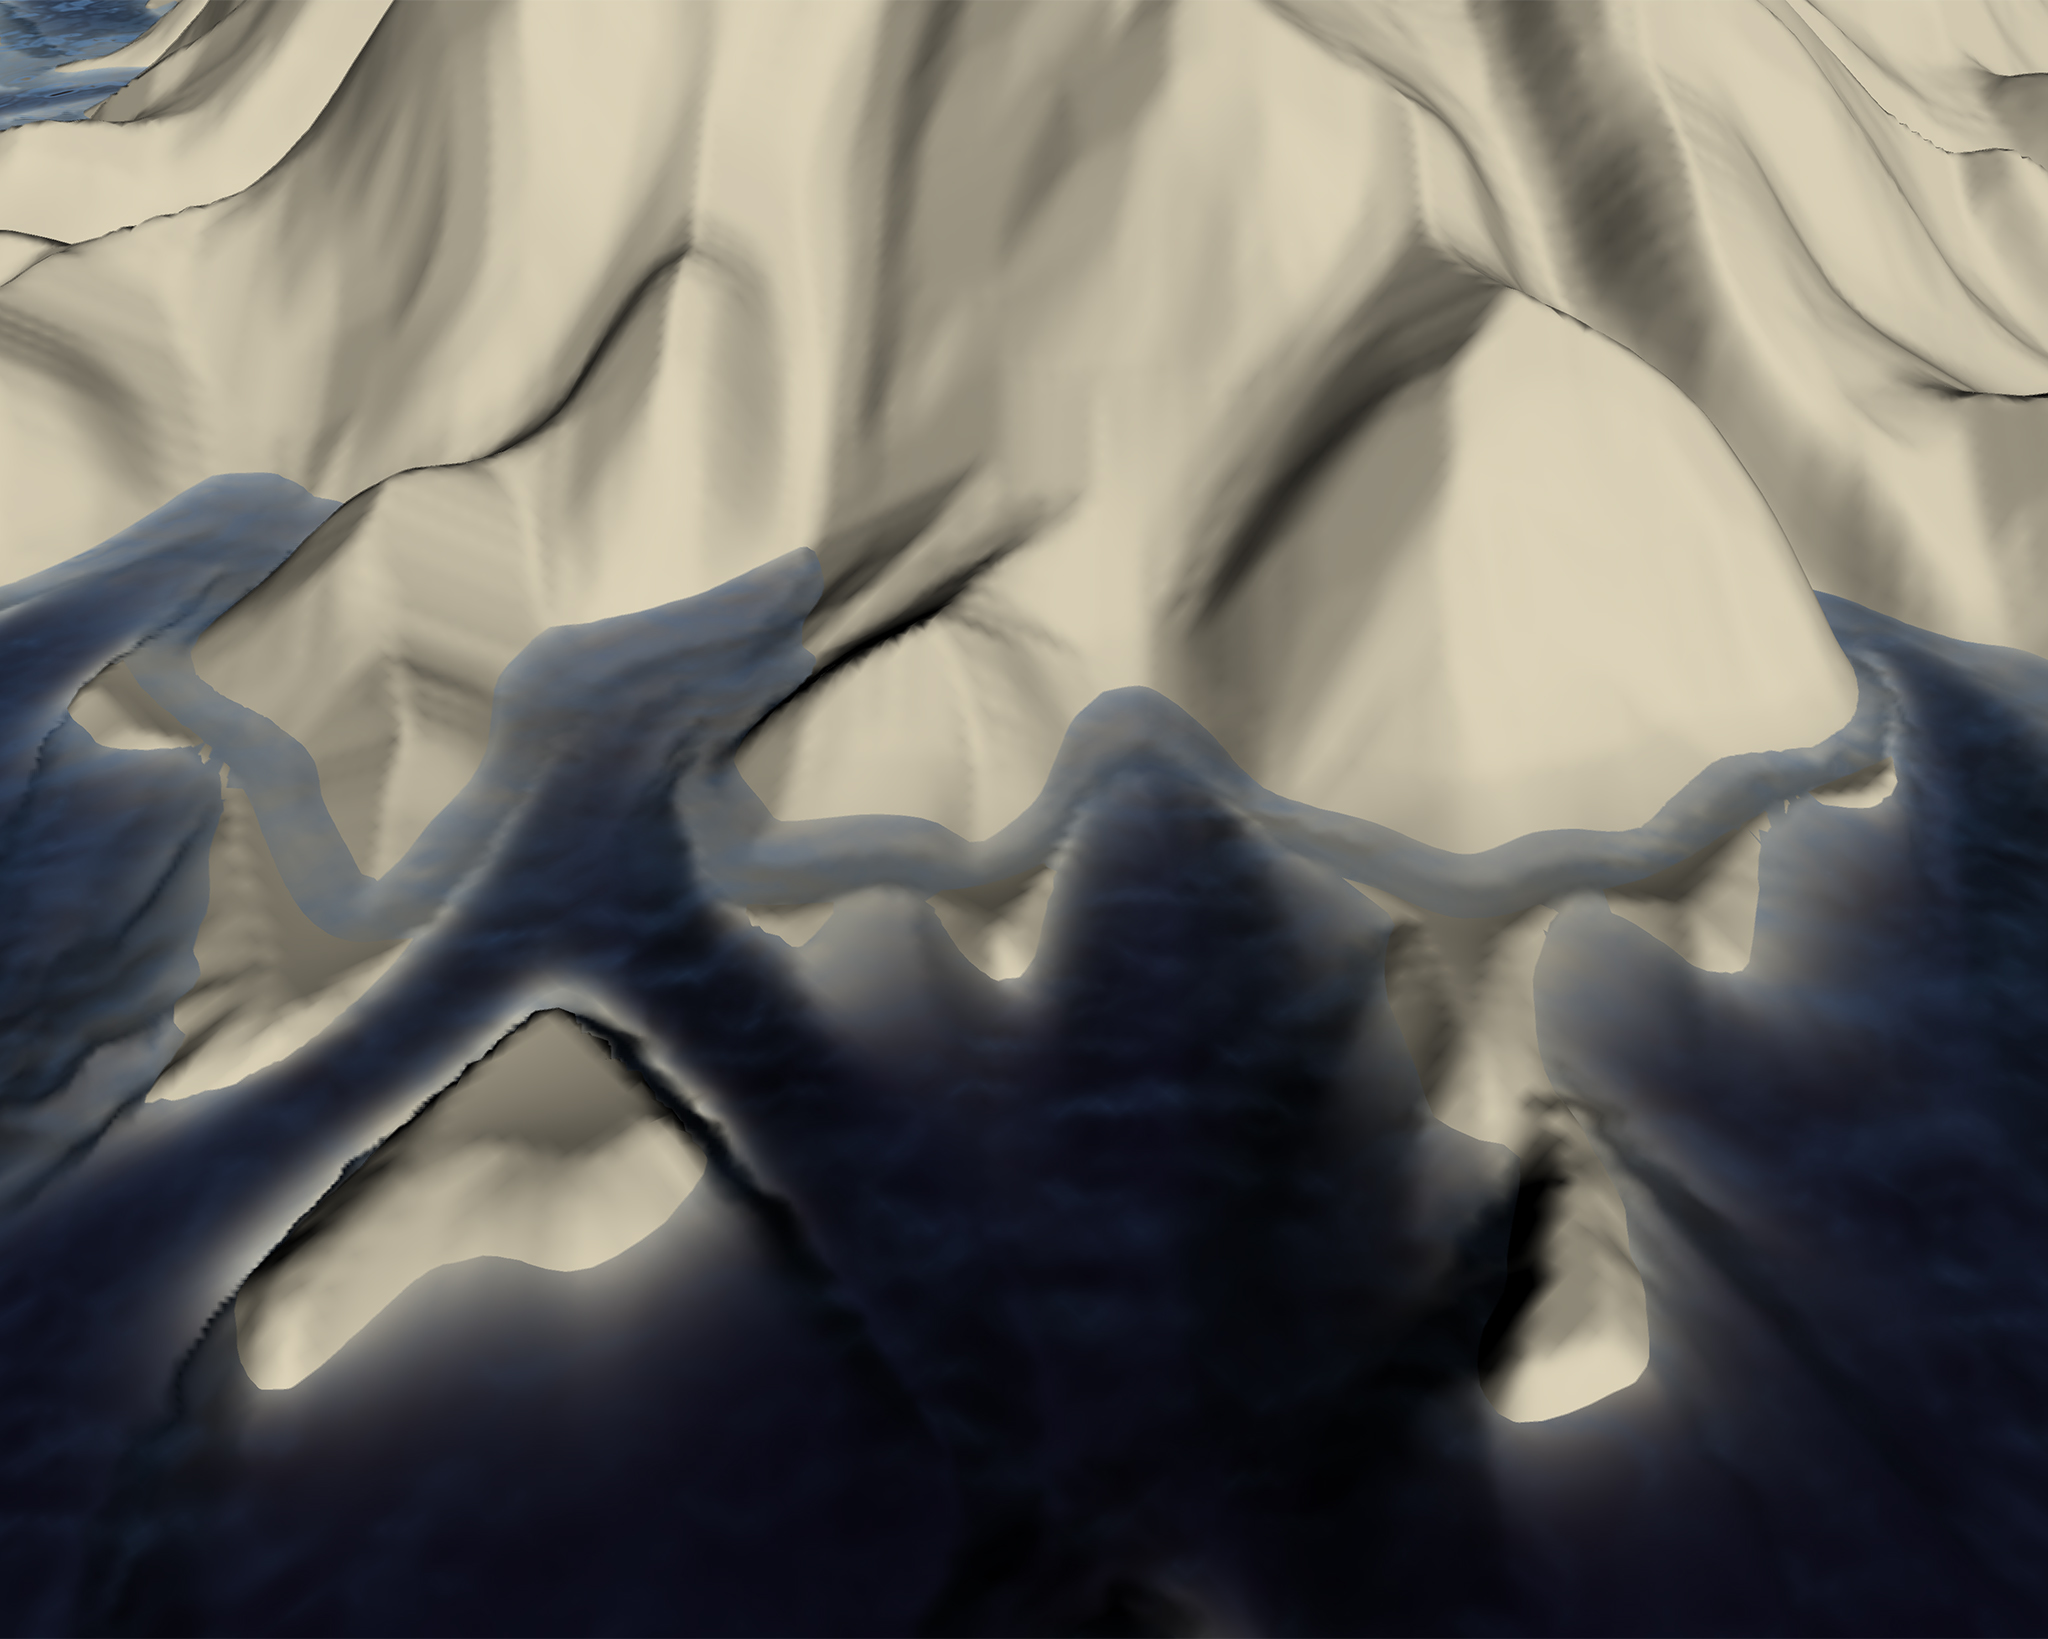
\includegraphics[width=\textwidth]{example_coral_reef}
        \caption{Zgoraj desno.}
    \end{subfigure}
    
    \vspace{0.5cm} % Vertikalni razmik med vrsticama
    
    \begin{subfigure}[b]{0.48\textwidth}
        \centering
        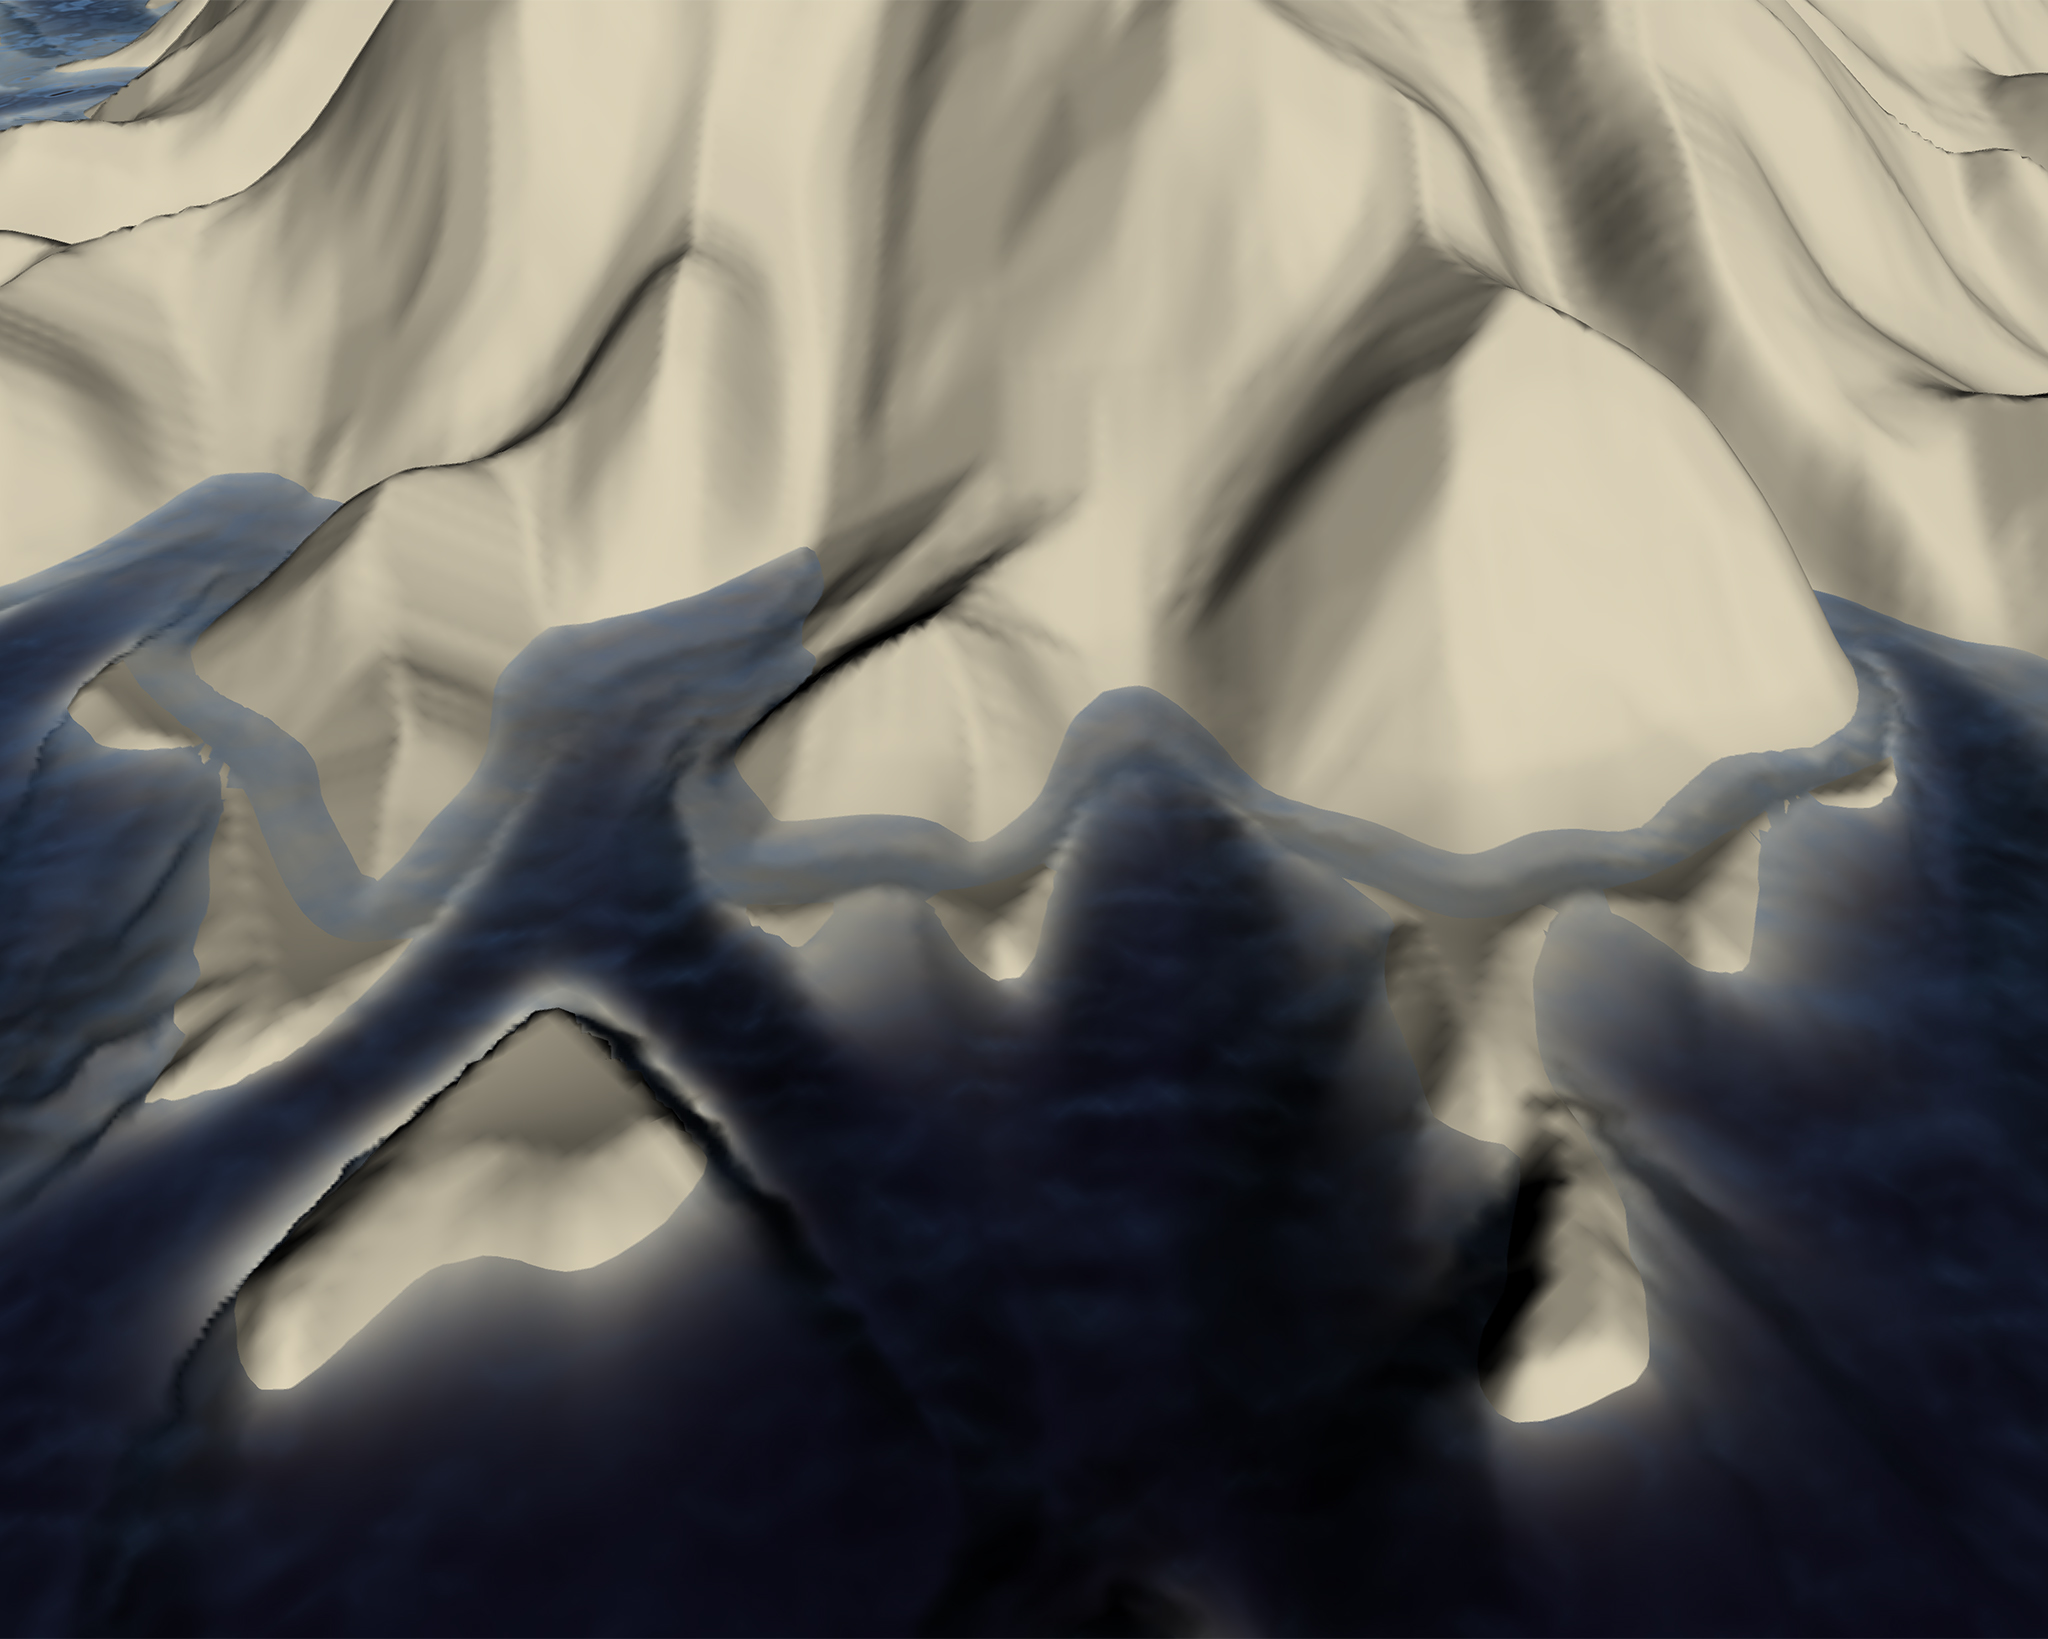
\includegraphics[width=\textwidth]{example_coral_reef}
        \caption{Spodaj levo.}
    \end{subfigure}
    \hfill
    \begin{subfigure}[b]{0.48\textwidth}
        \centering
        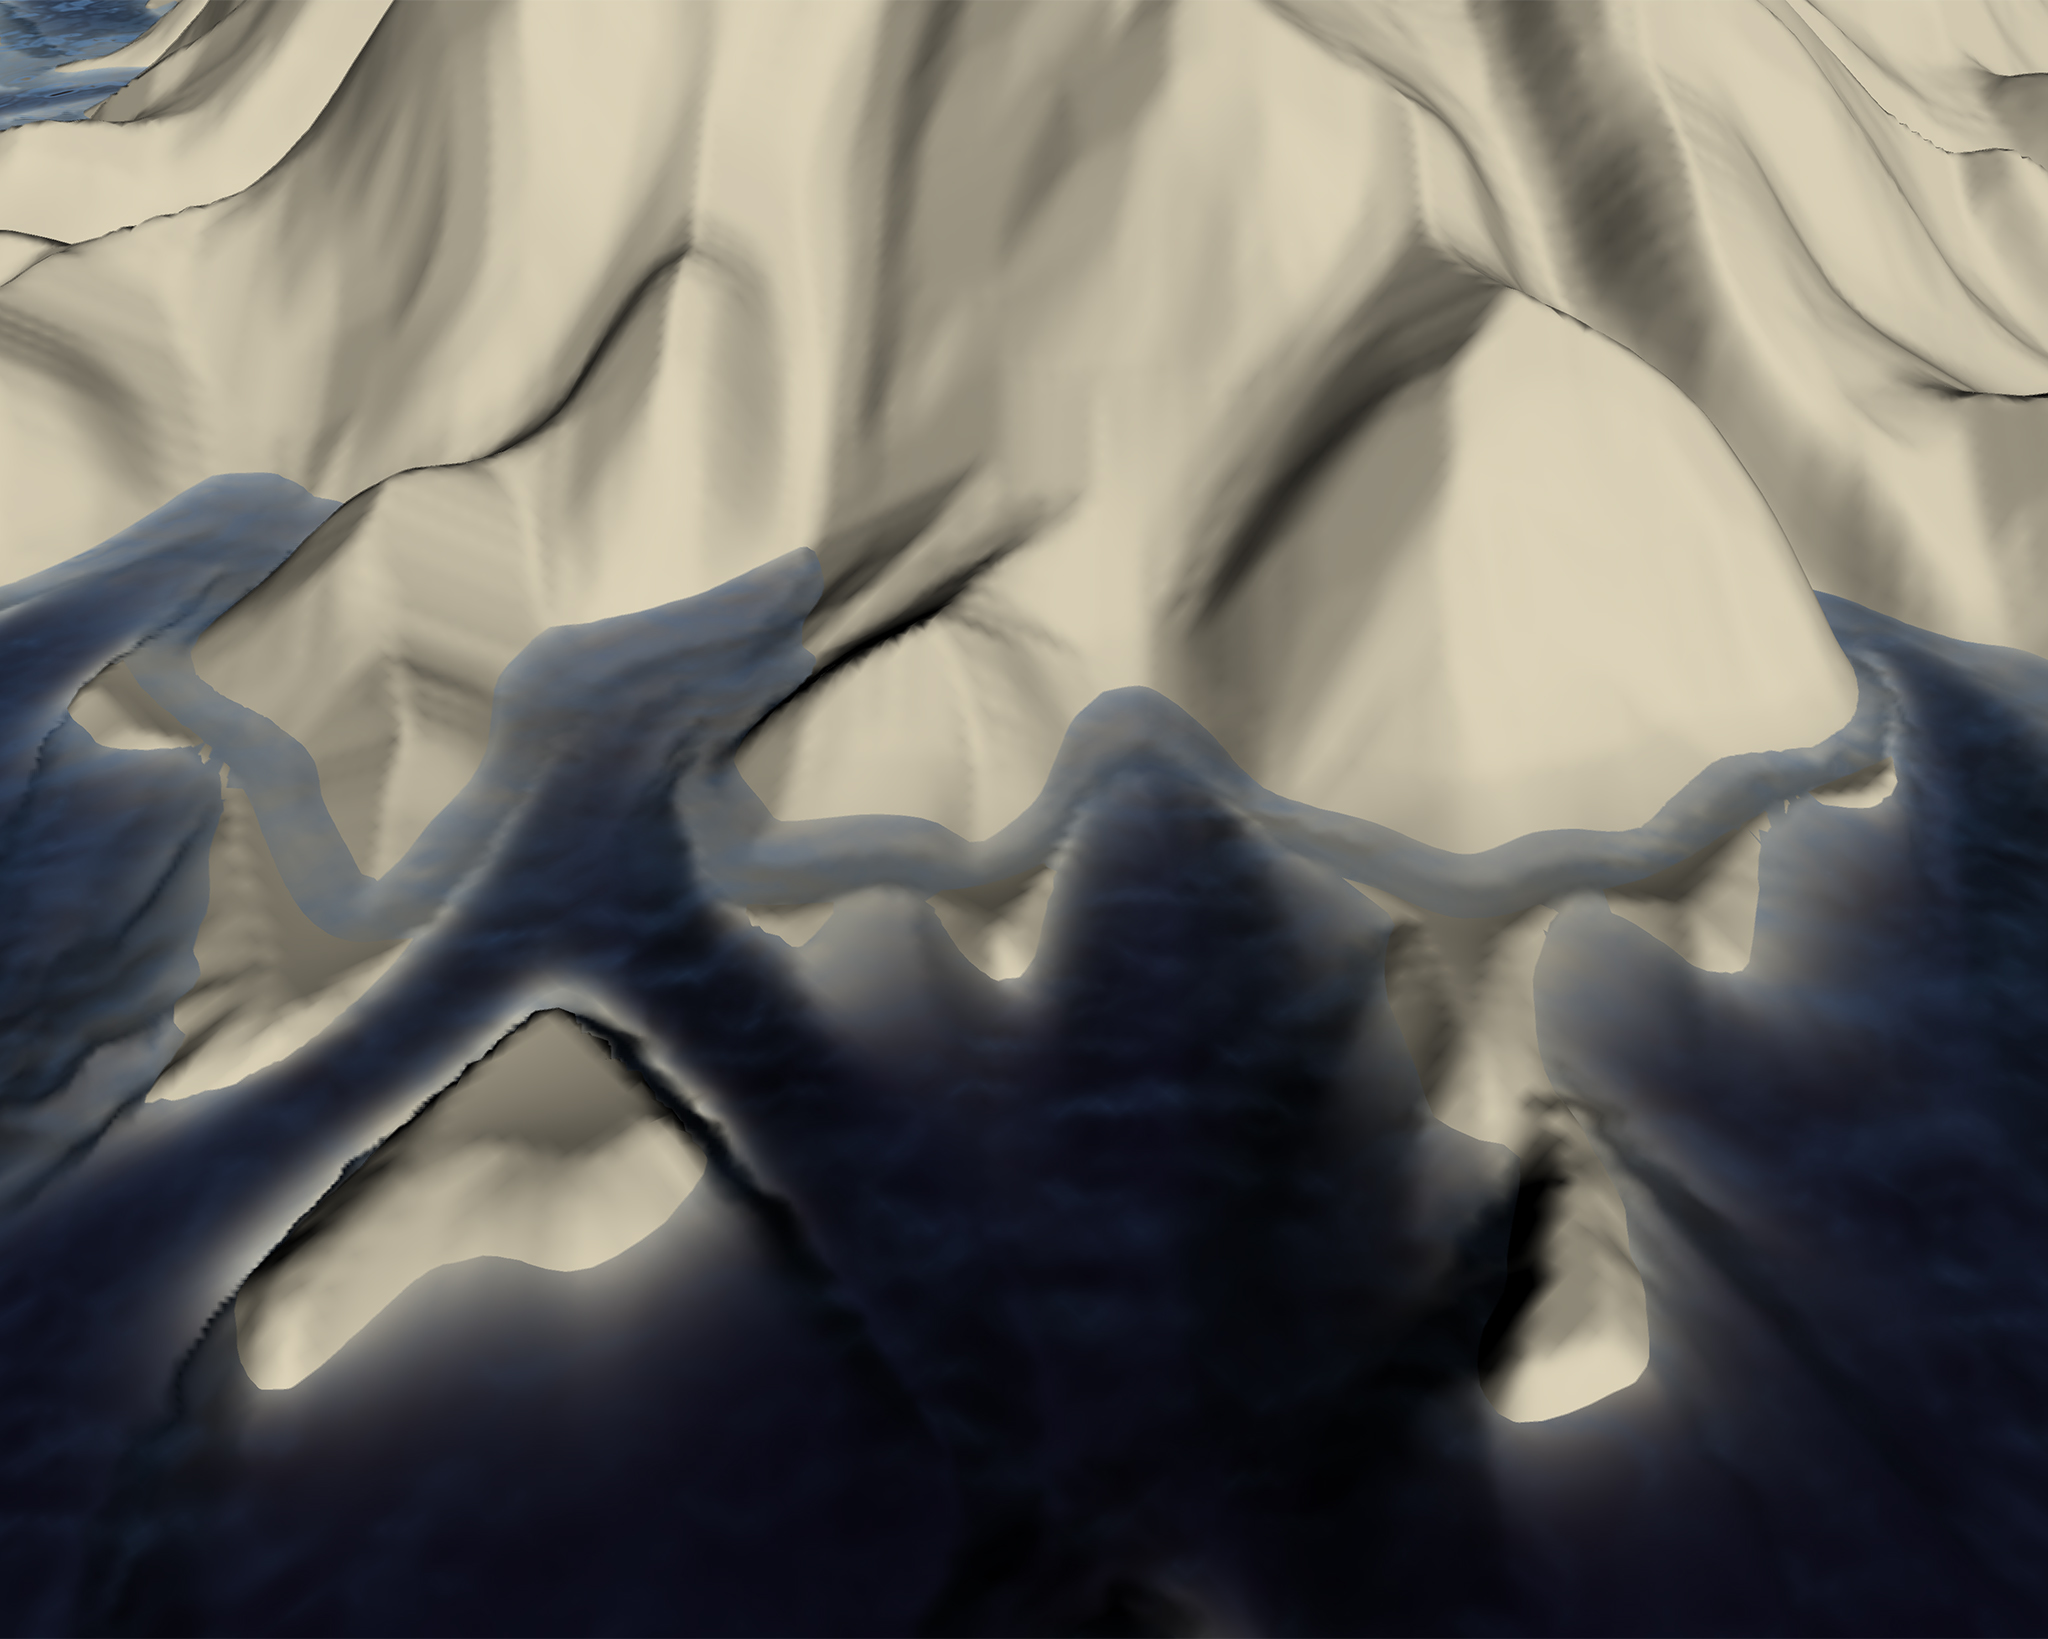
\includegraphics[width=\textwidth]{example_coral_reef}
        \caption{Spodaj desno.}
    \end{subfigure}
    \caption{Mreža štirih slik s posameznimi podnaslovi.}
    \label{sl:mreza_2x2}
\end{figure}

\subsubsection{Več slik brez podnaslovov (mreža brez presledkov)}

Če individualni podnaslovi niso potrebni in želimo le en skupen naslov celotne mreže slik, okolja \ltx|subfigure| sploh ne potrebujemo. Slike preprosto naložimo znotraj navadnega \ltx|figure| okolja in določimo njihovo velikost. 

Če želimo ustvariti neprekinjeno mrežo povsem \textbf{brez vmesnih presledkov} (kot to prikazuje slika~\ref{sl:mreza_4x2_brez_presledkov}), moramo poskrbeti za dve stvari:
\begin{enumerate}
    \item \textbf{Horizontalni presledki:} Širino določimo tako, da je vsota vseh širin v vrstici točno enaka \ltx|1.0\textwidth| (npr. štiri slike s širino \ltx|0.25\textwidth|). Na konec vsake vrstice z ukazom \ltx|\includegraphics| moramo dodati znak za komentar (\ltx|%|), s čimer preprečimo, da bi \LaTeX\ prelom vrstice interpretiral kot presledek.
    \item \textbf{Vertikalni presledki:} Znotraj posebnega bloka moramo uporabiti ukaz\\
    \ltx|\offinterlineskip|, ki v celoti izklopi samodejno vrivanje vertikalnega prostora med vrsticami. Pomembno je, da blok po zadnji sliki zapremo z \}, preden definiramo \ltx|\caption|.
\end{enumerate}

Pri sliki~\ref{sl:mreza_4x2_brez_presledkov} je vključena je tudi širša postavitev z uporabo bloka \ltx|{largefigure}|, namesto \ltx|{figure}|.

\begin{largefigure}[htbp]
    \centering
    {
    \offinterlineskip % Popolnoma izklopi vertikalni razmik med vrsticami znotraj tega bloka
    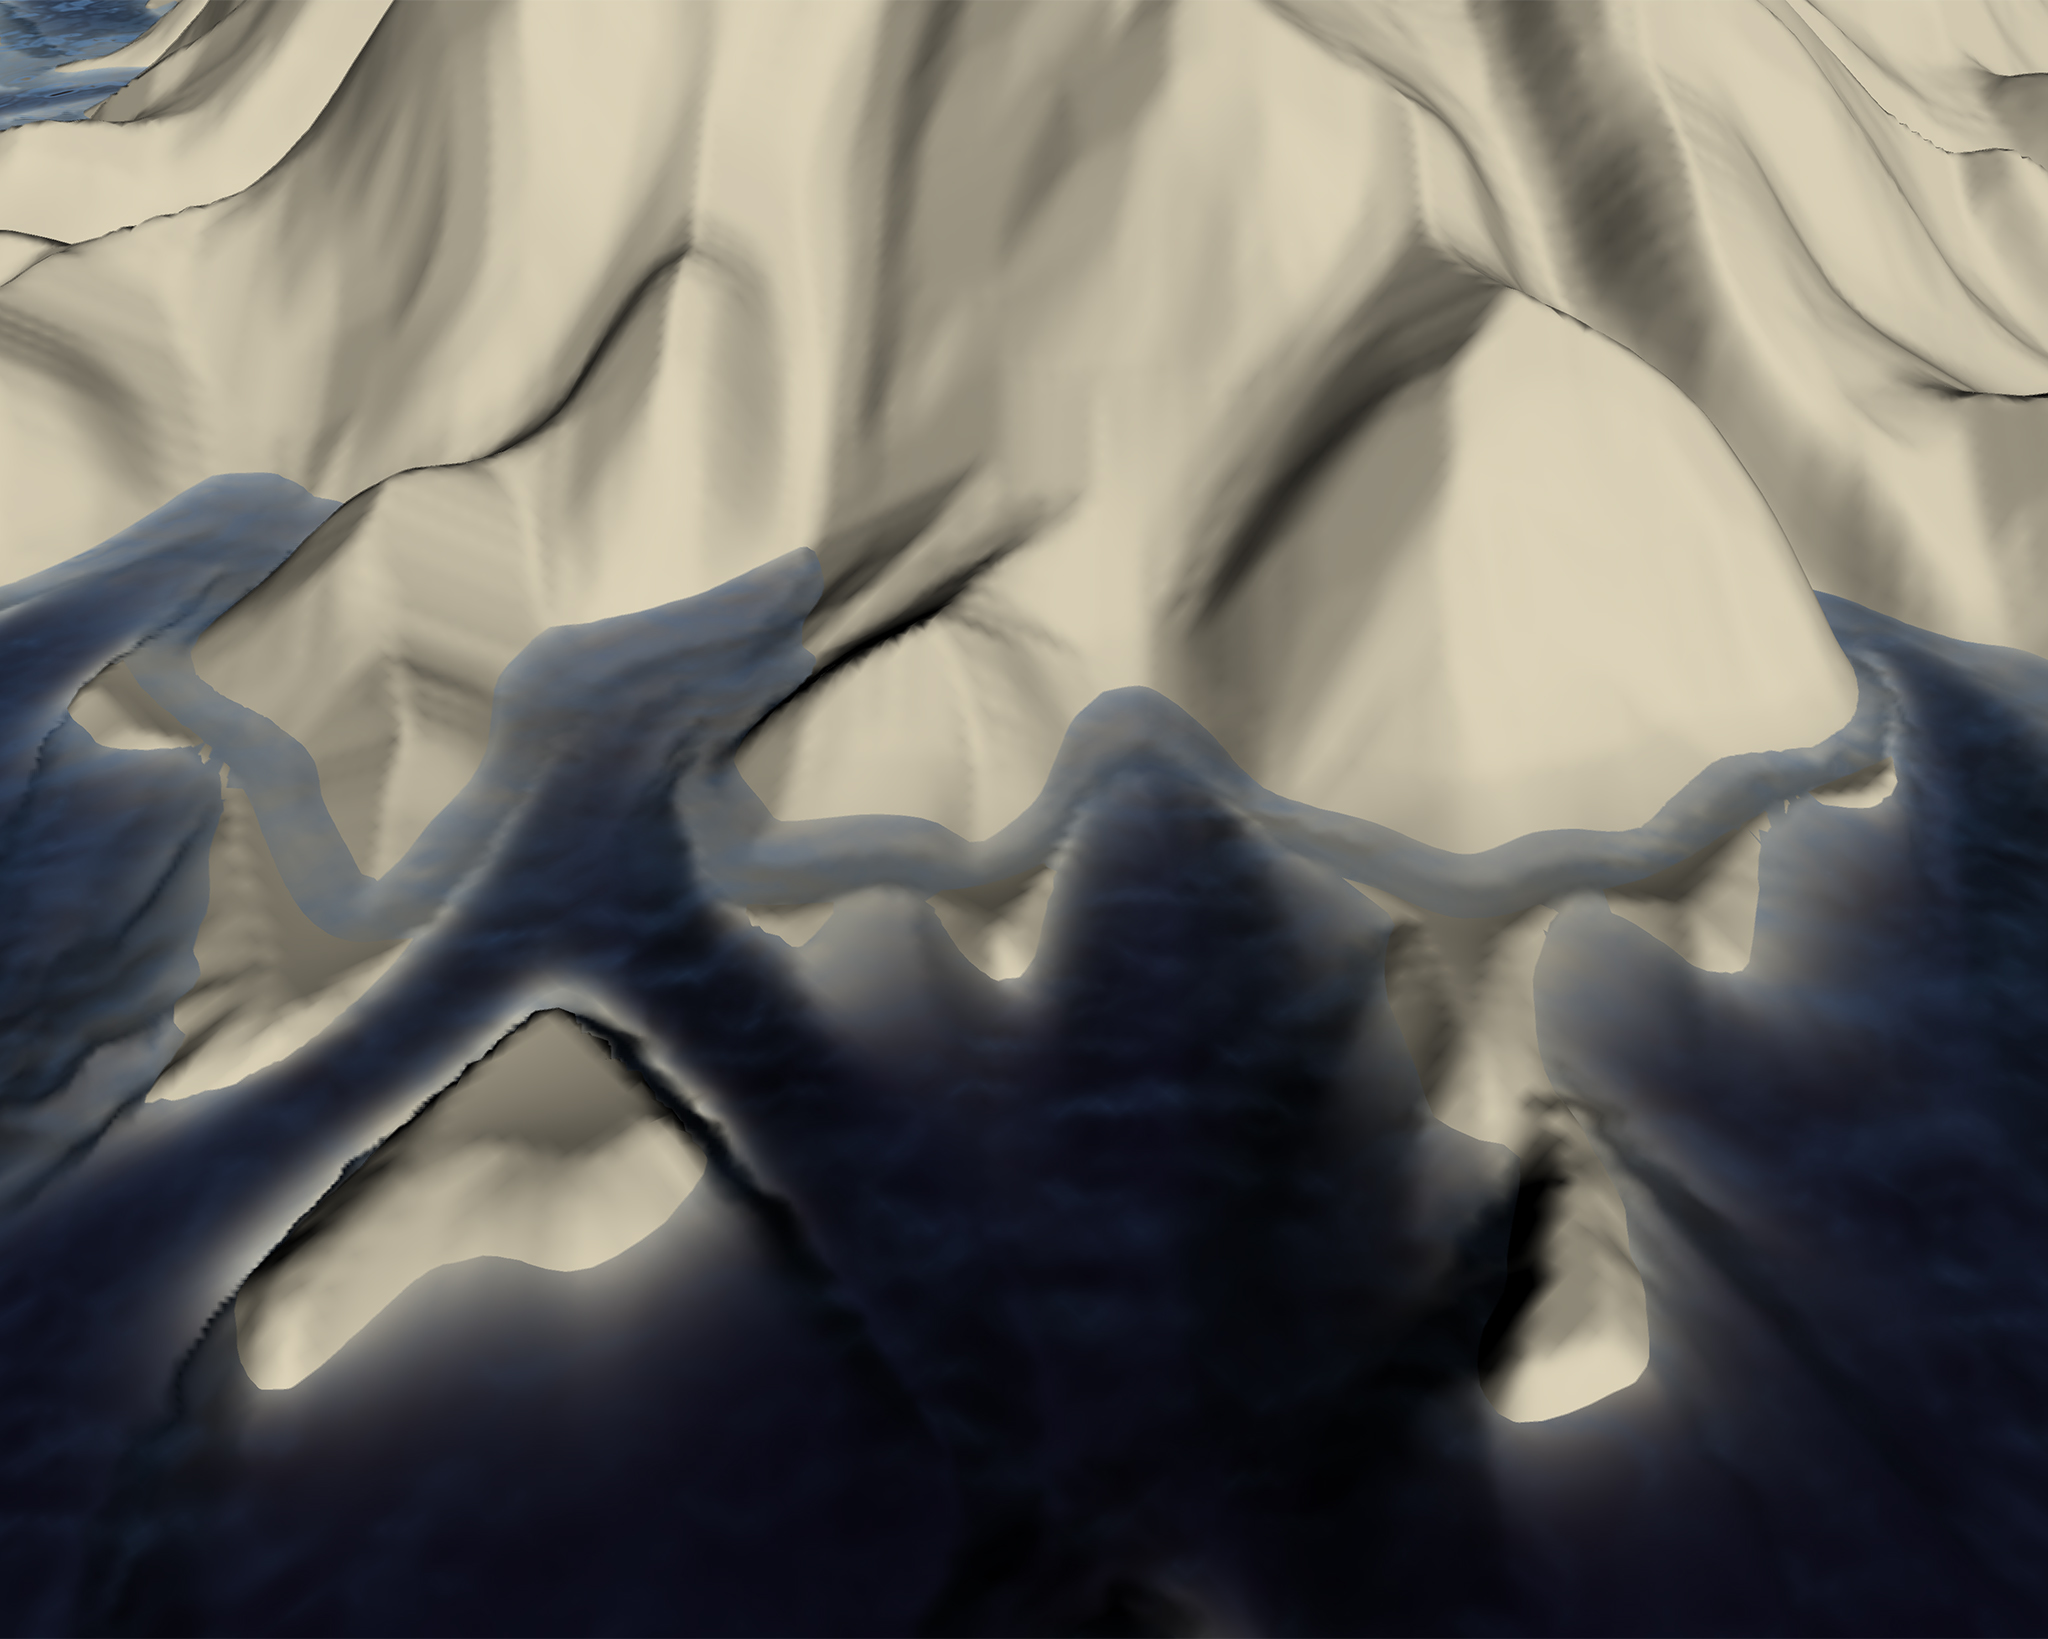
\includegraphics[width=0.25\linewidth]{example_coral_reef}%
    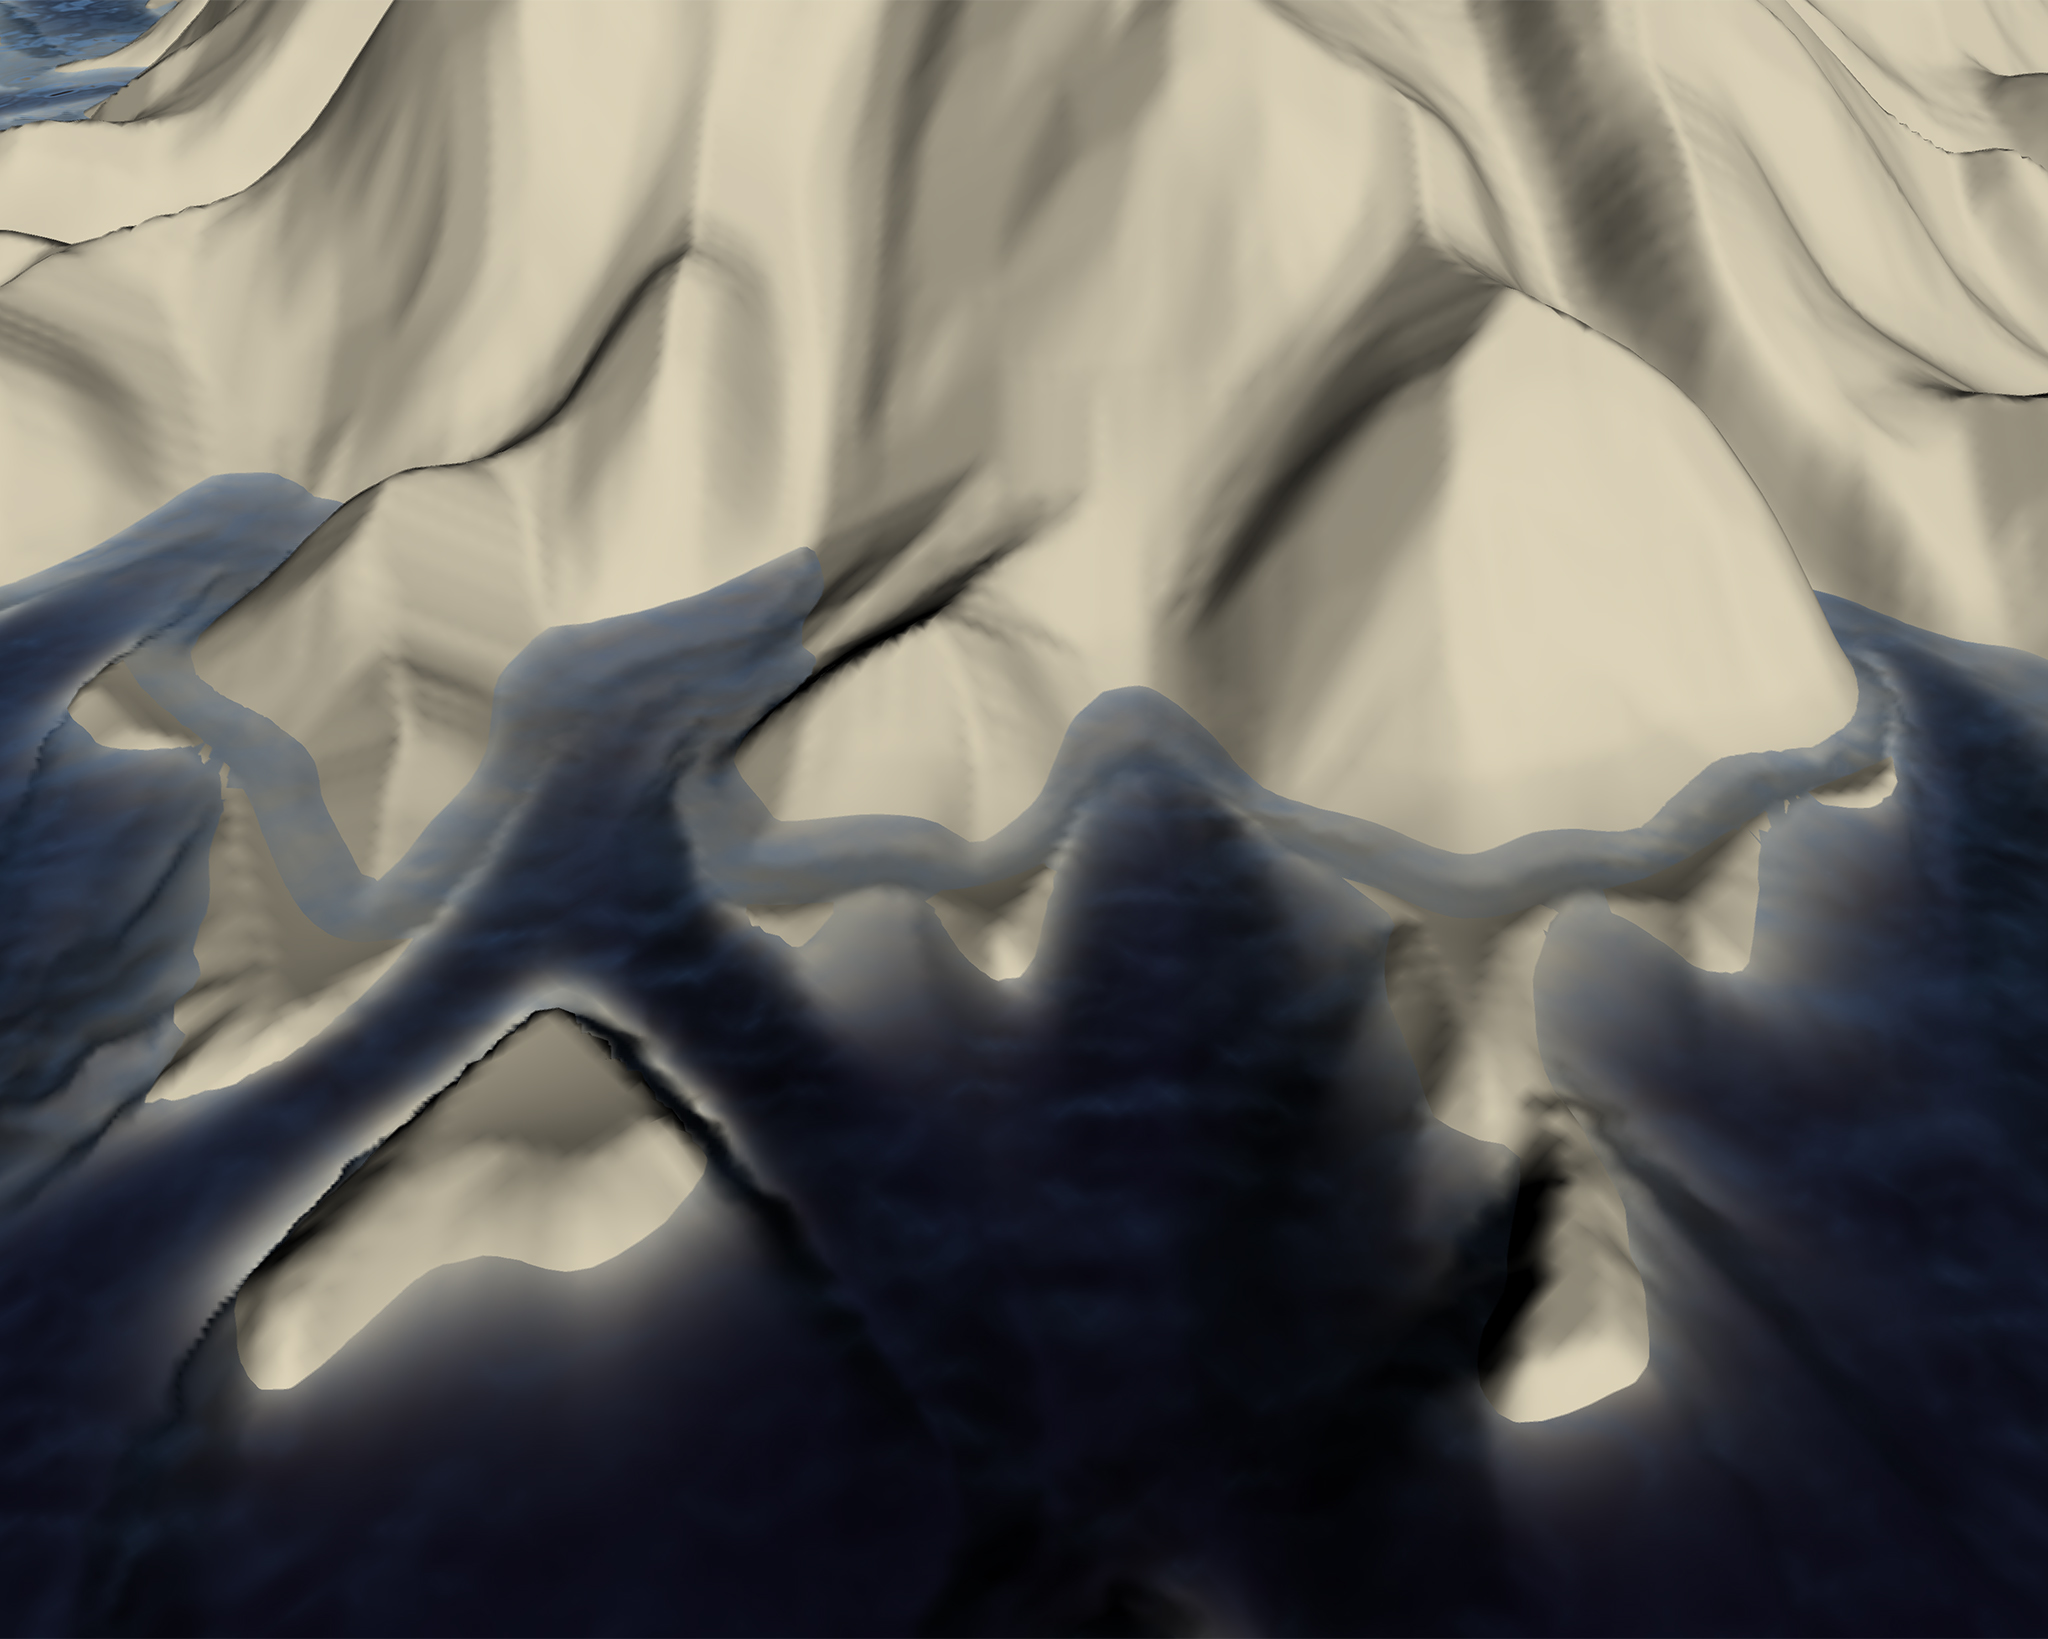
\includegraphics[width=0.25\linewidth]{example_coral_reef}%
    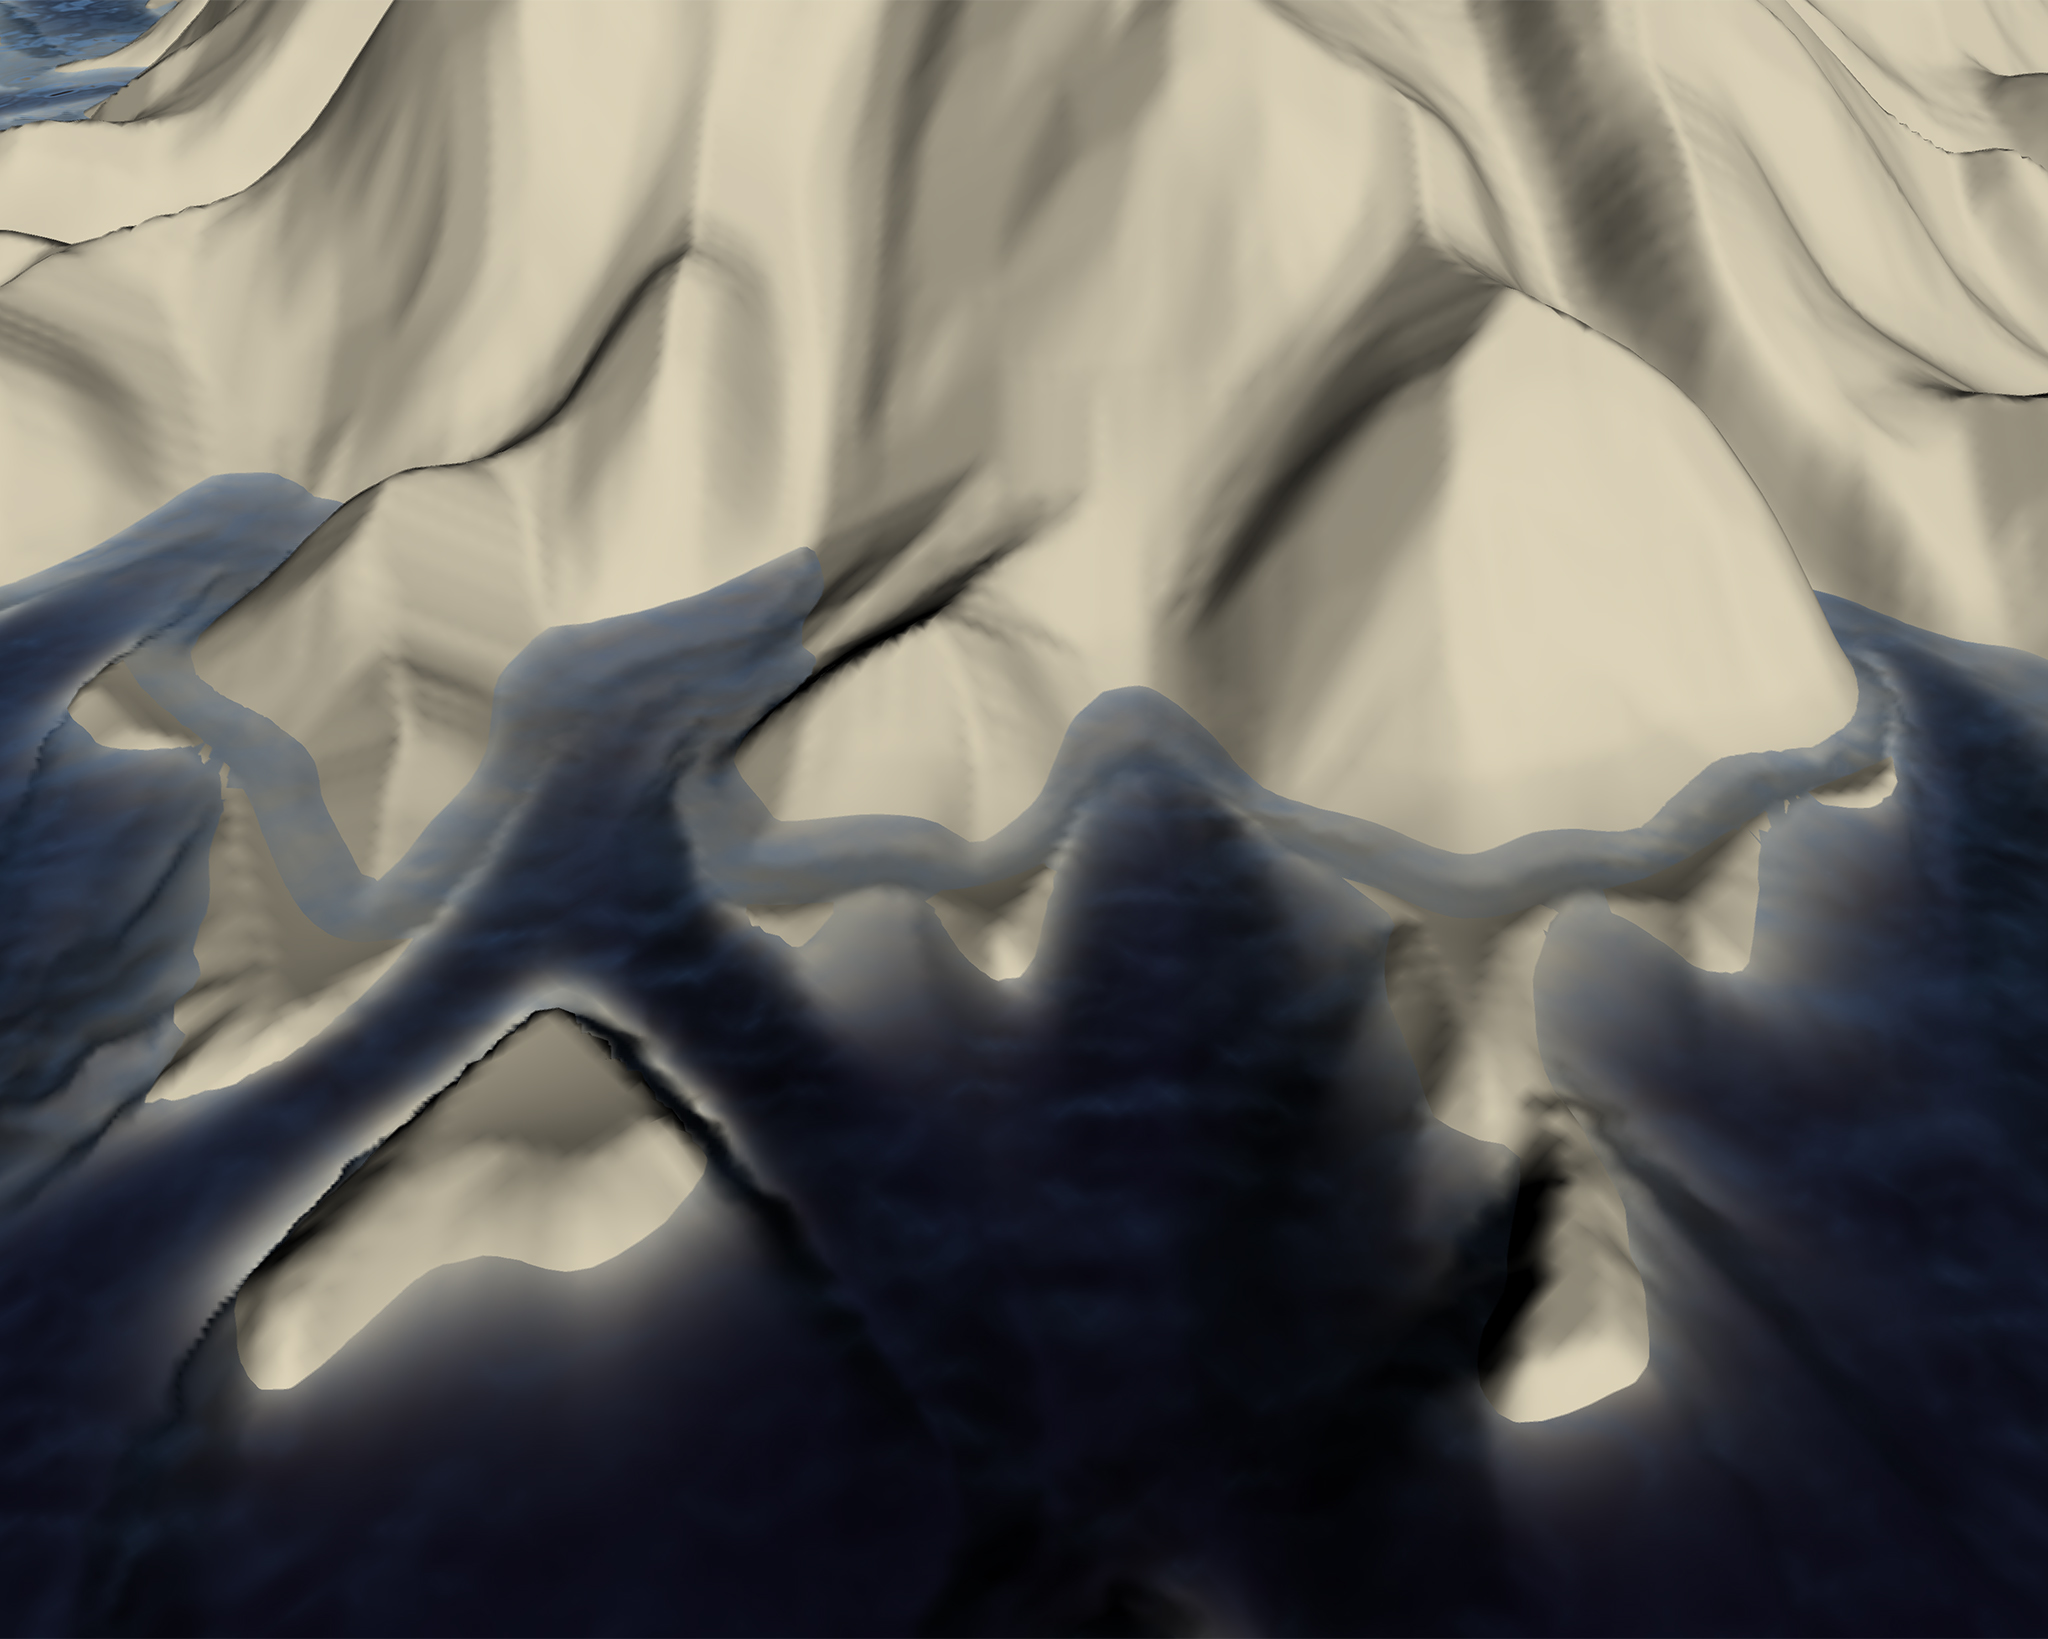
\includegraphics[width=0.25\linewidth]{example_coral_reef}%
    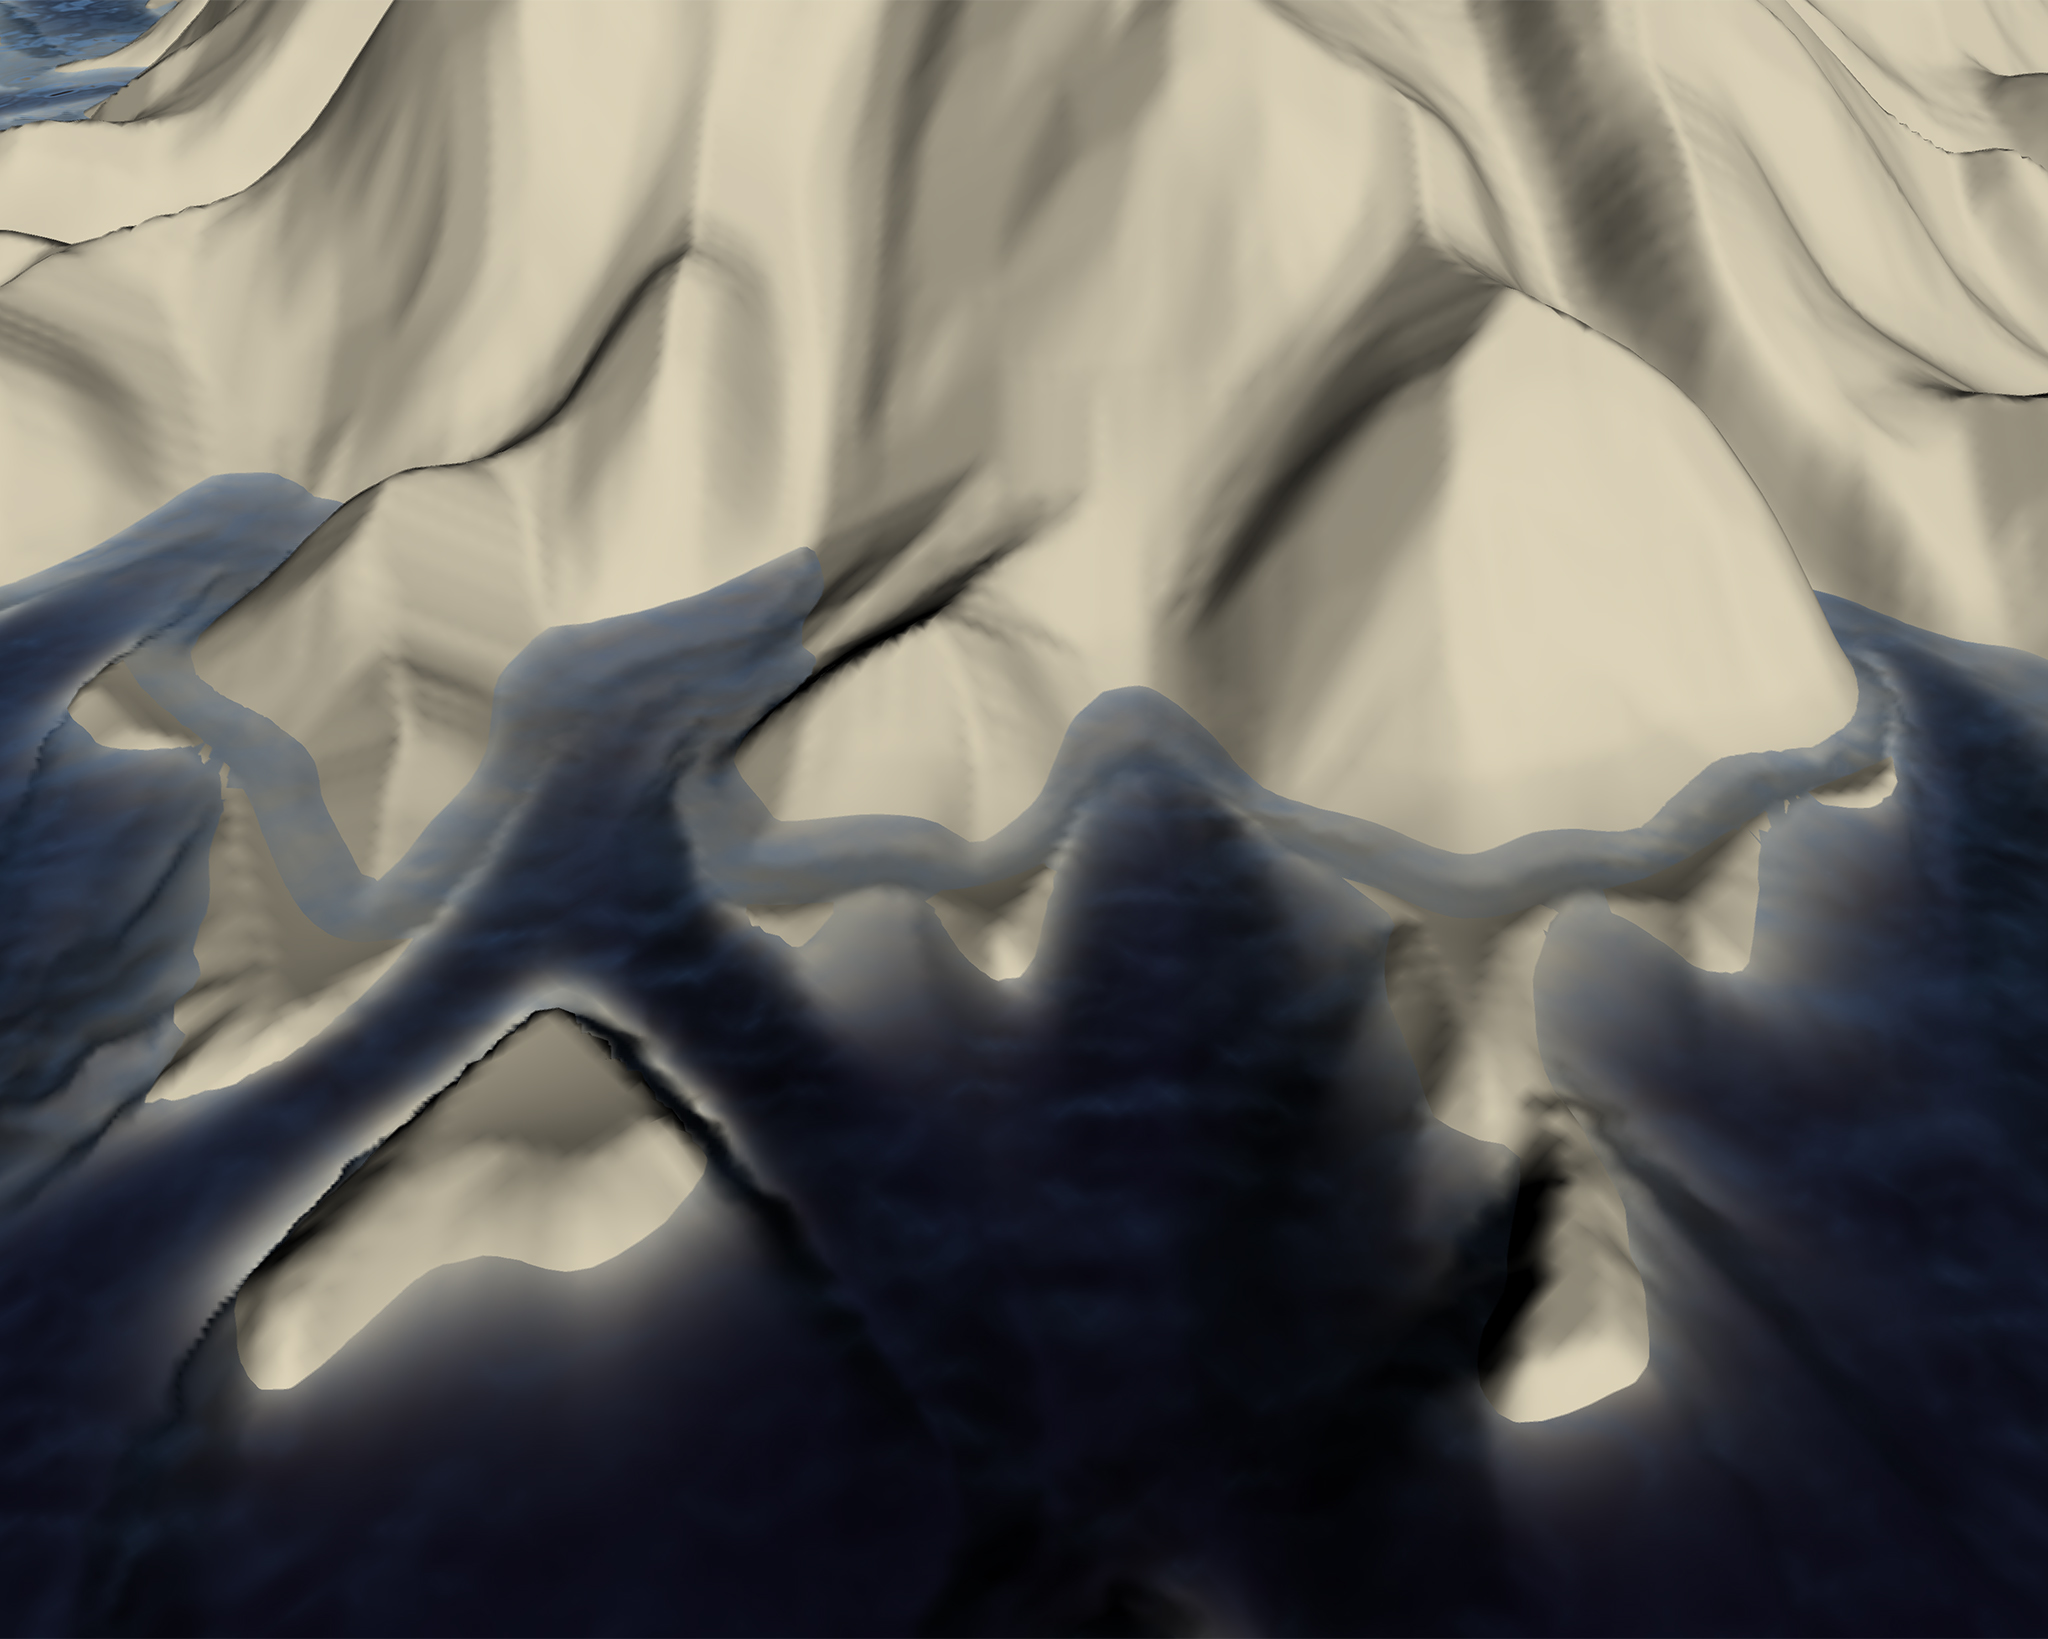
\includegraphics[width=0.25\linewidth]{example_coral_reef}\\%
    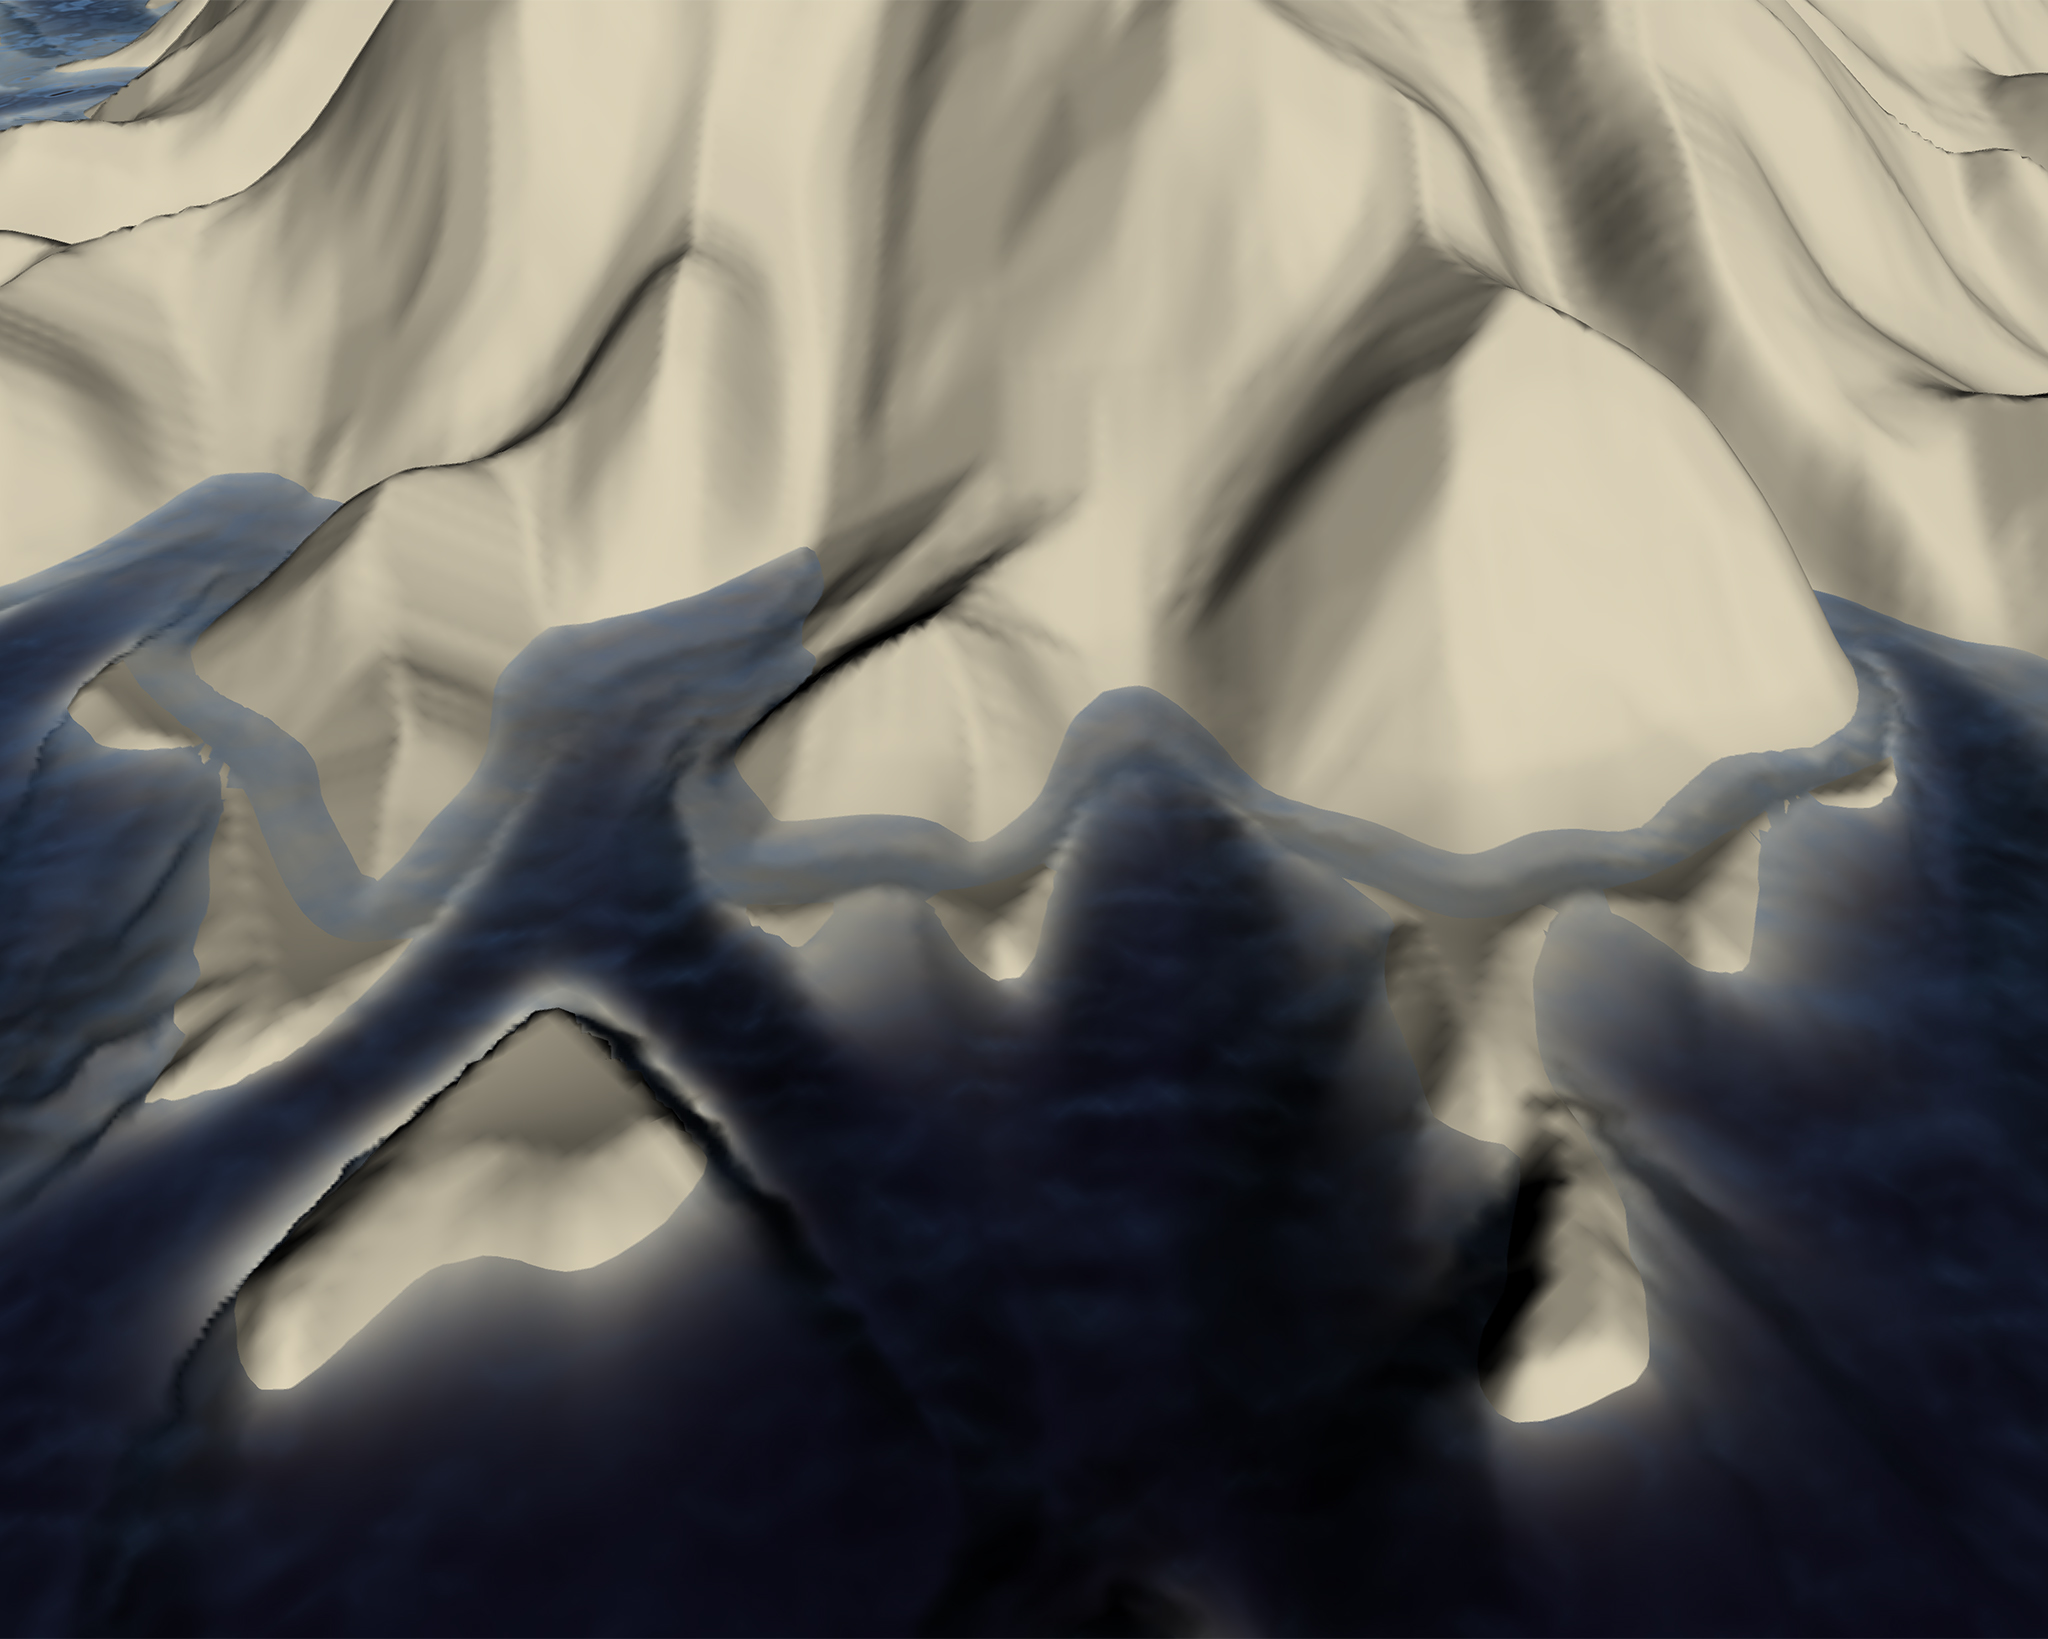
\includegraphics[width=0.25\linewidth]{example_coral_reef}%
    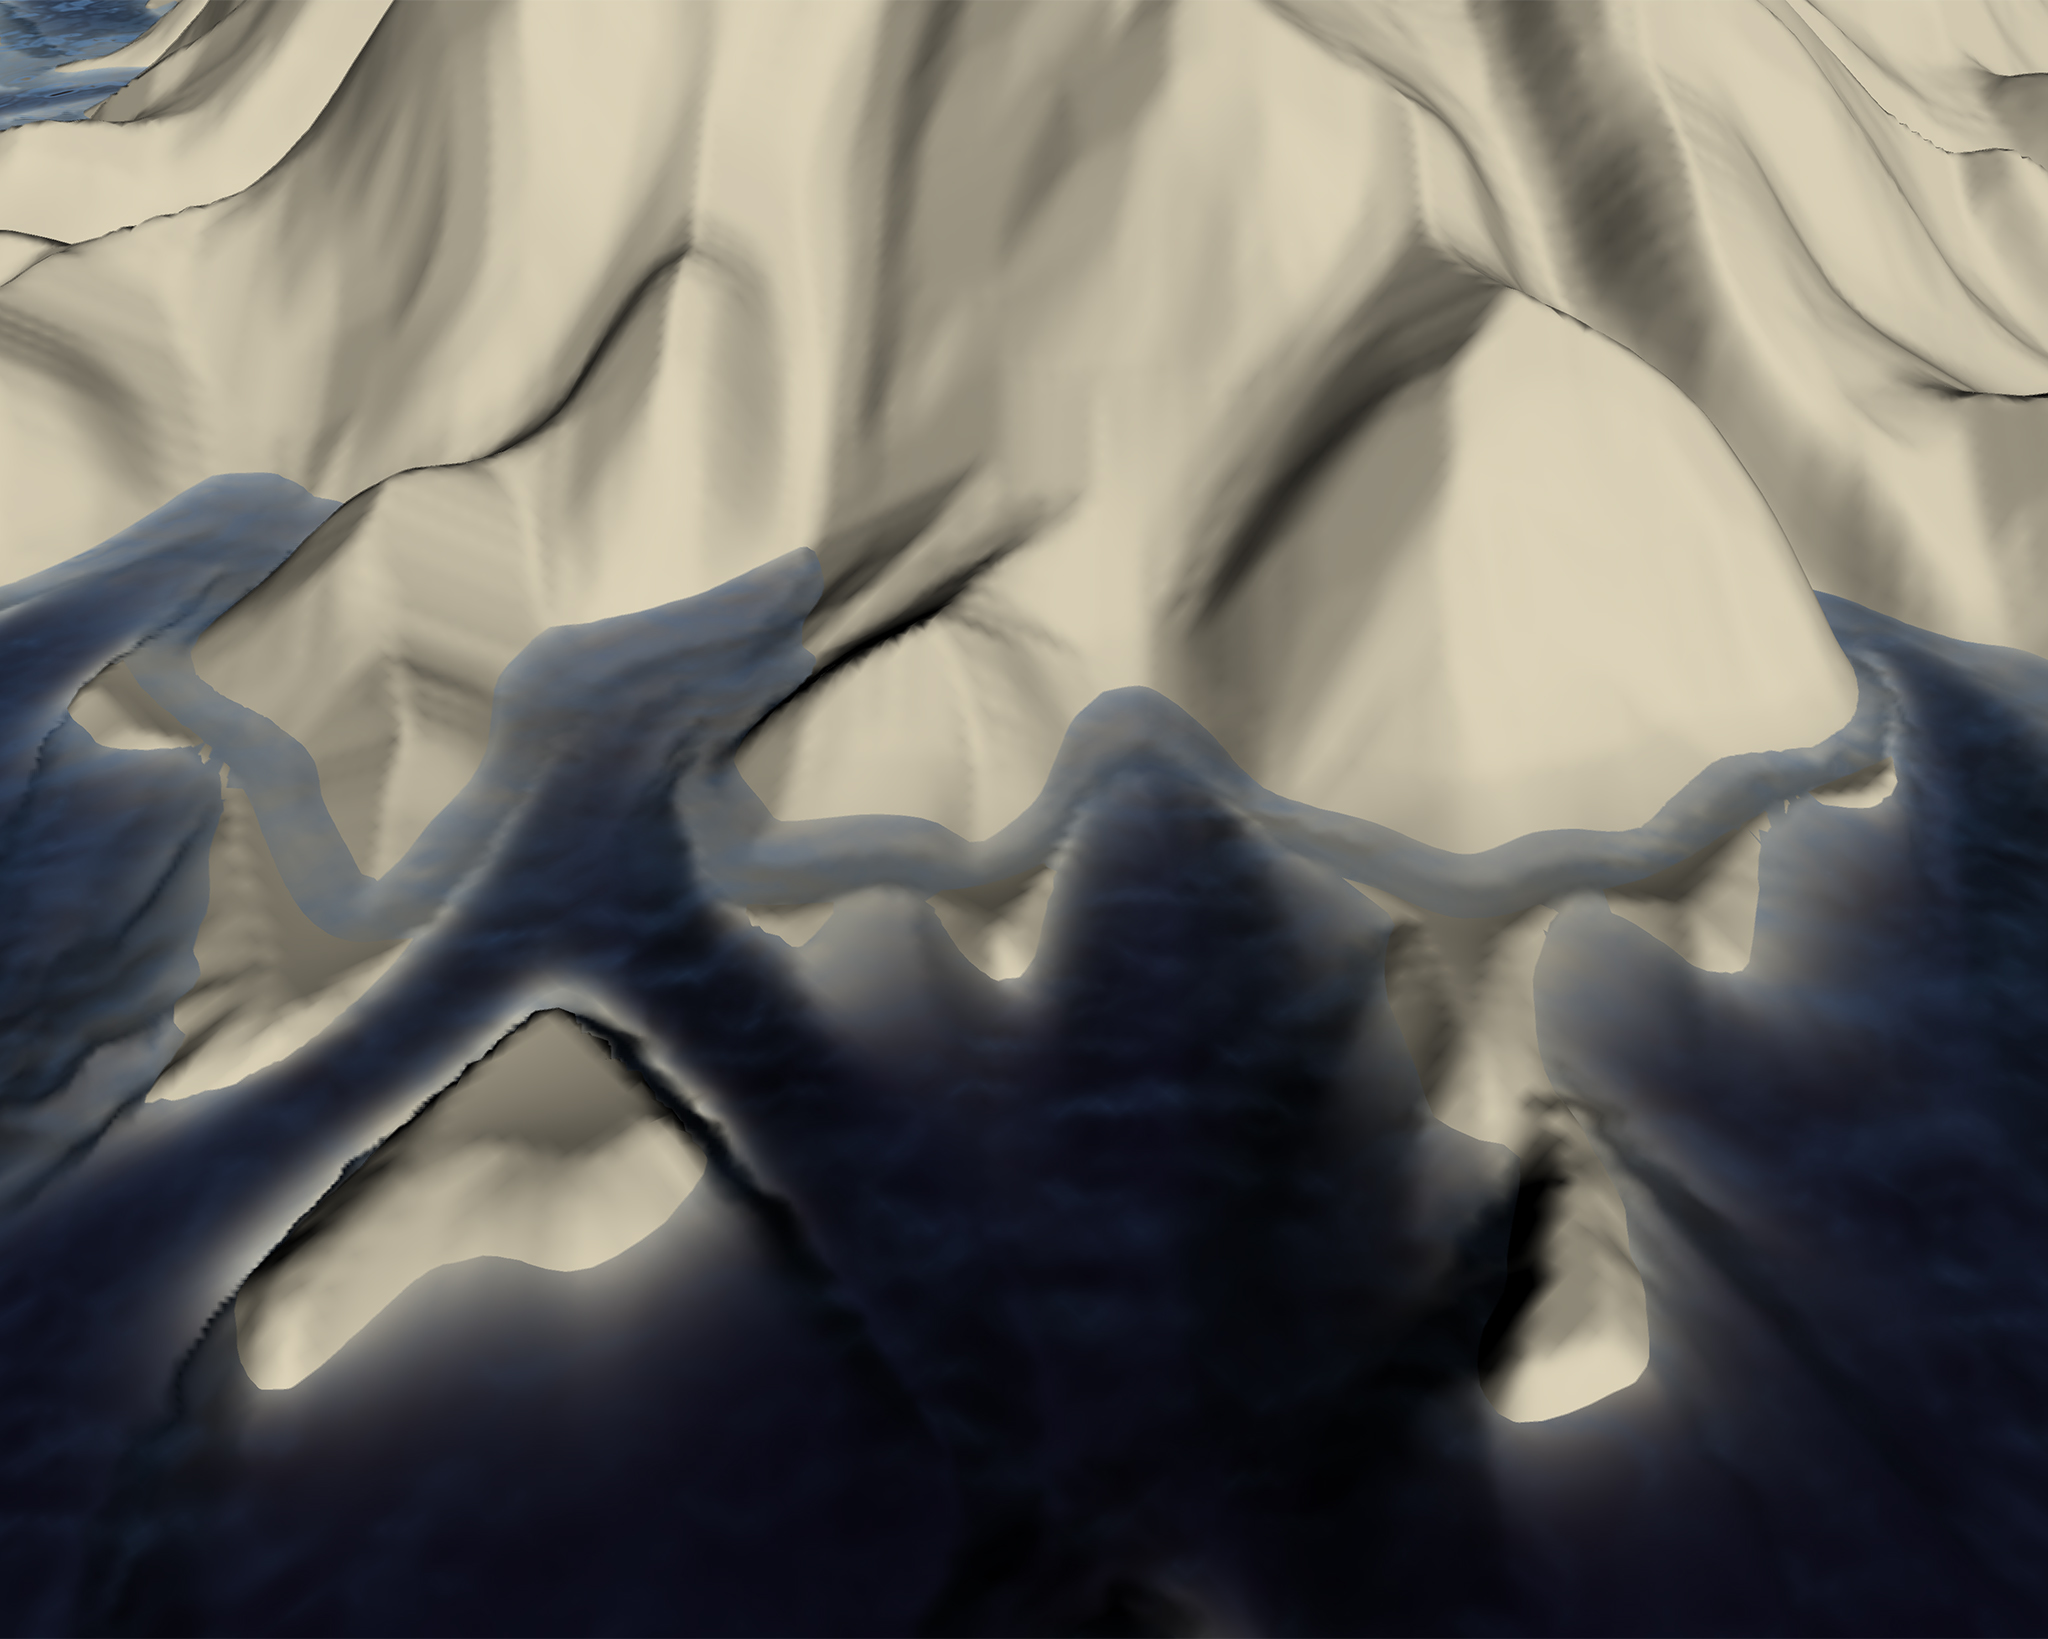
\includegraphics[width=0.25\linewidth]{example_coral_reef}%
    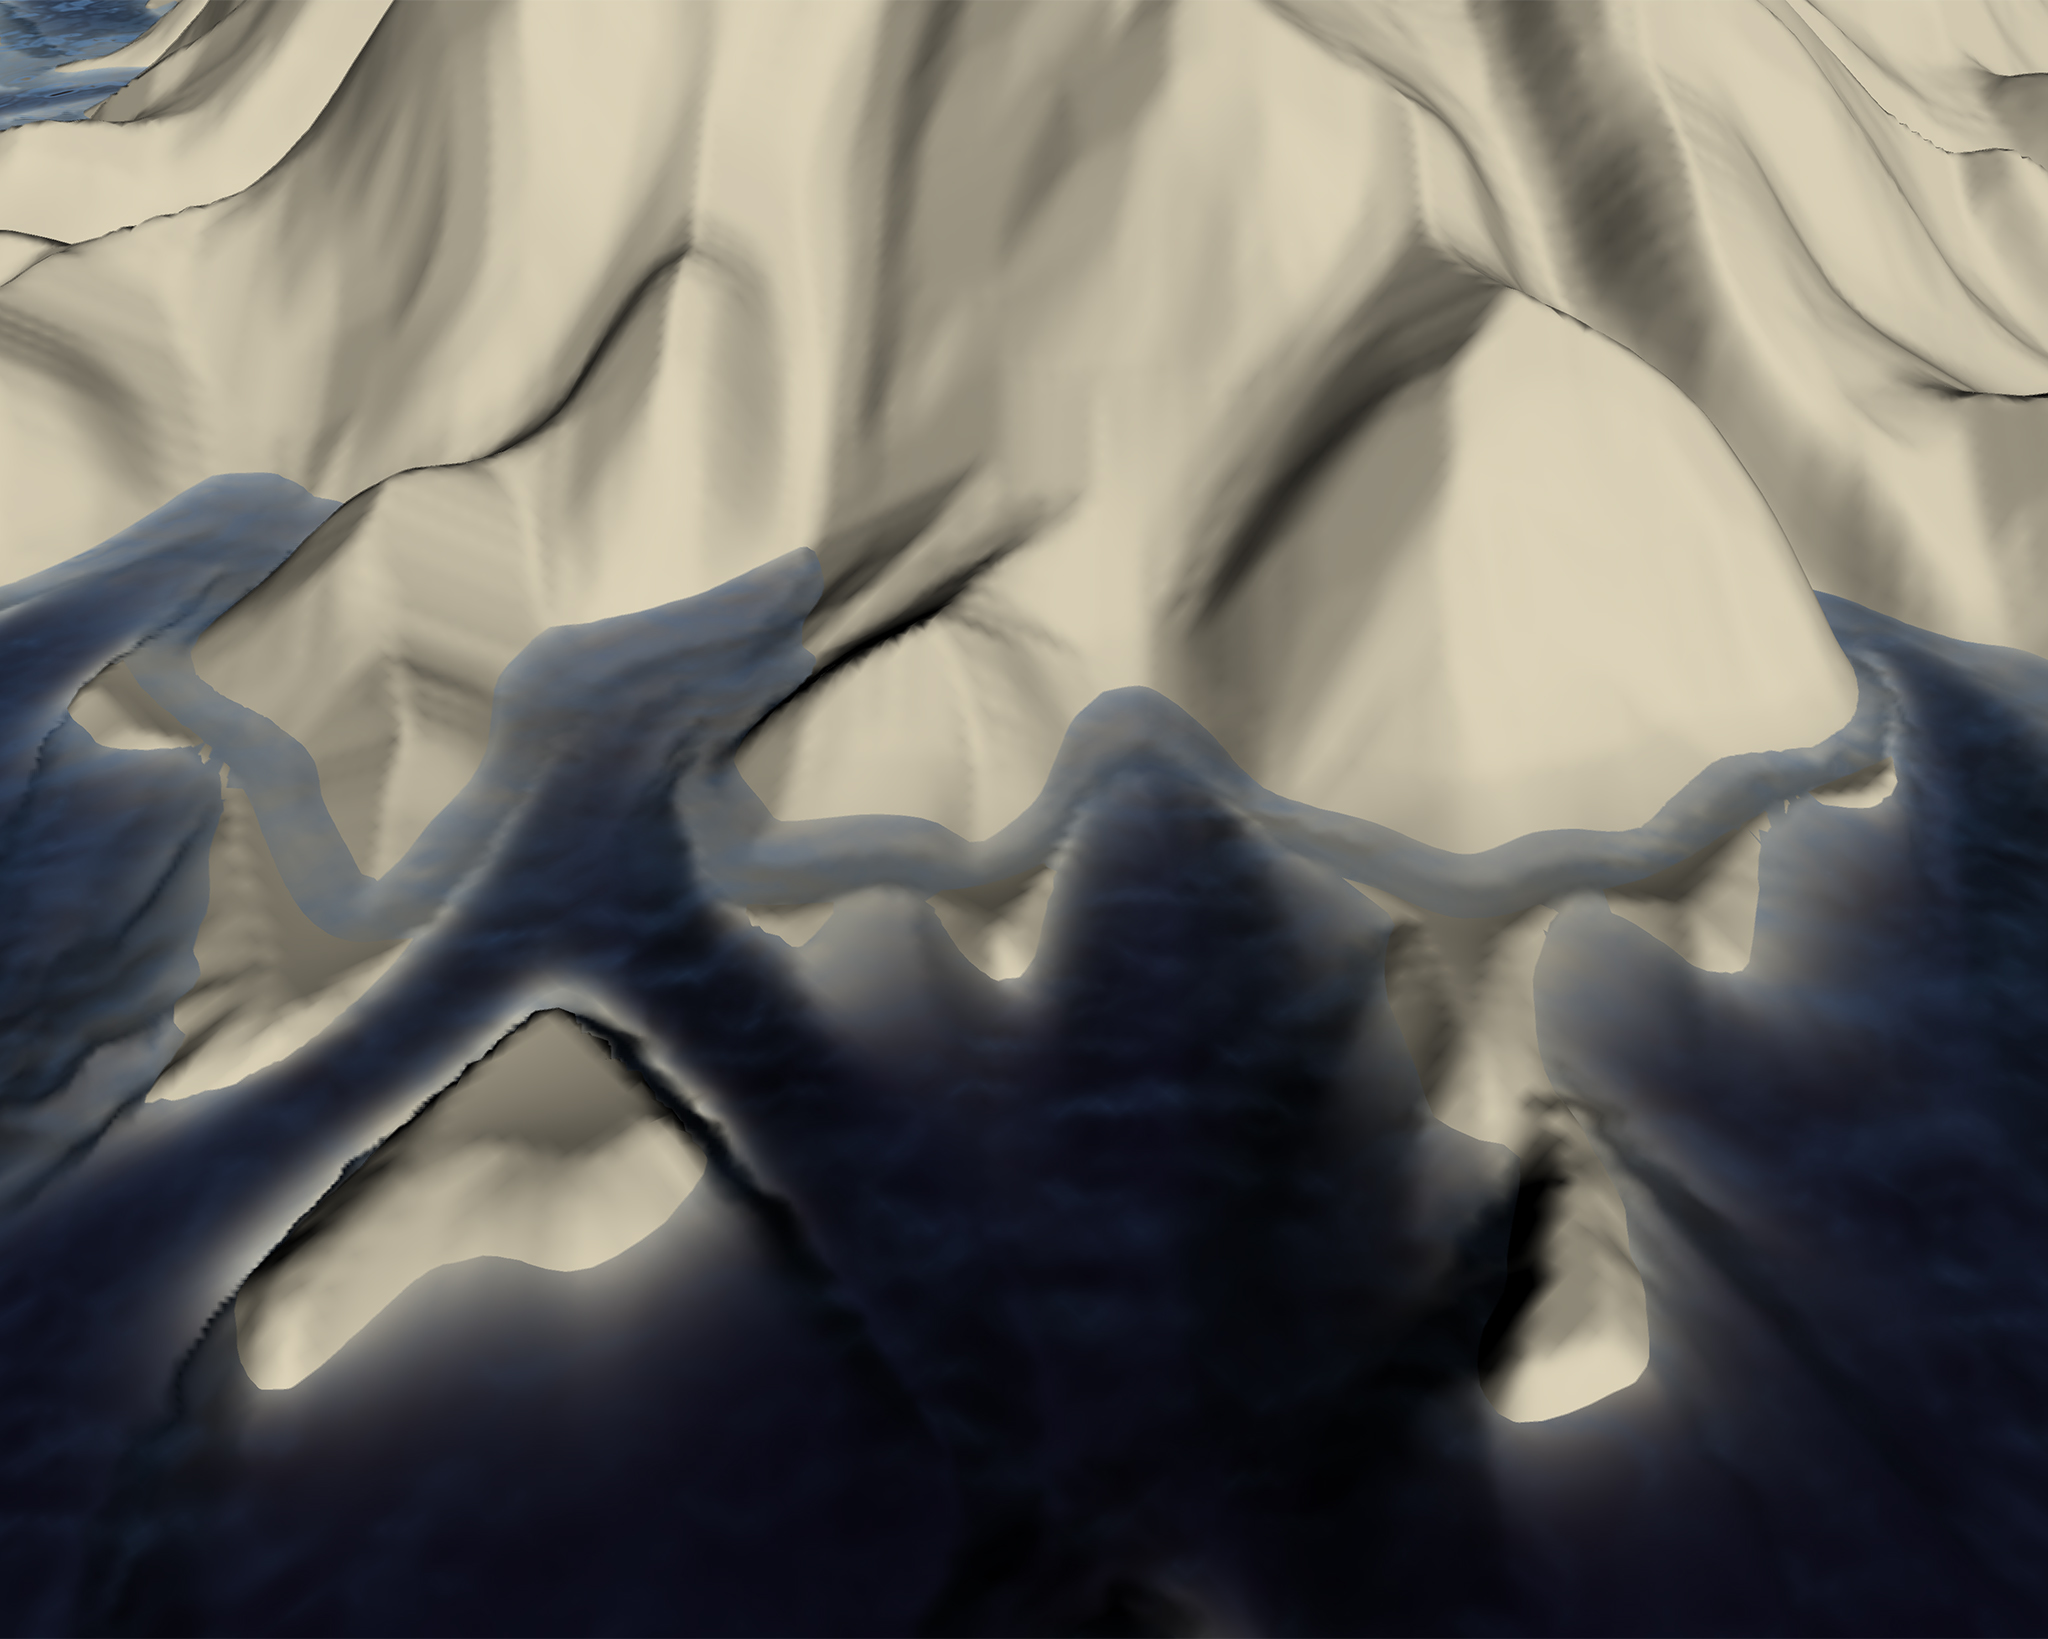
\includegraphics[width=0.25\linewidth]{example_coral_reef}%
    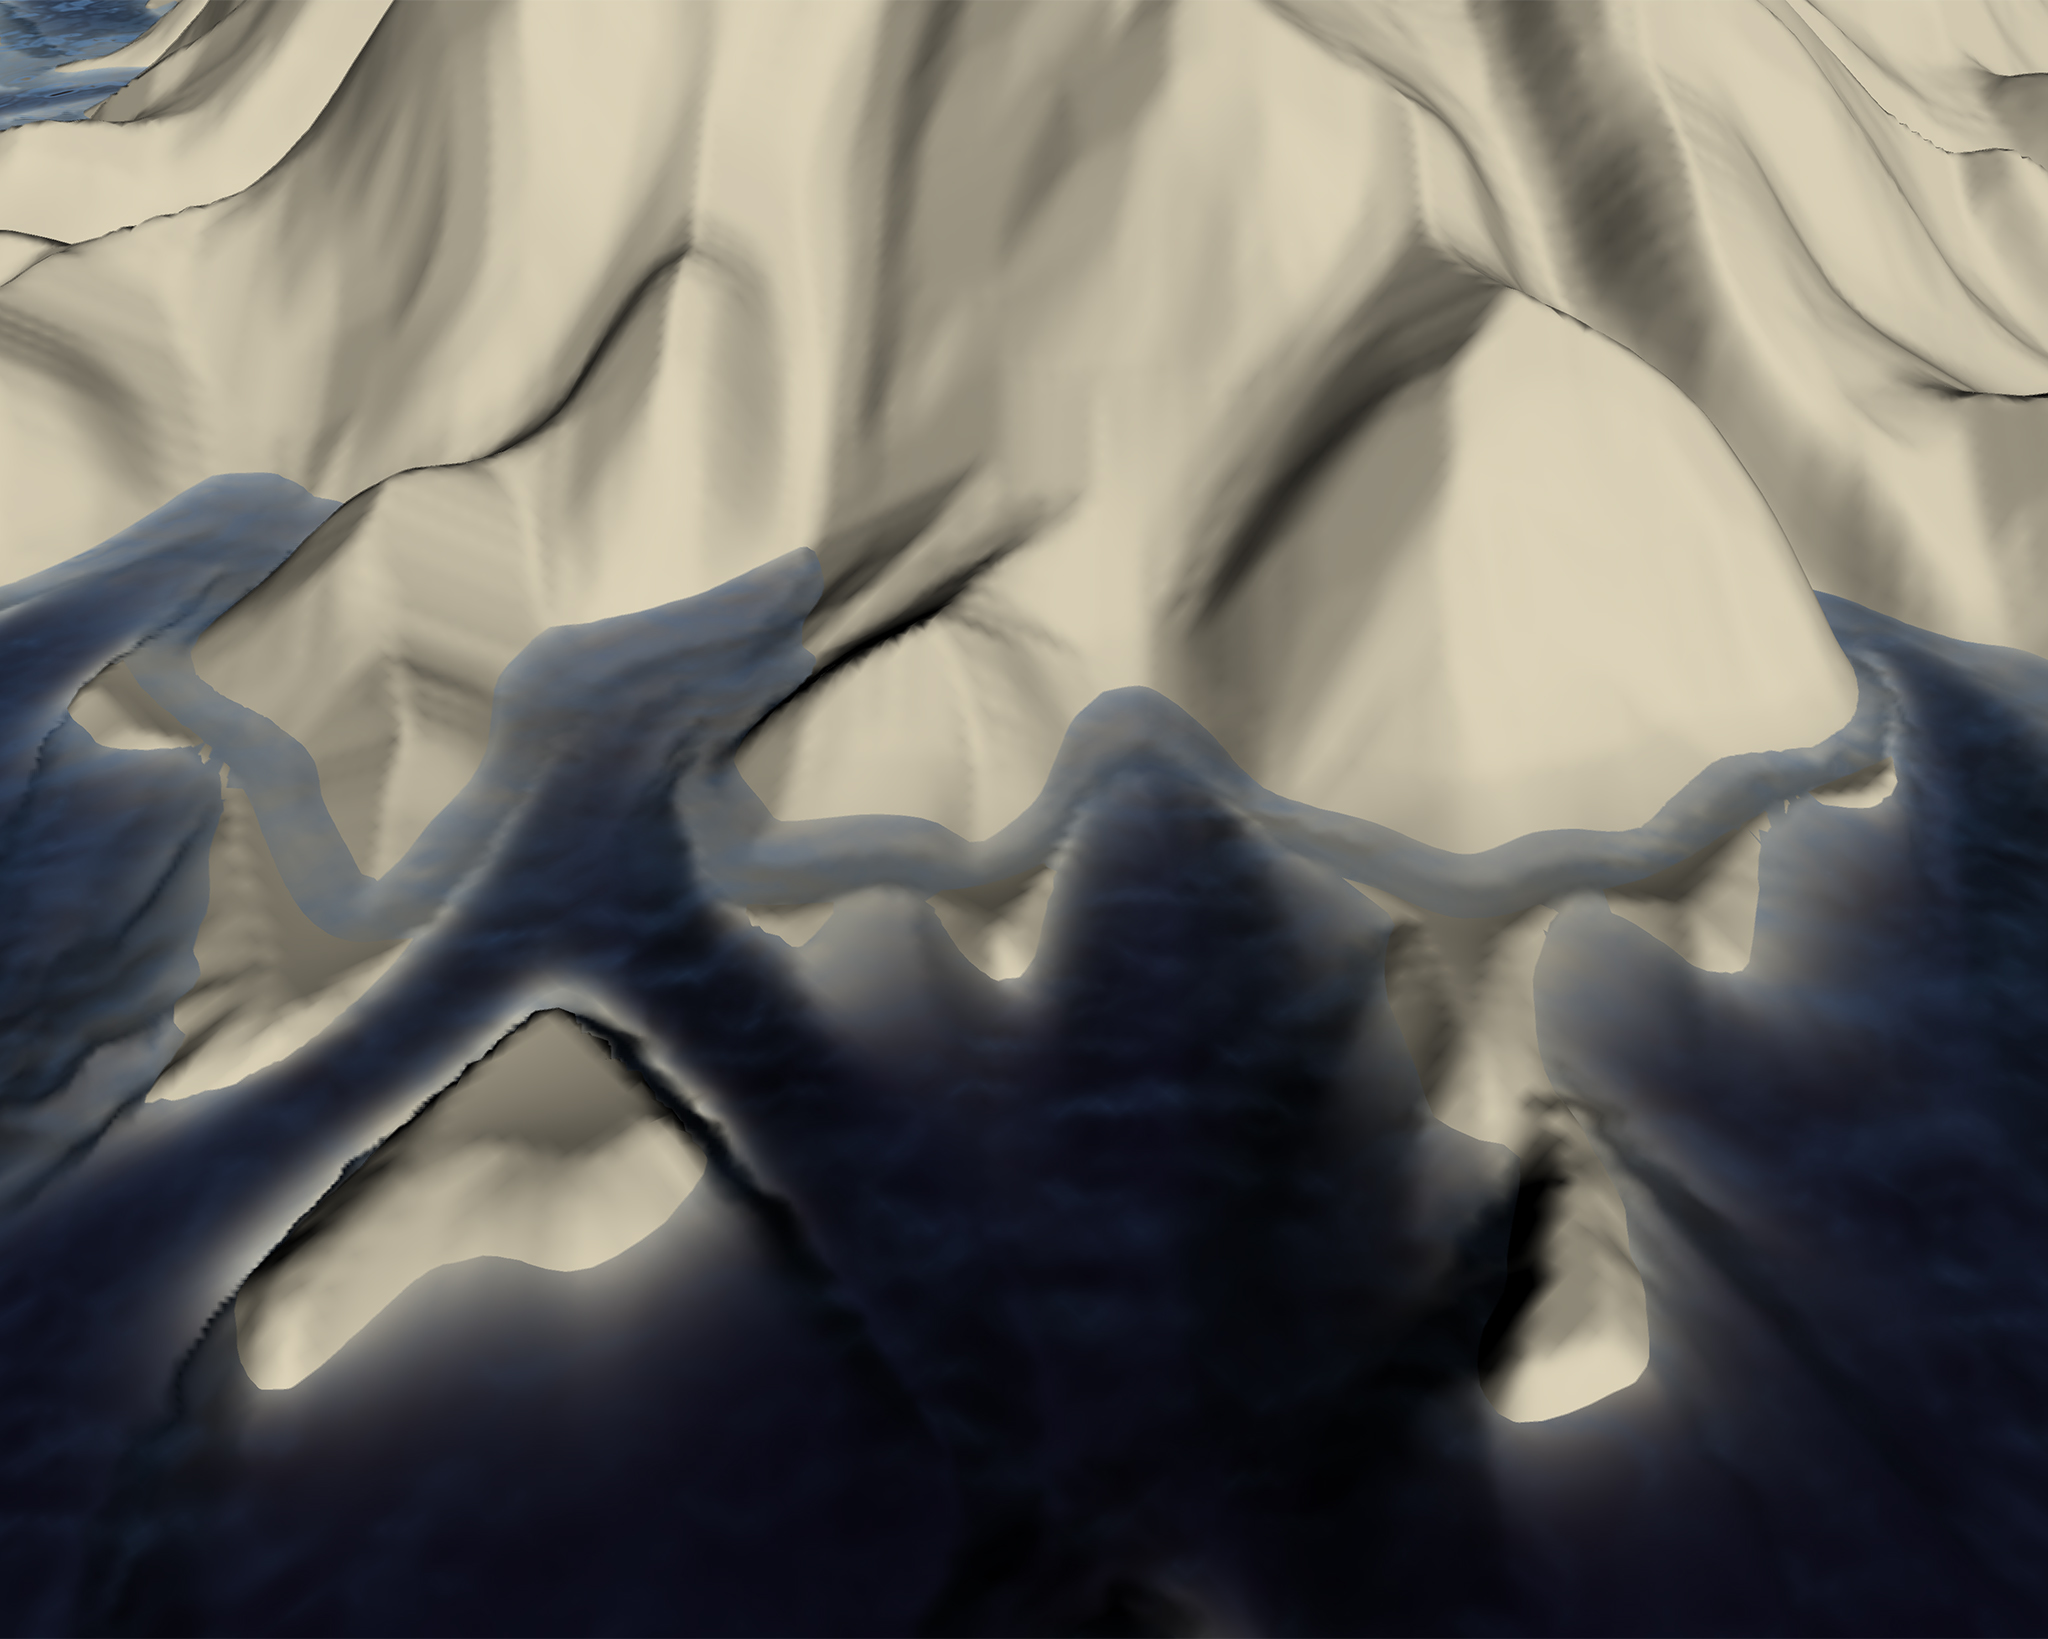
\includegraphics[width=0.25\linewidth]{example_coral_reef}%
    }
    \caption{Mreža osmih slik brez vmesnih presledkov in z le enim skupnim naslovom. Vključena je tudi širša postavitev.}
    \label{sl:mreza_4x2_brez_presledkov}
\end{largefigure}

\subsubsection{Več tabel ena ob drugi}

Logika postavljanja dveh tabel ene ob drugo je popolnoma enaka kot pri slikah, le da znotraj okolja \ltx|table| uporabimo okolje \ltx|subtable|. Edino pomembno pravilo, na katerega ne smete pozabiti, je: \textbf{podnaslovi tabel vedno sodijo nad tabelo}, medtem ko podnaslovi slik sodijo pod njo. 

Če ugotovite, da je vsebina tabele preširoka in povzroča prekrivanje, lahko celotno okolje \ltx|tabular| ovijete v ukaz \ltx|\resizebox{\ linewidth}{!}{...}|, ki tabelo proporcionalno pomanjša, da se natančno prilega širini podtabele. Tabela~\ref{tab:rezultati_cv} prikazuje ustrezen zapis na primeru vrednotenja modelov računalniškega vida.

\begin{table}[htbp]
    \centering
    \caption{Primerjava uspešnosti klasifikacije slik z različnimi arhitekturami globokih nevronskih mrež na dveh standardnih podatkovnih zbirkah. Pri metriki \textit{točnost} (angl.\ \textit{accuracy}) so boljše višje vrednosti (označeno s puščico $\uparrow$), pri metriki \textit{napaka} (angl.\ \textit{error rate}) pa so boljše nižje vrednosti (označeno s puščico $\downarrow$).}
    \label{tab:rezultati_cv}
    \begin{subtable}[b]{0.48\textwidth}
        \centering
        \caption{Rezultati na zbirki CIFAR-10.}
        \label{tab:cifar10}
        \resizebox{\linewidth}{!}{%
        \begin{tabular}{lcc}
            \hline
            arhitektura & točnost ($\uparrow$) & napaka ($\downarrow$) \\
            \hline
            ResNet-18 & 93,5 \% & 6,5 \% \\
            ResNet-50 & 95,2 \% & 4,8 \% \\
            ViT-Base  & 97,8 \% & 2,2 \% \\
            \hline
        \end{tabular}%
        }
    \end{subtable}
    \hfill
    \begin{subtable}[b]{0.48\textwidth}
        \centering
        \caption{Rezultati na zbirki ImageNet.}
        \label{tab:imagenet}
        \resizebox{\linewidth}{!}{%
        \begin{tabular}{lcc}
            \hline
            arhitektura & točnost ($\uparrow$) & napaka ($\downarrow$) \\
            \hline
            ResNet-18 & 69,7 \% & 30,3 \% \\
            ResNet-50 & 76,1 \% & 23,9 \% \\
            ViT-Base  & 84,2 \% & 15,8 \% \\
            \hline
        \end{tabular}%
        }
    \end{subtable}
\end{table}

Omogočena je tudi uporaba širokih tabel, kot vidimo iz tabele~\ref{tab:large}.

\begin{largetable}[t]
    \caption{Primer široke tabele. Prikazani so časi izvajanja treh namišljenih algoritmov. Razvidno je, da ima algoritem A eksponentno časovno zahtevnost, algoritem B kvadratno časovno zahtevnost in algoritem C linearno časovno zahtevnost. Tovrstne podatke je sicer bolj smiselno prikazovati na grafu, a za demonstracijo uporabe široke tabele bi moralo zadoščati.}
    \label{tab:large}
    \begin{tabular}{*{4}{p{\dimexpr(\linewidth-8\tabcolsep)/4\relax}}}
    $n$ & čas izvajanja algoritma A & čas izvajanja algoritma B & čas izvajanja algoritma C \\\hline
    5 & \SI{2}{\second} & \SI{3}{\second} & \SI{4}{\second}\\
    10 & \SI{61}{\second} & \SI{9}{\second} & \SI{6}{\second}\\
    15 & \SI{33}{\minute} & \SI{18}{\second} & \SI{8}{\second}\\
    20 & \SI{17}{\hour} & \SI{32}{\second} & \SI{10}{\second}\\\hline
    \end{tabular}
\end{largetable}

\section{Vključevanje programske kode in algoritmov}
\label{sec:koda}

Svojo programsko kodo v poljubnem programskem jeziku najlažje vključimo s paketom \ltx|minted|. Okoli bloka \ltx|\minted{ }| sicer lahko podamo klasični \ltx|\listing{ }| in skupaj z dodanim \ltx|\caption| dobimo vse potrebno za prikaz kode, vendar pa se takšen blok ne razteza pravilno skozi več strani. Ena od možnosti za rešitev je uporaba bloka \ltx|\center{ }|, za napis pa \ltx|\captionof{ }|, kot je prikazano pri obeh primerih izsekov kode~\ref{code:py} in~\ref{code:js}.

\begin{center}
\captionsetup{hypcap=false}
\captionof{listing}{Kratek primer kode v programskem jeziku Python.}
\label{code:py}
\begin{minted}{python}
def python_veverica():
    # Oh, kako je to lepo!
    x = -1
    print("Res izgleda čudovito.")
\end{minted}
\end{center}

Kar je nadvse čudovito pri paketu \ltx|minted| je to, da lahko podamo dele kode znotraj vrstice, kot je npr. tole: \mintinline{python}{python_veverica()}.

\begin{center}
\captionsetup{hypcap=false}
\captionof{listing}{Malo daljši primer programske kode v jeziku Javascript, ki se lahko razteza skozi dve strani.}
\label{code:js}
\begin{minted}{javascript}
async function pridobiUporabnika(id) {
    const url = `https://api.primer.fri/users/${id}`;
    
    try {
        const odgovor = await fetch(url);
        
        // Preverimo, če je statusni kod v območju 200-299
        if (!odgovor.ok) {
            console.error(`Napaka pri povezavi: ${odgovor.status}`);
            throw new Error(`Uporabnika z ID ${id} ni bilo mogoče najti.`);
        }

        const podatki = await odgovor.json();
        
        // Logiranje uspešnega prejema podatkov
        console.log("Podatki so bili uspešno prejeti.");
        console.log(`Ime uporabnika: ${podatki.name}`);
        
        return podatki;
        
    } catch (napaka) {
        // Tukaj ulovimo tako mrežne napake kot napake pri branju JSON-a
        console.warn("Prišlo je do nepričakovane težave.");
        return { error: napaka.message };
    }
}
\end{minted}
\end{center}

Vodoravni črti pri začetku in koncu izseka, v kombinaciji s sivim ozadjem, vizualno sporočata morebitno raztezanje skozi več strani. To je razvidno pri izseku kode~\ref{code:js}.

\subsection{Vključevanje algoritmov (psevdokode)}

Medtem ko paket \ltx|minted| uporabljamo za prikaz dejanske implementacije v specifičnem programskem jeziku, v zaključnih delih pogosto opisujemo samo logiko reševanja problema na višjem nivoju. Za zapis algoritmov v obliki psevdokode je standardna izbira kombinacija paketov \ltx|algorithm| in \ltx|algpseudocode| (slednji je del paketa \ltx|algorithmicx|).

Za razliko od izsekov izvorne kode, algoritme običajno obravnavamo kot standardne plavajoče objekte (tako kot slike in tabele). To pomeni, da \LaTeX\ sam poišče optimalno mesto za njihov prikaz na strani. V besedilu se nanje sklicujemo z nedeljivim presledkom in ukazom \ltx|\ref|, na primer: Algoritem~\ref{alg:evklid} prikazuje klasičen postopek za iskanje največjega skupnega delitelja.

Naslov (\ltx|\caption|) pri algoritmih običajno postavljamo na vrh, tik pod začetek okolja \ltx|algorithm|. Številka \ltx|[1]| ob začetku bloka \ltx|algortihmic| pa \LaTeX u sporoči, naj oštevilči vsako vrstico algoritma, kar nam olajša sklicevanje na posamezne korake v besedilu.

\begin{algorithm}[htbp]
\caption{Evklidov algoritem za iskanje največjega skupnega delitelja}
\label{alg:evklid}
\begin{algorithmic}[1] 
    \Require $a \geq 0 \lor b \geq 0$ % Vhodni pogoji
    \Ensure Največji skupni delitelj $a$ in $b$ % Izhod
    \Statex % Prazna vrstica za boljšo preglednost
    \Procedure{Evklid}{$a, b$}
        \While{$b \neq 0$}
            \State $t \gets b$
            \State $b \gets a \bmod b$
            \State $a \gets t$
        \EndWhile
        \State \textbf{return} $a$
    \EndProcedure
\end{algorithmic}
\end{algorithm}

\section{Matematično okolje in sklicevanje na besedilne konstrukte}
\label{sec:mat}

Poglejmo nekaj primerov pisanja enačb, sklicevanj nanje, podajanja dokazov, matrik, razbijanje enačb in nekaj splošnih tipografskih pravil v matematiki.
\begin{theorem}
  \label{iz:1}
  Za vsako naravno število $n$ velja
  \begin{equation}
    n < 2^n.
    \label{eq:1}
  \end{equation}
\end{theorem}

\begin{proof}
  Dokazovanje z indukcijo zahteva, da neenakost~\eqref{eq:1} najprej preverimo za najmanjše naravno število -- $0$.
  Res, ker je $0 < 1 = 2^0$, je neenačba~\eqref{eq:1} za $n=0$ izpolnjena.

  Enačbo~\eqref{eq:1} smo referencirali z \ltx|~\eqref{eq:1}| in ne z \ltx|~\ref{eq:1}|, saj nam slednji ne ovije reference v oklepaje. Brez oklepajev bi bralec lahko referenco na enačbo zamenjal z referenco na razdelek, z oglatimi oklepaji pa na sklic v literaturi.
  
  Za potrebe primera nadaljujmo z indukcijskim korakom. S predpostavko, da je neenakost~\eqref{eq:1} veljavna pri nekem naravnem številu $n$, je potrebno pokazati, da je ista neenakost v veljavi tudi pri njegovem nasledniku -- naravnem številu $n+1$.
  Računajmo.
  \begin{align}
    n+1 & < 2^n + 1       \label{eq:2}\\
    & \le 2^n + 2^n \label{eq:3}\\
    & = 2^{n+1}       \nonumber
  \end{align}
  Neenakost~\eqref{eq:2} je posledica indukcijske predpostavke, neenakost~\eqref{eq:3} pa enostavno dejstvo, da je za vsako naravno število $n$ izraz $2^n$ vsaj tako velik kot 1.
  S tem je dokaz Izreka~\ref{iz:1} zaključen.
\end{proof}

Ste opazili kako so indukcijski koraki lepo poravnani? Uporabili smo pomemben \ltx|align|. Ste opazili, da smo stavek pri neenakosti~\ref{eq:1} končali s piko? V primeru, da je enačba del povedi, kot npr.
 \begin{equation}
    y = 2^x,
    \label{eq:1b}
  \end{equation}
pa seveda dodamo vejico v samo enačbo, kot je prikazno pri~\eqref{eq:1b}. 
% Sledi pa še en primer z zares dolgo enačbo, ki se razteza skozi celotno širino, kot je prikazano pri enačbi~\eqref{eq:2}.

% \begin{widetext}
% \begin{equation*}
%     \mathcal{L}_{\text{SM}} = -\frac{1}{4} G_{\mu\nu}^a G_a^{\mu\nu} - \frac{1}{4} W_{\mu\nu}^i W_i^{\mu\nu} - \frac{1}{4} B_{\mu\nu} B^{\mu\nu} + \sum_{\psi=L,Q} \bar{\psi} i \gamma^\mu D_\mu \psi + \sum_{\psi=e,u,d} \bar{\psi} i \gamma^\mu D_\mu \psi + (D_\mu \phi)^\dagger (D^\mu \phi) - \mu^2 \phi^\dagger \phi - \lambda (\phi^\dagger \phi)^2 - \left( \bar{L} Y_e \phi e_R + \bar{Q} Y_u \tilde{\phi} u_R + \bar{Q} Y_d \phi d_R + \text{h.c.} \right)
%   \label{eq:2}
% \end{equation*}
% \end{widetext}

Za kakovostno tehnično pisanje pa moramo obvladati še zapis matrik in obdelavo zelo dolgih enačb.

\subsection{Matrike}

Za zapis matrik uporabljamo okolja iz paketa \ltx|amsmath|. Najpogosteje uporabljamo okolje \ltx|bmatrix| za matrike z oglatimi oklepaji ali \ltx|pmatrix| za matrike z okroglimi oklepaji.

Primer zapisa matrike $A$:
\begin{equation}
    A = \begin{bmatrix}
        a_{11} & a_{12} & \dots  & a_{1n} \\
        a_{21} & a_{22} & \dots  & a_{2n} \\
        \vdots & \vdots & \ddots & \vdots \\
        a_{m1} & a_{m2} & \dots  & a_{mn}
    \end{bmatrix}.
\end{equation}

Pri tem elemente v vrstici ločimo z znakom \ltx|\&|, vrstice pa zaključimo z \ltx|\\|. Za različne vrste pik uporabljamo ukaze \ltx|\dots| (vodoravne), \ltx|\vdots| (navpične) in \ltx|\ddots| (diagonalne).

\subsection{Razbijanje dolgih enačb}

Kadar je enačba predolga za eno vrstico, uporabimo okolje \ltx|split| znotraj okolja \ltx|equation|. To nam omogoča, da enačbo razbijemo na several vrstic, medtem ko celoten blok obdrži le eno skupno številko.

\begin{equation}
    \begin{split}
        f(x) &= (a+b)^4 \\
             &= a^4 + 4a^3b + 6a^2b^2 + 4ab^3 + b^4.
    \end{split}
    \label{eq:razcep}
\end{equation}

Znak \ltx|\&| določa točko poravnave (običajno pri enačaju), \ltx|\\| pa prehod v novo vrstico.

\subsection{Sistemi enačb in primeri}

Za zapis funkcij, ki so definirane po delih, ali za sisteme enačb z enim velikim oklepajem uporabljamo okolje \ltx|cases|:

\begin{equation}
    |x| = \begin{cases}
        x,  & \text{če je } x \ge 0, \\
        -x, & \text{če je } x < 0.
    \end{cases}
\end{equation}

Opazimo uporabo ukaza \ltx|\text{...}|, ki omogoča vstavljanje običajnega besedila (z vejicami in presledki) neposredno v matematično okolje, kar ohranja pravilno pokončno pisavo.

\subsection{Splošna tipografska pravila v matematiki in matematična okolja}

Pri pisanju matematike upoštevamo naslednja pravila:
\begin{itemize}
    \item \textbf{Vejice in pike:} Enačbe so del povedi, zato morajo vsebovati ločila. Če se poved konča z enačbo, na koncu enačbe stoji pika.
    \item \textbf{Standardne funkcije:} Funkcije, kot so $\sin, \cos, \ln, \max$, pišemo s pokončno pisavo z uporabo ustreznih ukazov (npr. \ltx|\sin|), ne pa kot $sin$ (v ležeči pisavi), kar bi nakazovalo produkt spremenljivk $s, i$ in $n$.
    \item \textbf{Presledki:} \LaTeX{} samodejno upravlja s presledki v matematiki. Ročno poseganje običajno ni potrebno, razen v redkih primerih, kjer uporabimo npr. \ltx|\,| za majhen premik.
\end{itemize}

Avtomatsko se prevajajo tudi naslednja okolja za zapisovanje matematičnih izrekov.

\begin{definition}
Problem $\Pi$ je v razredu NP, če velja \dots
\end{definition}

\begin{axiom}[Komutativnost Boolove algebre]
Če je ${A, \vee, \wedge}$ Boolova algebra.
Za vsak par $x, y \in A$ velja: \[x \vee y = y \vee x\] in \[x \wedge y = y \wedge x.\]
\end{axiom}

\begin{proposition}
Naj bo $\Sigma$ NP-poln problem.
Če obstaja Karpova prevedba problem $\Sigma$ na problem $\Pi$, potem je $\Pi$ NP-težek.
\end{proposition}

\begin{remark}
Obstoj Karpove prevedbe problema $\Pi$ na problem $\Sigma$ ne zagotavlja NP-težkosti problema $\Pi$.
\end{remark}

\begin{theorem}
Naj velja
\end{theorem}

\begin{proof}
\dots
\end{proof}

\begin{corollary}
\dots
\end{corollary}

\begin{lemma}
\dots
\end{lemma}

\begin{example}
\dots
\end{example}


\section{Kaj pa literatura?}
\label{sec:lit}

Kot smo omenili že v uvodu, je pravi način za citiranje literature uporaba Bib\LaTeX{a}~\cite{biblatex}.
Bib\LaTeX\ zagotovi, da pri določeni vrsti literature ne izpustimo
nobene obvezne informacije
in da vse informacije dosledno navajamo na enak način in po istem vrstnem redu.
Bib\LaTeX\ je nadgradnja starejšega sistema Bib\LaTeX. Novejši sistem je bolje prilagojen slovenščini in navajanju spletnih virov. Sicer pa so starejše datoteke \ltx|.bib| kompatibilne z Bib\LaTeX om.

Osnovna ideja Bib\LaTeX{a} je, da vse informacije o literaturi zapisujemo v posebna datoteko, v našem primeru je to \path{literatura.bib}.
Vsakemu viru v tej datoteki določimo simbolično ime.
V  našem primeru je v tej datoteki nekaj najbolj značilnih zvrsti literature, kot so knjige~\cite{lamport},
članki v revijah~\cite{leonardo} in zbornikih konferenc~\cite{ciuha2010visualization},
poglavja v knjigah~\cite{poglavje_springer},
spletni viri~\cite{slovarji,video},
tehnično poročilo~\cite{andersen2012kinect},
zaključna dela~\cite{diploma} itd.
Zaključno delo~\cite{diploma} iz leta 1990 je bila prva diploma na tedanji Fakulteti za elektrotehniko in računalništvo, ki je bila oblikovana z \LaTeX om.
Reference, ki so na spletnih straneh arhivirane v elektronski obliki, imajo običajno  \v stevilko DOI (\url{http://dx.doi.org}), ki jo zato tudi vključimo v izpis literature in tako bralcu elektronske verzije naše publikacije ponudimo neposredno povezavo do elektronske kopije te reference.

Po vsaki spremembi pri sklicu na literaturo moramo najprej prevesti izvorno besedilo s prevajalnikom \LaTeX, nato s prevajalnikom  Bib\LaTeX, ki ustvari datoteko  {\tt vzorec\_dip\_Seminar.bbl}, in nato še dvakrat s prevajalnikom  \LaTeX.
V okolju Overleaf je to večkratno prevajanje z različnimi prevajalniki uporabniku skrito. Zato tudi začetnim uporabnikom \LaTeX a svetujemo uporabo Overleafa.

Kako se spisek literature nato izpiše (ali so posamezni viri razvrščeni po vrstnem redu sklicevanja, ali po abecedi priimkov prvih avtorjev, ali se imena avtorjev pišejo pred priimki itd.) je odvisno od parametrov paketa Bib\LaTeX.
V zaključnem delu bomo uporabili parametre
\ltx|style=numeric|, kar pomeni, da bodo sklici na literaturo v besedilu označeni z zaporednimi številkami, za vrstni red izpisa referenc pa
\ltx|sorting=nty|, kar pomeni, da bodo reference urejene po priimkih prvih avtorjev, nato po naslovu reference in nazadnje po letu izdaje~\cite{ctan}.
Zato je potrebno pri določenih zvrsteh literature, ki nima avtorjev, dodati parameter \ltx|key|, ki določi vrstni red vira po abecedi.

Ko začenjamo uporabljati Bib\LaTeX\ je lažje, če za urejanje datoteke \ltx|.bib| uporabljamo kar isti urejevalnik kot za urejanje datotek \ltx|.tex|,
čeprav obstajajo tudi posebni urejevalniki oziroma programi za delo z datotekami \ltx|.bib|.

Le če se  na določen vir v besedilu tudi sklicujemo, se bo ta vir pojavil tudi v spisku literature.
Tako je avtomatično zagotovljeno, da se na vsak vir v seznamu literature tudi sklicujemo v besedilu zaključnega dela.
V datoteki \ltx|.bib| imamo sicer lahko veliko več virov za literaturo, kot jih bomo uporabili v zaključnem delu.

\subsection{Zbiranje virov za seznam literature}

Vire v formatu \ltx|.bib| lahko enostavno poiščemo in prekopiramo iz spletnih strani založnikov ali različnih akademskih spletnih portalov za iskanje znanstvene literature.
Izvoz  referenc v Google učenjaku še dodatno poenostavimo, če v nastavitvah izberemo Bib\LaTeX\ kot želeni format za izvoz navedb. Navedbe, ki jih  prekopiramo iz Google učenjaka in drugih podobnih akademskih portalov, moramo pred uporabo nujno preveriti, saj so taki navedki pogosto generirani povsem avtomatično in lahko vsebujejo napačne ali nepopolne podatke. Najpogosteje je napačen tip publikacije! Pri velikih jezikovnih modelih pa je lahko celotna referenca izmišljena!

Pri sklicevanju na literaturo na koncu stavka moramo paziti, da je pika po ukazu \ltx=\cite{ }=.
Da \LaTeX\ ne bi delil vrstice ravno tako, da bi sklic na literaturo v oglatih oklepajih začel novo vrstico, moramo pred sklicem na literaturo dodati nedeljiv presledek (tilda): \ltx=~\cite{ }= in ne navadnega presledka!

Običajno se v besedilu sklicujemo  na nek vir ali več virov na koncu trdilnega stavka.
Kadar pa omenimo avtorja nekega vira, pa sklic običajno vstavimo za njegovim priimkom.

Dandanes  se skoraj  vsi pri iskanju informacij vedno najprej lotimo iskanja preko spleta ali velikih jezikovnih modelov. Rezultati takega iskanja pa so pogosto spletne strani, ki danes obstajajo, jutri pa jih morda ne bo več, ali pa vsaj ne v taki obliki, kot smo jo prebrali. Smisel navajanja literature pa je, da tudi po dolgih letih nekdo, ki bo bral vaše zaključno delo, lahko poišče vire, ki jih navajate v zaključnem delu.

Znanstveni rezultati, ki so objavljeni v obliki recenziranih člankov, bodisi v konferenčnih zbornikih, še bolje pa v znanstvenih revijah, so veliko bolj izčiščen in zanesljiv vir informacij, saj so taki članki šli skozi recenzijske postopke. Predvsem pa so taki članki stabilen vir informacij, saj se načeloma po njihovi objavi ne spreminjajo več. Skoraj vsi ti članki so dandanes dosegljivi tudi v elektronski obliki, bodisi v arhivih založnikov, univerzitetnih repozitorijih ali tudi na osebnih spletnih straneh njihovih avtorjev. Zato na spletu začenjamo iskati vire za strokovna besedila predvsem preko akademskih spletnih portalov, kot so npr. Google učenjak, Research Gate ali Academia, saj so na teh portalih rezultati iskanja le akademske publikacije. Pri velikih jezikovnih modelih bodite pozorni, saj so viri lahko izmišljeni. 

Če je za dostop do nekega članka potrebno plačati, se obrnemo za pomoč in dodatne informacije na  našo knjižnico.

Za označevanje člankov, ki so na voljo v elektronski obliki, se je v zadnjem času uveljavila oznaka DOI
(\url{https://www.doi.org}), kar močno olajša iskanje teh referenc na spletu.
Založniki tudi starejšim člankom, ki so na voljo v elektronski obliki, za nazaj določajo oznake DOI.
Zato poskusite poiskati ustrezno oznako DOI za vsak članek, ki ga citirate in jo vključite v seznam literature.

Če res ne gre drugače, pa je pomembno, da pri sklicevanju na običajni spletni vir vedno navedemo tudi datum, kdaj smo dostopali do tega vira.

Z uporabo Bib\LaTeX{a} je možno natisniti seznam literature posebej za določene vrste referenc, na primer za članke v znanstvenih revijah, članke v konferenčnih zbornikih in poglavja v knjigah, kot je prikazano tudi v tem vzorcu zaključnega dela.
 

\section{Sklepne ugotovitve}

Uporaba \LaTeX{a} in Bib\LaTeX{a} je pri zaključnem delu \textbf{obvezna}!


\textbf{Preden zaključno delo oddate mentorjem, še enkrat preverite:}
\begin{itemize}
    \item pravilno rabo elementov (tako \LaTeX gradnikov kot tudi ločil kratic, pomišljajev itd.),
    \item slovnico (lahko si pomagate s katerim od orodij),
    \item da ni nobeno besedilo prilepljeno direktno iz velikega jezikovnega modela (čisto vse morate prebrati in preveriti, če že ne popraviti),
    \item da je dovolj slikovnih elementov (preveč suhoparnega besedila ni za nikogar koristno),
    \item da je vsaka slika in tabela ne samo podnaslovljena, ampak tudi referencirana v besedilu.
\end{itemize}

\textbf{Preden zaključno delo oddate na sistemu STUDIS, še enkrat preverite:}
\begin{itemize}
  \item če je izpisana pravilna smer študija, vaše ime, ime in naziv mentorja in somentorja,
  \item če so vse besede pravilno deljene in da ne segajo preko desnega roba (poravnavo po vrsticah lahko kontrolirate tako, da izvorno datoteko enkrat testno prevedete z opcijo \ltx|draft|, kar vam pokaže  predolge vrstice),
  \item če ste vključili pravilne verzije slik, predvsem pri grafih in diagramih vektorske ({\tt .pdf} ali {\tt .eps}) in ne rasterskih (npr. {\tt .jpg} ali {\tt .png}),
  \item če ste naslovili vse napake in opozorila, ki se lahko pojavijo pri tvorjenju dokumenta (bodite pozorni predvsem na manjkajoče citate, ki jih lahko poiščete tudi z iskanjem vprašajev v končnem dokumentu).
\end{itemize}

% The acknowledgemenst content (not mandatory).
\acknow{Na tem mestu zapišite, komu se zahvaljujete za pomoč pri izdelavi diplomske naloge oziroma pri vašem študiju nasploh. Pazite, da ne boste koga pozabili. Utegnil vam bo zameriti. Temu se da izogniti tako, da celotno zahvalo izpustite.}

% Bibliography
\bibliography{bib/navodila-za-pisanje}

% Comment out if writing in Slovene.
\begin{longsloveneabstract}
V primeru pisanja v angleščini morate pripraviti razširjeni slovenski povzetek, ki naj bo dolg predvidoma \qty{10}{\percent} dolžine celotnega zaključnega dela (brez dodatkov), torej pri dolžini 10 strani naj bo ta povzetek dolg 1 stran.

\end{longsloveneabstract}

% Not mandatory
\begin{appendices}
\subsection{Primeri uporabe dodatka oz. prilog}\label{sec:misc}
V tem razdelku podajamo nekaj primerov uporabe prilog. Sem dajemo stvari, ki so za bralce uporabne, vendar so preveč obsežne, da bi jih dali v glavni del zaključnega dela, npr. dodatni eksperimenti oz. študije, dodatni slikovni primeri ipd. Primer dodatnih rezultatov je prikazan v tabeli~\ref{tab:model_performance}.

\begin{largetable}[h]
  \centering
  \caption{Izmišljen primer ovrednotenja zmogljivosti različnih arhitektur za razpoznavanje. Puščice v glavi tabele označujejo, ali višja ($\uparrow$) oziroma nižja ($\downarrow$) vrednost metrike pomeni boljšo zmogljivost. Najbolje ocenjeni model v posamezni kategoriji je poudarjen in označen. Povp. učin. označuje povprečno učinkovitost.}
  \label{tab:model_performance}
  \renewcommand{\arraystretch}{1.3}
  \newcommand{\best}{\cellcolor{gray!25}\bfseries}
  \resizebox{\linewidth}{!}{%
  \begin{tabular}{@{} l r ccc c ccc c cc @{}}
    \toprule
    & & \multicolumn{3}{c}{\textbf{Nenadzorovana množica (UERC)}} & & \multicolumn{3}{c}{\textbf{Nadzorovana množica}} & & \multicolumn{2}{c}{\textbf{Povp. učin.}} \\
    % \cmidrule sedaj pokriva tudi stolpca 11 in 12
    \cmidrule{3-5} \cmidrule{7-9} \cmidrule{11-12}
    
    \textbf{Arhitektura} & \textbf{Param.} & 
    \textbf{Točnost (\%)} $\uparrow$ & \textbf{AUC} $\uparrow$ & \textbf{EER (\%)} $\downarrow$ & & 
    \textbf{Točnost (\%)} $\uparrow$ & \textbf{AUC} $\uparrow$ & \textbf{EER (\%)} $\downarrow$ & & 
    \textbf{Zakasnitev [ms]} $\downarrow$ & \textbf{Velikost [M]} $\downarrow$ \\
    \midrule
    
    ResNet-50 & 25,6M & 88,4 & 0,921 & 5,12 & & 95,1 & 0,970 & 2,10 & & 12,4 & 4,2 \\
    
    \rowcolor{gray!5}
    EfficientNet-B4 & 19,3M & 90,1 & 0,945 & 4,05 & & 96,8 & 0,982 & 1,45 & & 18,2 & 3,8 \\
    
    Vision Transformer & 86,6M & 92,5 & 0,961 & 3,20 & & 97,5 & 0,988 & 1,10 & & 24,8 & 8,5 \\
    
    \rowcolor{gray!5}
    GAN-Detect & 45,1M & 91,0 & 0,950 & 3,88 & & 96,0 & 0,975 & 1,80 & & 16,5 & 6,1 \\
    \midrule
    
    Mega-Base & 32,4M & 94,2 & 0,978 & 2,15 & & 98,2 & 0,991 & 0,85 & & \best 10,2 $\downarrow$ & \best 3,5 $\downarrow$ \\
    
    \rowcolor{gray!5}
    Mega-Large & 95,8M & \best 96,8 $\uparrow$ & \best 0,989 $\uparrow$ & \best 1,05 $\downarrow$ & & \best 99,1 $\uparrow$ & \best 0,998 $\uparrow$ & \best 0,42 $\downarrow$ & & 22,1 & 14,2 \\

    \midrule
    
    ResNet-50 & 25,6M & 88,4 & 0,921 & 5,12 & & 95,1 & 0,970 & 2,10 & & 12,4 & 4,2 \\
    
    \rowcolor{gray!5}
    EfficientNet-B4 & 19,3M & 90,1 & 0,945 & 4,05 & & 96,8 & 0,982 & 1,45 & & 18,2 & 3,8 \\
    
    Vision Transformer & 86,6M & 92,5 & 0,961 & 3,20 & & 97,5 & 0,988 & 1,10 & & 24,8 & 8,5 \\
    
    \rowcolor{gray!5}
    GAN-Detect & 45,1M & 91,0 & 0,950 & 3,88 & & 96,0 & 0,975 & 1,80 & & 16,5 & 6,1 \\
    
    \bottomrule
  \end{tabular}
    }%
  
\end{largetable}

\end{appendices}

\end{document}